\documentclass[
%draft,           %use this for fast draft compilation with additional overfull boxes hint bars (also affects graphicx)
a4paper,          %A4 paper size
11pt,             %well readable for A4 printing
cleardoubleempty, %nice left plain pages before chapters
%chapterprefix,    %chapter X prefix before chapters
%appendixprefix,   %appendix X prefix before appendices
headsepline,      %lines in header
headtopline,      %lines in header
footbotline,      %lines in footer
footsepline,      %lines in footer
plainfootbotline, %lines in footer for scrplain page style
plainfootsepline, %lines in footer for srcplain page style
ilines,
DIV18,            %adjust this value for more/less text on pages
BCOR5mm]{scrbook}
\usepackage[]{scrpage2} %%% koma script for nice layout
\usepackage[english, ngerman]{babel}   %%% an english thesis usually has a german synopsis

% \usepackage{scrltx}
%\usepackage{layout}  %%% may be needed if i steal some more code from other thesises
\usepackage{exscale} %%% for proportional sum and integral signs

\usepackage[
numbers, 
square, 
comma, 
sort&compress]{natbib} % Order the citations

%\usepackage{struktex} %%% create structograms
\usepackage{booktabs} %%% scientific publication style tables
\usepackage{empheq}   %%% for boxed equations and alike
\usepackage{xcolor}   %%% for colored text and formulae
\usepackage{amsmath}  %%% math symbols needed
\usepackage{amsfonts} %%% math fonts needed
\usepackage{amssymb}  %%% maths symbols needed 
\usepackage{amsthm}   %%% theorem environments
\usepackage{dsfont}   %%% for blackboard numbers and characters 
%\usepackage{mathdots/mathdots}

\usepackage{fancybox} %%% more types of boxes 

\usepackage{graphicx}       %%% CUSTOMIZATION: include all pictures
%\usepackage[draft]{graphicx} %%% choose draft option for faster compiling without pictures
\graphicspath{{Figures/}}      %%% all pictures will reside there and in subdirs

%\usepackage[rlft]{floatflt} %%% allows text wraping of floating figures 
\usepackage{float}      %%% define custom float environments
%\usepackage[plainpages=false,colorlinks]{hyperref} %%% CUSTOMIZATION use this package for the final compilation run for online publication, includes hyperlinks for sections/eqs/etc.
\usepackage[]{hyperref} %%% CUSTOMIZATION use this package for the final compilation run for online publication, includes hyperlinks for sections/eqs/etc.
%\usepackage{subfigure}  %%% nice captioning and referencing of subfigures
\usepackage{subcaption}
\usepackage{caption}    %%% (load after subfigure package) nicer layout for figure captions
%\usepackage[notref,notcite]{showkeys} %%% show labels for equations and pictures on the margin(intended for development state) 


%%%%%%%%%%%%%%%%%%%%%%%%%%%%%%%%%%%%%%%%%%%%%%%%%%
%%% Selection of the fonts!!
\usepackage[T1]{fontenc}
\usepackage{helvet}
%%%%%%%%%%%%%%%%%%%%%%%%%%%%%%%%%%%%%%%%%%%%%%%%%%

%ANNES PACKAGES
\usepackage{siunitx}
\usepackage[above]{placeins}
\usepackage{stfloats}
\usepackage[utf8]{inputenc}
\usepackage[T1]{fontenc}
\usepackage[italic]{hepnames}
\usepackage[final]{pdfpages} %set to "final" in the end to show the pdf page
\usepackage{multirow}
\usepackage{verbatim}
\usepackage{rotating}
\usepackage{array} 
\usepackage{pifont}
\usepackage{setspace}
\usepackage{textcomp}
\usepackage{siunitx}
\setcounter{tocdepth}{4}
\setcounter{secnumdepth}{4}

\newcommand{\myparagraph}[1]{\thesubsubsection\ \alph{paragraph}{#1}\mbox{}\\}

\newcommand{\degree}{\ensuremath{^\circ}}
\newcommand{\redcomment}[1]{\ding{110}\ding{43}\textcolor{red}{#1}}


\newcommand{\slic}{\textsc{SLIC}\xspace}
\newcommand{\lcsim}{\texttt{org.lcsim}\xspace}
\newcommand{\gdml}{\textsc{GDML}\xspace}
\newcommand{\vrml}{\textsc{VRML}\xspace}
\newcommand{\xml}{\textsc{XML}\xspace}
\newcommand{\lcdd}{\textsc{LCDD}\xspace}
\newcommand{\lcio}{\textsc{LCIO}\xspace}
\newcommand{\ilcsoft}{\textsc{ILCSoft}\xspace}
\newcommand{\marlin}{\textsc{Marlin}\xspace}
\newcommand{\Root}{\textsc{ROOT}\xspace}
\newcommand{\Cplusplus}{\texttt{C++}\xspace}

\newcommand{\geant}{\textsc{Geant4}\xspace}
\newcommand{\bdsim}{\textsc{BDSIM}\xspace}
\newcommand{\mucarlo}{\textsc{MUCARLO}\xspace}

%SIMONS COMMANDS FOR TITLEPAGE
\usepackage{tikz}
\def\changemargin#1#2{\list{}{\rightmargin#2\leftmargin#1}\item[]}
\let\endchangemargin=\endlist 
\usepackage[absolute]{textpos}
\newcommand{\changefont}[3]{
\fontfamily{#1}\fontseries{#2}\fontshape{#3}\selectfont}

\newcommand{\myname}{Anne Schütz}
\newcommand{\mytitle}{Optimizing the design of the Final-Focus Region\\for the International Linear Collider}
\newcommand{\myinstitute}{Institute of Experimental Nuclear Physics (IEKP)}
\newcommand{\mydepartment}{Department of Physics}
\newcommand{\myuniversity}{Karlsruhe Institute of Technology}

\newcommand{\reviewerone}{Prof. Dr. Günter Quast (IEKP)}
\newcommand{\reviewertwo}{Prof. Dr. Eckhard Elsen (DESY)}
\newcommand{\advisor}{Dr. Marcel Stanitzki (DESY)}


\newcommand{\timestart}{April 01, 2015}
\newcommand{\timeend}{March 31, 2018}
%\newcommand{\submissiontime}{DD. MM. 20XX}

%%%%%%%%%%%%%%%%%%%%%%%%%%%%%%%%%%%%%%%%%%%%%%%%%%
%%% user defined abbreviations/commands/macros/layout commands

%%%%%%%%%%%%%%%%%%%%%%%%%%%%%%%%%%%%%%%%%%%%%%%%%%
%%%%%%%%%%%%%%%%%%%%%%%%%%%%%%%%%%%%%%%%%%%%%%%%%%
%%%
%%% here all macros and definitions concerning layout will be gathered
%%%
%%%%%%%%%%%%%%%%%%%%%%%%%%%%%%%%%%%%%%%%%%%%%%%%%%
%%%%%%%%%%%%%%%%%%%%%%%%%%%%%%%%%%%%%%%%%%%%%%%%%%

%%%%%%%%%%%%%%%%%%%%%%%%%%%%%%%%%%%%%%%%%%%%%%%%%%
%%% description label font
%%%%%%%%%%%%%%%%%%%%%%%%%%%%%%%%%%%%%%%%%%%%%%%%%%
%%% When using helvetic as font, the description labels become to
%%% large, so let's use the standard text font and make it bold (which
%%% i like better anyways...)
\setkomafont{descriptionlabel}{\normalfont\bfseries}

%%%%%%%%%%%%%%%%%%%%%%%%%%%%%%%%%%%%%%%%%%%%%%%%%%
%%% hyperlinks and bookmarks menu for online reading
%%%%%%%%%%%%%%%%%%%%%%%%%%%%%%%%%%%%%%%%%%%%%%%%%%
\hypersetup{bookmarksopen=true,
bookmarksnumbered=true}

%%% general unit is 1 cm
%\setlength{\unitlength}{1cm}

%%%%%%%%%%%%%%%%%%%%%%%%%%%%%%%%%%%%%%%%%%%%%%%%%%
%%% the abstract before each chapter telling the reader
%%% what will be described here
%%%%%%%%%%%%%%%%%%%%%%%%%%%%%%%%%%%%%%%%%%%%%%%%%%
\newenvironment{chapterabstract}{\itshape}{}

%%%%%%%%%%%%%%%%%%%%%%%%%%%%%%%%%%%%%%%%%%%%%%%%%%
%%% the source file of an image
%%%%%%%%%%%%%%%%%%%%%%%%%%%%%%%%%%%%%%%%%%%%%%%%%%
\newcommand{\code}[1]{\texttt{\small{#1}}}
\newcommand{\filename}[1]{\texttt{#1}}
\newcommand{\sourcename}[1]{{\footnotesize Source:\\\filename{#1}}}

\newcommand{\packagename}[1]{{\sffamily #1}}
%%%%%%%%%%%%%%%%%%%%%%%%%%%%%%%%%%%%%%%%%%%%%%%%%%
%%% shortcuts to refer to environments and sections
%%%%%%%%%%%%%%%%%%%%%%%%%%%%%%%%%%%%%%%%%%%%%%%%%%
%\newcommand{\citep}[2][]{\mbox{Refs.~\cite[#2]{#1}}}
\newcommand{\pref}[1]{\mbox{page \pageref{#1}}}
\newcommand{\Eqref}[1]{\mbox{Eq.~(\ref{#1})}}
\newcommand{\eqrefp}[1]{\mbox{Eqs.~(\ref{#1})}}
\newcommand{\tabref}[1]{\mbox{Tab.~\ref{#1}}}
\newcommand{\tabrefp}[1]{\mbox{Tabs.~\ref{#1}}}
\newcommand{\figref}[1]{\mbox{Fig.~\ref{#1}}}
\newcommand{\figrefp}[1]{\mbox{Figs.~\ref{#1}}}
\newcommand{\secref}[1]{\mbox{Sec.~\ref{#1}}}
\newcommand{\secrefp}[1]{\mbox{Secs.~\ref{#1}}}
\newcommand{\chapref}[1]{\mbox{Chap.~\ref{#1}}}
\newcommand{\chaprefp}[1]{\mbox{Chaps.~\ref{#1}}}

%%%%%%%%%%%%%%%%%%%%%%%%%%%%%%%%%%%%%%%%%%%%%%%%%%
%%% layout for caption and captionlabels
%%%%%%%%%%%%%%%%%%%%%%%%%%%%%%%%%%%%%%%%%%%%%%%%%%
\renewcommand{\captionfont}{\itshape}
\renewcommand{\captionlabelfont}{\bfseries \upshape}
\setlength{\captionmargin}{10pt}

%%%%%%%%%%%%%%%%%%%%%%%%%%%%%%%%%%%%%%%%%%%%%%%%%%
%%% create boxed formulas within a math environment
%%% carriage return is allowed in the source
%%% (this is not the case when using the AMS command \boxed)
%%%%%%%%%%%%%%%%%%%%%%%%%%%%%%%%%%%%%%%%%%%%%%%%%%
\newcommand{\mathbox}[1]{
    \fbox{ $ \displaystyle #1 $ }
}


%%%%%%%%%%%%%%%%%%%%%%%%%%%%%%%%%%%%%%%%%%%%%%%%%%
%%% a single named theorem environment for the
%%% bloch-floquet theorem
%%%%%%%%%%%%%%%%%%%%%%%%%%%%%%%%%%%%%%%%%%%%%%%%%%
\newtheorem*{BlochFloquetTheorem}{Bloch-Floquet Theorem}
\newtheorem{theorem}{Theorem}


%%%%%%%%%%%%%%%%%%%%%%%%%%%%%%%%%%%%%%%%%%%%%%%%%%
%%% set the style of the bibliography
%%%%%%%%%%%%%%%%%%%%%%%%%%%%%%%%%%%%%%%%%%%%%%%%%%
\bibliographystyle{unsrtnat}

%%%%%%%%%%%%%%%%%%%%%%%%%%%%%%%%%%%%%%%%%%%%%%%%%%
%%% a general purpose width, set where needed and
%%% helps typesetting mainly math equations where
%%% equal box sizes are needed
%%%%%%%%%%%%%%%%%%%%%%%%%%%%%%%%%%%%%%%%%%%%%%%%%%
\newlength{\auxwidth} 

%%%%%%%%%%%%%%%%%%%%%%%%%%%%%%%%%%%%%%%%%%%%%%%%%%
%%% width for mode pictures,
%%% which will be set side by side. this width is
%%% set when needed
%%%%%%%%%%%%%%%%%%%%%%%%%%%%%%%%%%%%%%%%%%%%%%%%%%
\newlength{\modewidth} 

%%%%%%%%%%%%%%%%%%%%%%%%%%%%%%%%%%%%%%%%%%%%%%%%%%
%%% separator line widths
%%%%%%%%%%%%%%%%%%%%%%%%%%%%%%%%%%%%%%%%%%%%%%%%%%
\setheadtopline{2pt}
\setheadsepline{0.5pt}
\setfootsepline{0.5pt}
\setfootbotline{2pt}

\delimitershortfall=-2pt

%%%%%%%%%%%%%%%%%%%%%%%%%%%%%%%%%%%%%%%%%%%%%%%%%%
%%% width for one, two, three, four plots per line
%%%%%%%%%%%%%%%%%%%%%%%%%%%%%%%%%%%%%%%%%%%%%%%%%%
\newlength{\plotwidthOne} 
\setlength{\plotwidthOne}{0.975\textwidth} 
\newlength{\plotwidthTwo} 
\setlength{\plotwidthTwo}{0.477\textwidth} 
\newlength{\plotwidthThree} 
\setlength{\plotwidthThree}{0.31\textwidth} 
\newlength{\plotwidthThreeTwo} 
\setlength{\plotwidthThreeTwo}{0.642\textwidth} 
\newlength{\plotwidthThreeOne} 
\setlength{\plotwidthThreeOne}{0.31\textwidth} 
\newlength{\plotwidthFour} 
\setlength{\plotwidthFour}{0.227\textwidth} 

\newcommand{\includesingleplot}[1]{
  \parbox{\singleplotwidth}{
    \includegraphics[width=\plotwidthTwo]{#1}\\
    \sourcename{#1.agr}
  }
}
\newcommand{\includedoubleplot}[1]{
  \parbox{\doubleplotwidth}{
    \includegraphics[width=\plotwidthOne]{#1}\\
    \sourcename{#1.agr}
  }
}
\newcommand{\includeannotatedplot}[3]{
  \parbox{#1}{
    \centering    
    \includegraphics[width=#1]{#2}\\
    #3
  }
}

%%% define a new floating environment used for tables and figures side by side
\newfloat{hybridfloat}{ht}{hybridfloat}


%%%%%%%%%%%%%%%%%%%%%%%%%%%%%%%%%%%%%%%%%%%%%%%%%%%%%%%%%%%%
%%%%%%%%%%%%%%%%%%%%%%%%%%%%%%%%%%%%%%%%%%%%%%%%%%%%%%%%%%%%
%%%%%%%                            %%%%%%%%%%%%%%%%%%%%%%%%%
%%%%%   color definitions            %%%%%%%%%%%%%%%%%%%%%%%
%%%%%%                             %%%%%%%%%%%%%%%%%%%%%%%%%
%%%%%%%%%%%%%%%%%%%%%%%%%%%%%%%%%%%%%%%%%%%%%%%%%%%%%%%%%%%%
%%%%%%%%%%%%%%%%%%%%%%%%%%%%%%%%%%%%%%%%%%%%%%%%%%%%%%%%%%%%
\definecolor{greenyellow}   {cmyk}{0.15, 0   , 0.69, 0   }
\definecolor{yellow}        {cmyk}{0   , 0   , 1   , 0   }
\definecolor{goldenrod}     {cmyk}{0   , 0.10, 0.84, 0   }
\definecolor{dandelion}     {cmyk}{0   , 0.29, 0.84, 0   }
\definecolor{apricot}       {cmyk}{0   , 0.32, 0.52, 0   }
\definecolor{peach}         {cmyk}{0   , 0.50, 0.70, 0   }
\definecolor{melon}         {cmyk}{0   , 0.46, 0.50, 0   }
\definecolor{yelloworange}  {cmyk}{0   , 0.42, 1   , 0   }
\definecolor{orange}        {cmyk}{0   , 0.61, 0.87, 0   }
\definecolor{burntorange}   {cmyk}{0   , 0.51, 1   , 0   }
\definecolor{bittersweet}   {cmyk}{0   , 0.75, 1   , 0.24}
\definecolor{redorange}     {cmyk}{0   , 0.77, 0.87, 0   }
\definecolor{mahogany}      {cmyk}{0   , 0.85, 0.87, 0.35}
\definecolor{maroon}        {cmyk}{0   , 0.87, 0.68, 0.32}
\definecolor{brickred}      {cmyk}{0   , 0.89, 0.94, 0.28}
\definecolor{red}           {cmyk}{0   , 1   , 1   , 0   }
\definecolor{orangered}     {cmyk}{0   , 1   , 0.50, 0   }
\definecolor{rubinered}     {cmyk}{0   , 1   , 0.13, 0   }
\definecolor{wildstrawberry}{cmyk}{0   , 0.96, 0.39, 0   }
\definecolor{salmon}        {cmyk}{0   , 0.53, 0.38, 0   }
\definecolor{carnationpink} {cmyk}{0   , 0.63, 0   , 0   }
\definecolor{magenta}       {cmyk}{0   , 1   , 0   , 0   }
\definecolor{violetred}     {cmyk}{0   , 0.81, 0   , 0   }
\definecolor{rhodamine}     {cmyk}{0   , 0.82, 0   , 0   }
\definecolor{mulberry}      {cmyk}{0.34, 0.90, 0   , 0.02}
\definecolor{redviolet}     {cmyk}{0.07, 0.90, 0   , 0.34}
\definecolor{fuchsia}       {cmyk}{0.47, 0.91, 0   , 0.08}
\definecolor{lavender}      {cmyk}{0   , 0.48, 0   , 0   }
\definecolor{thistle}       {cmyk}{0.12, 0.59, 0   , 0   }
\definecolor{orchid}        {cmyk}{0.32, 0.64, 0   , 0   }
\definecolor{darkorchid}    {cmyk}{0.40, 0.80, 0.20, 0   }
\definecolor{purple}        {cmyk}{0.45, 0.86, 0   , 0   }
\definecolor{plum}          {cmyk}{0.50, 1   , 0   , 0   }
\definecolor{violet}        {cmyk}{0.79, 0.88, 0   , 0   }
\definecolor{royalpurple}   {cmyk}{0.75, 0.90, 0   , 0   }
\definecolor{blueviolet}    {cmyk}{0.86, 0.91, 0   , 0.04}
\definecolor{periwinkle}    {cmyk}{0.57, 0.55, 0   , 0   }
\xdefinecolor{cadetblue}     {cmyk}{0.62, 0.57, 0.23, 0   }
\xdefinecolor{cornflowerblue}{cmyk}{0.65, 0.13, 0   , 0   }
\xdefinecolor{midnightblue}  {cmyk}{0.98, 0.13, 0   , 0.43}
\xdefinecolor{navyblue}      {cmyk}{0.94, 0.54, 0   , 0   }
\xdefinecolor{royalblue}     {cmyk}{1   , 0.50, 0   , 0   }
\definecolor{blue}          {cmyk}{1   , 1   , 0   , 0   }
\xdefinecolor{darkblue}     {cmyk}{1   , 1   , 0   , 0.5 }
\definecolor{cerulean}      {cmyk}{0.94, 0.11, 0   , 0   }
\definecolor{cyan}          {cmyk}{1   , 0   , 0   , 0   }
\definecolor{processblue}   {cmyk}{0.96, 0   , 0   , 0   }
\definecolor{skyblue}       {cmyk}{0.62, 0   , 0.12, 0   }
\definecolor{turquoise}     {cmyk}{0.85, 0   , 0.20, 0   }
\definecolor{tealblue}      {cmyk}{0.86, 0   , 0.34, 0.02}
\definecolor{aquamarine}    {cmyk}{0.82, 0   , 0.30, 0   }
\definecolor{bluegreen}     {cmyk}{0.85, 0   , 0.33, 0   }
\definecolor{emerald}       {cmyk}{1   , 0   , 0.50, 0   }
\definecolor{junglegreen}   {cmyk}{0.99, 0   , 0.52, 0   }
\definecolor{seagreen}      {cmyk}{0.69, 0   , 0.50, 0   }
\definecolor{green}         {cmyk}{1   , 0   , 1   , 0   }
\definecolor{forestgreen}   {cmyk}{0.91, 0   , 0.88, 0.12}
\definecolor{pinegreen}     {cmyk}{0.92, 0   , 0.59, 0.25}
\definecolor{limegreen}     {cmyk}{0.50, 0   , 1   , 0   }
\definecolor{yellowgreen}   {cmyk}{0.44, 0   , 0.74, 0   }
\definecolor{springgreen}   {cmyk}{0.26, 0   , 0.76, 0   }
\definecolor{olivegreen}    {cmyk}{0.64, 0   , 0.95, 0.40}
\definecolor{rawsienna}     {cmyk}{0   , 0.72, 1   , 0.45}
\definecolor{sepia}         {cmyk}{0   , 0.83, 1   , 0.70}
\definecolor{brown}         {cmyk}{0   , 0.81, 1   , 0.60}
\definecolor{tan}           {cmyk}{0.14, 0.42, 0.56, 0   }
\definecolor{gray}          {cmyk}{0   , 0   , 0   , 0.50}
\definecolor{black}         {cmyk}{0   , 0   , 0   , 1   }
\definecolor{white}         {cmyk}{0   , 0   , 0   , 0   } 
\definecolor{darkgray}      {cmyk}{0   , 0   , 0   , 0.75}


%%%%%%%%%%%%%%%%%%%%%%%%%%%%%%%%%%%%%%%%%%%%%%%%%%%%%%%%%%%%
%%%%%%%%%%%%%%%%%%%%%%%%%%%%%%%%%%%%%%%%%%%%%%%%%%%%%%%%%%%%
%%%%%%%                            %%%%%%%%%%%%%%%%%%%%%%%%%
%%%%%   chapter headings             %%%%%%%%%%%%%%%%%%%%%%%
%%%%%%                             %%%%%%%%%%%%%%%%%%%%%%%%%
%%%%%%%%%%%%%%%%%%%%%%%%%%%%%%%%%%%%%%%%%%%%%%%%%%%%%%%%%%%%
%%%%%%%%%%%%%%%%%%%%%%%%%%%%%%%%%%%%%%%%%%%%%%%%%%%%%%%%%%%%

%%% INFO: when using different fonts, the chapter headings may look
%%% different and the given sizes do no longer apply!

\colorlet{chapter}{darkblue}
\addtokomafont{chapter}{\color{chapter}}

\makeatletter% siehe De-TeX-FAQ
\renewcommand*{\chapterformat}{%
\begingroup% damit \unitlength-Änderung lokal bleibt
\setlength{\unitlength}{1mm}%
\begin{picture}(20,40)(0,5)%
\setlength{\fboxsep}{0pt}%
%\put(0,0){\framebox(20,30){}}%
%\put(0,20){\makebox(20,20){\rule{20\unitlength}{20\unitlength}}}%
\put(20,15){\line(1,0){\dimexpr
\textwidth-20\unitlength\relax\@gobble}}%
\put(0,0){\makebox(20,20)[r]{%
\fontsize{28\unitlength}{1}\selectfont\thechapter
%\kern-.04em% Ziffer in der Zeichenzelle nach rechts schieben
}}%
\put(20,15){\makebox(\dimexpr
\textwidth-20\unitlength\relax\@gobble,\ht\strutbox\@gobble)[l]{%
\ \normalsize\color{black}\chapapp~\thechapter\autodot
}}%
\end{picture} % <- Leerzeichen ist hier beabsichtigt!
\endgroup
}%
\makeatother

%%% end of chapter headings
%%%%%%%%%%%%%%%%%%%%%%%%%%%%%%%%%%%%%%%%%%%%%%%%%%%%%%%%%%%%
%%%%%%%%%%%%%%%%%%%%%%%%%%%%%%%%%%%%%%%%%%%%%%%%%%%%%%%%%%%%



%%%%%%%%%%%%%%%%%%%%%%%%%%%%%%%%%%%%%%%%%%%%%%%%%%%%%%%%%%%%
%%%%%%%%%%%%%%%%%%%%%%%%%%%%%%%%%%%%%%%%%%%%%%%%%%%%%%%%%%%%
%%%%%%%                            %%%%%%%%%%%%%%%%%%%%%%%%%
%%%%%   boxed equations             %%%%%%%%%%%%%%%%%%%%%%%
%%%%%%                             %%%%%%%%%%%%%%%%%%%%%%%%%
%%%%%%%%%%%%%%%%%%%%%%%%%%%%%%%%%%%%%%%%%%%%%%%%%%%%%%%%%%%%
%%%%%%%%%%%%%%%%%%%%%%%%%%%%%%%%%%%%%%%%%%%%%%%%%%%%%%%%%%%%

%%%
\newcommand*\widefbox[1]{\fbox{\hspace{1em}#1\hspace{1em}}}

%%% Simple box containing subequations
\newcommand*{\boxedsubeq}[2]{%
\begin{subequations}\label{#1}%
\begin{empheq}[box=\widefbox]{align}%
#2
\end{empheq}%
\end{subequations}
}

%%% Very fancy box containing subequations
\definecolor{shadecolor}{cmyk}{0,0,0.21,0}%
\definecolor{headercolor}{cmyk}{0,0,0.5,0}%{0.25,0,0,0}
%\colorlet{shadecolor}{gray}

\newsavebox{\mysaveboxM}
\newsavebox{\mysaveboxT}

\newcommand*{\fancyBoxedSubeq}[2][Example]{%
 \sbox{\mysaveboxM}{#2}%
 \sbox{\mysaveboxT}{\fcolorbox{black}{headercolor}{#1}}%
 \sbox{\mysaveboxM}{%
  \parbox[b][\ht\mysaveboxM+.5\ht\mysaveboxT+.5\dp\mysaveboxT][b]{%
    \wd\mysaveboxM}{#2}%
 }%
\sbox{\mysaveboxM}{%
  \fcolorbox{black}{shadecolor}{%
     \makebox[\linewidth-5em]{\usebox{\mysaveboxM}}%
  }%
 }%
  \usebox{\mysaveboxM}%
  \makebox[0pt][r]{%
    \makebox[\wd\mysaveboxM][c]{%
       \raisebox{\ht\mysaveboxM-0.5\ht\mysaveboxT
                 +0.5\dp\mysaveboxT-0.5\fboxrule}{\usebox{\mysaveboxT}}%
    }%
  }%
}


%%%%%%%%%%%%%%%%%%%%%%%%%%%%%%%%%%%%%%%%%%%%%%%%%%




%%%%%%%%%%%%%%%%%%%%%%%%%%%%%%%%%%%%%%%%%%%%%%%%%%
%%% the document starts here
\begin{document}
\frontmatter       %%% use different numbering format for pages
\pagestyle{empty}  %%% for special pages, chose a simple layout

\selectlanguage{english}
%\include{Misc/KIT_titlepage} %%% force a right side page with \include
%\cleardoublepage

\pagestyle{scrheadings}    %%% for normal text, display section names in header line
\selectlanguage{ngerman}
%\chapter*{Zusammenfassung}
\addcontentsline{toc}{chapter}{Zusammenfassung} 
\selectlanguage{english}
%\chapter*{Abstract}
\addcontentsline{toc}{chapter}{Abstract} 

%%% use english language from this point
\selectlanguage{english}
\tableofcontents         %%% create a TOC
\listoffigures

\mainmatter              %%% now the thesis really starts
\chapter{Introduction}
\label{Introduction}
\todo{Write an introduction}
          %%% include all chapters in order
\chapter{Physics of lepton colliders}
\label{Lepton_Physics}
\begin{chapterabstract}
The physics done at particle colliders, where two particle beams are brought into collision, is the physics of atoms and quanta, of nuclei and partons, of particles that build up everything we know, but also of new particles, physics beyond our current knowledge.
After a brief introduction of the Standard Model, a theory describing the elementary particles and the fundamental forces, the physics processes at a lepton collider will be explained in more detail.
\end{chapterabstract}
\newline

Particle physics reaches back to the ancient Greek times, when the idea was developed that matter is made of ``indivisible'' (\'atomos, Greek) parts.
Atoms are, in fact, not indivisible at all.
When the electron was experimentally discovered in 1897 by J.J. Thomson, it was proposed that these particles must be a component of every atom.
That sparked the interest of many physicists in the early \nth{20} century to perform experiments probing atoms.
One of them was Ernest Rutherford, who fired alpha particles\footnote{An alpha particle is the nuclei of a Helium atom. Ernest Rutherford obtained them from radioactive decays of uranium amongst others.} through a thin gold foil, and thereby found that atoms are mostly empty with a positively charged nucleus that is about 3000 times smaller\footnote{From more precise measurements that are possible nowadays, the nucleus of hydrogen for example is, in fact, about \num{33000} times smaller than the hydrogen atom.} than the atom.
This discovery was a crucial step towards the modern atomic model.\\
Close to our current understanding of the atomic model is the Bohr model, developed by Niels Bohr in 1913.
It describes that electrons orbit the positively charged nucleus on stable shells with distinct radii.
The shells correspond to discrete energies, such that an electron switching from one shell to a shell with a larger radius would have to absorb energy, or emit energy respectively.
This energy quantum is absorbed or emitted in form of light, more precisely in form of a photon.
Nowadays, it is known that the electrons do not orbit the nucleus on discrete shells but rather in orbital zones, where the electron has a higher probability to be observed.\\
In order for an atom to have a neutral charge, the number of electrons in the atomic shells have to be balanced by an equal amount of positive charge of the nucleus.
That nuclei of different atoms are built from the hydrogen nucleus was already proven by Rutherford in 1917.
He thereby discovered the proton, and explained that the positive charge of the nucleus is the summed up charges of the protons inside the nucleus.\\
In 1932, it was found that atoms can not only consist of electrons and protons.
The mass measurements of various isotopes showed that their masses differ by concrete amounts.
The explanation was that the nucleus must consists of protons and particles with a similar mass but a neutral charge, the neutrons.
Isotopes are therefore atoms of the same element with the same number of protons, but with a different amount of neutrons.\\
The development of particle accelerators that can accelerate particles to higher and higher energies allowed to probe even the constituents of the atom.
This showed that the end has not been reached yet, that protons and neutrons are not elementary but composite particles.
Their partons, the so-called quarks, are part of the current theory of all elementary particles and the fundamental forces they interact with, the Standard Model.
\section{The Standard Model}
\label{StandardModel}
The Standard Model explains how the elementary particles interact with each other via the fundamental forces of the universe.

\section{Production modes}
\label{Production_modes}

\todo{Cross-section of lepton collider in comparison to LHC}

\section{Backgrounds}
\label{Backgrounds}
\subsection{High cross-section backgrounds from beam-beam interactions}
\label{BeamBeam}
\subsubsection{Pair background}
\label{BeamBeam:pairs}
\todo{Re-write this paragraph}
%Found here: http://www.sciencedirect.com/science/article/pii/S0168900216310919
For a Gaussian beam, the average energy $E_{\gamma}$ of photons from the deflection of the colliding particles is proportional to [5]:
\begin{equation}
 E_{\gamma} \propto \frac{N}{(\sigma_x+\sigma_y)\sigma_z}
\end{equation}
where N is the number of particles per bunch. The average number of photons is proportional to:
\begin{equation}
 n_{\gamma} \propto \frac{N}{(\sigma_x+\sigma_y)}
\end{equation}
%Therefore, in ILC chapter about beam parameters: Hence flat beams with $\sigma_x\gg\sigma_y$ are used. The product of the horizontal and vertical beam sizes is small leading to high luminosity while the sum of them is large, reducing the beamstrahlung effect.

\begin{figure}
\begin{subfigure}[b]{0.33\textwidth}
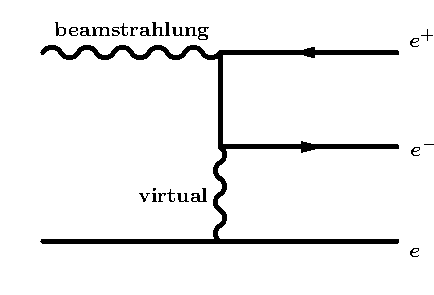
\includegraphics[width=\textwidth]{Figures/Bethe-Heitler.pdf}
\caption{Bethe-Heitler}
\end{subfigure}
\begin{subfigure}[b]{0.33\textwidth}
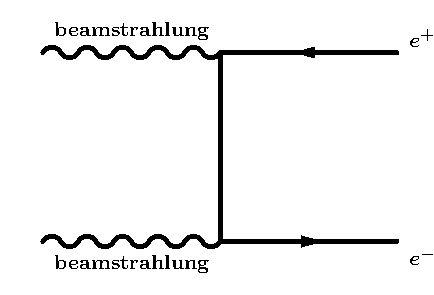
\includegraphics[width=\textwidth]{Figures/Breit-Wheeler.pdf}
\caption{Breit-Wheeler}
\end{subfigure}
\begin{subfigure}[b]{0.33\textwidth}
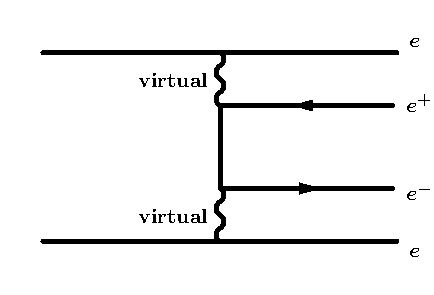
\includegraphics[width=\textwidth]{Figures/Landau-Lifshitz.pdf}
\caption{Landau-Lifschitz}
\end{subfigure}
\caption[LO Feynman diagrams of the production of the background pairs.]{The LO Feynman diagrams of the production processes of the background pairs: Bethe-Heitler, Breit-Wheeler and Landau-Lifschitz.}
\label{fig:Feynman:pair_production}
\end{figure}

\subsubsection{Bhabha scattering and $\gamma\gamma\rightarrow$hadrons}
\label{BeamBeam:bhabha_gammagamma}

\begin{figure}
\centering
\begin{subfigure}[b]{0.35\textwidth}
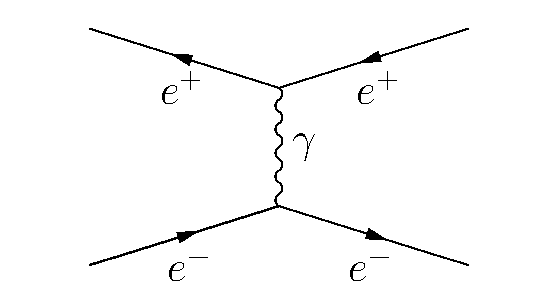
\includegraphics[width=\textwidth]{Figures/bhabha_scattering.pdf}
\caption{Bhabha scattering}
\end{subfigure}
\vspace*{0.2cm}
\begin{subfigure}[b]{0.35\textwidth}
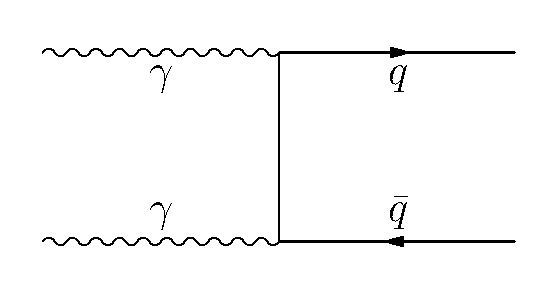
\includegraphics[width=\textwidth]{Figures/gammagamma_hadrons.pdf}
\caption{$\gamma\gamma\rightarrow$hadrons}
\end{subfigure}
\caption[LO Feynman diagrams of bhabha scattering and the $\gamma\gamma\rightarrow$hadrons process.]{The LO Feynman diagrams of the bhabha scattering and the $\gamma\gamma\rightarrow$hadrons process.}
\label{fig:Feynman:bhabha_gammagamma}
\end{figure}

\subsection{Machine backgrounds}
\label{MachineBackgrounds}
\chapter{Accelerator Physics of Linear Colliders}
\label{LinearColliderPhysics}

\begin{chapterabstract}
Since the invention of the first particle accelerator in 1930, many new forms of accelerators were discovered and developed over the years. 
Even though they may differ in shape and form, they all rely on the same principles. 
After a brief introduction of these principles of accelerator physics, there will be a description of the two classes of particle accelerators which are mainly used for high-energy physics nowadays: linear and circular colliders. 
By looking at their advantages and disadvantages, the differences between them will be elaborated.
\end{chapterabstract}
\newline

In 1930, J. D. Cockcroft and E. T. S. Walton constructed the first particle accelerator, in order to probe the nuclei of lithium atoms with protons accelerated to several hundred keV. 
They found that the key in particle acceleration lies in electrostatics.

\section{Principles of particle acceleration}
\label{AcceleratorPhysics}
Charged particles are accelerated inside an electric field. 
In a time independent electric field $\vec{E}$ with potential $U$, the particle with charge $q$ experiences a change in its kinetic energy by passing through this electric field.
\begin{equation}
 \Delta E = q \int \vec{E}d\vec{r} = qU
\end{equation}
The particle's charge expressed in the elementary charge e is simply multiplied by the electric potential in Volts to calculate the gain or loss of the particle's kinetic energy. 
Out of convenience, the unit for energy in particle physics is therefore eV.\\
By this logic a particle is accelerated to higher energies by applying higher and higher electrostatic fields. 
Exactly this was done in the beginning of particle accelerators by increasing the voltage applied to a capacitor and shooting the charged particle through. 
Unfortunately, there are limits to the amount of voltage that can be applied before an electric breakdown.
The solution seems simple: putting several capacitors in a row.
But again, this can not be done with electrostatic capacitors since the field gradient between two different capacitors is directed in the opposite direction.
A particle traveling from one capacitor to the next would then lose kinetic energy again.
A solution is quickly found by using time dependent electric fields.\\
In very simple terms, the key principles of a linear collider are thereby already explained.
Better accelerating structures such as drift chambers and later on superconducting radio frequency (RF) cavities were developed over the years.
The first linear accelerator using normal conducting drift chambers of increasing lengths was built by Rolf Wider\o e at the university of Karlsruhe in Germany.
RF fields are applied to the drift chambers such that the particles are accelerated in between the chambers when passing through the gaps.
Since the particle gains energy by passing through a gap, the chambers need to have increasing length in order to guarantee the particle being accelerated by the same phase of the RF field.
\todo{picture of linac with increasing drift chambers}
Nowadays, particle accelerators all over the world mainly use RF cavities instead of drift tubes, with the possibility of being made of superconducting material since the electric resistance is minimal due to their superconducting nature.
Unlike before the acceleration takes place inside the cavities, and all cavities are of the same length and shape.
To still guarantee the particle to be accelerated by the same RF phase, the RF frequency is varied.
\todo{picture of RF cavities}

Rolf Wider\o e did not only build the first linear accelerator, he even more importantly invented the principles of the betatron, the very first accelerating structure using electromagnetic fields.
Also the cyclotron which was invented in 1928 uses a magnetic field to deflect the charged particles on a radial path, and therefore allow the accelerating structure to be much smaller than a linear accelerator.
Exactly that idea was needed to advance particle acceleration from linear to circular.

\section{Linear colliders in comparison to circular colliders}
\label{Linear-Circular}

Circular acceleration does also have certain challenges.
Since the particle gains energy over time, the radius of its circular path increases if the magnetic field is constant.
The accelerator has to be built accordingly taking the increase in the radius into account, or needs to use magnets with variable field strengths.
Ladder is done in synchrotron machines, a type of circular accelerator combining the principles of all particle accelerators mentioned above: acceleration in RF cavities, variation of the RF frequency, and variable magnetic field strengths.
In this way, the particles are traveling along a stationary orbit, passing through the same magnets and cavities over and over again.
To insure the stability of the orbit, not only bending dipole magnets can be found but also sextupole and octupole magnets which focus the particles and correct orbit fluctuations.
Because of being accelerated by an alternating RF field, the synchrotron beams naturally form beam bunches in the following way:
With the particle momentum having a Gaussian distribution, slow particles, i.e. particles with smaller than the ideal momentum, arrive at the accelerating cavity later than the ideal particle, and faster particles earlier respectively.
Therefore particles will be accelerated by different phases of the RF field: particles arriving later will experience a higher phase and will be accelerated more, particles arriving too early will experience a smaller phase and therefore will be accelerated less.
The particles oscillate about the ideal stable phase, and therefore form beam bunches.
\todo{picture of the RF phases: Beschleunigerphysik slides}%BeschleunigerSS12_04, p.5

Currently, the world's largest circular particle collider is the Large Hadron Collider (LHC) at CERN in Switzerland, a synchrotron machine with a circumference of \SI{27}{\kilo\meter}.
The collision energy of the two colliding proton beams is \SI{13}{\TeV}, and its nominal peak luminosity \lumi is \SI{e34}{\centi\meter^{-2}\second^{-1}}.
The luminosity of a particle collider is proportional to the amount of collisions that can occur, and it is defined as:
\begin{align}
 \mathcal{L}&=\frac{N_1N_2 \cdot n_b \cdot f}{2\pi \cdot \sqrt{\sigma^2_{x,1}+\sigma^2_{x,2}} \sqrt{\sigma^2_{y,1}+\sigma^2_{y,2}}}\\
 \intertext{If the bunch sizes of the opposite beams are the same:}
 &=\frac{N_1N_2 \cdot n_b \cdot f}{4\pi \cdot \sigma_x \sigma_y}
\end{align}
$N_{1,2}$ is the number of particles per bunch, which is usually the same for both beams, so that $N_1=N_2$.
$f$ is the revolution frequency, the number of revolutions a bunch makes per second.
$n_{b}$ is the number of bunches, and $\sigma_{x,y}$ is the beam bunch size in the horizontal and the vertical plane.
Table~\ref{tab:ILC_parameters} in Chapter~\ref{ILC} lists these parameters and their values for the LHC in comparison to the International Linear Collider (ILC).
In order to translate the luminosity in an event rate, the luminosity value has to be divided by the cross-section $\sigma_p$ of the physics process that is of interest.
Since the LHC detectors do only measure events from inelastic scattering, the LHC event rate can be calculated by taking only the cross-section for inelastic proton-proton scattering into account, which is measured to be \SI{78}{\milli\barn}~\cite{inelXSection}.
\begin{align}
 \dot{N}&=\mathcal{L}\cdot\sigma_{inelastic}\\
 &=10^{34} \textrm{cm}^{-2}s^{-1} \cdot 78\textrm{\,mb}\\
 &=7.8\times 10^8 s^{-1}
\end{align}
%https://www.lhc-closer.es/taking_a_closer_look_at_lhc/0.cross_section
Per second about 780 million events are occurring at the LHC.
%The reason why large synchrotron rings need pre-accelerators is that the range for changing the magnet's field strength is limited.
The LHC is a so-called ``discovery machine''.
With its high luminosity and high collision energy, the possible physics processes from the hadron collisions cover wide energy ranges.  
New particles, first seen for example as resonance peaks in the measured mass spectra, can be discovered easier due to the large phase-space.
This was the case in 2012 for instance, when the LHC found a peak at an energy of \SI{126}{\GeV}, shortly after recognized as the very first measurement of a Higgs boson.~\cite{Higgs}

Why these so-called ``discovery machines'' are hadron and not lepton colliders, and why they are circular and not linear, is to be explained with the physical qualities of the colliding particles.
Hadrons are by definition composite particles, providing the possibility of covering a large energy range when during collision their partons are interacting.
This so-called deep inelastic scattering is explained in more detail in Chapter~\ref{StandardModel}.
In contrast to that, collision of leptons as elementary particles is the interaction of exactly these leptons at exactly their given energy.
This is one of the reasons why lepton colliders are called ``precision machines''.
\chapter{The International Linear Collider}
\label{ILC}
\begin{chapterabstract}
For answering the fundamental questions of mankind, it is necessary to understand the world in great detail.
In order to confirm theories in particle physics, or to disproof them, it is often important to be able to measure the qualities of particles or their interactions to the tenth decimal place or better.
For measurements being done in high-energy particle colliders, such precisions can only be reached in linear lepton colliders, as has already been shown in Chapter~\ref{LinearColliderPhysics}.
The following sections will present a new design for such a collider of the precision frontier: the International Linear Collider (ILC). 
Its proposed layout, the possible construction sites, the detectors, and finally the physics motivation for such a capable accelerator will be explained.
\end{chapterabstract}
\newline

The International Linear Collider (ILC) is a proposed linear \positron\electron collider with state of the art technologies for the detectors and the machine, so that high precision measurements will be possible.

\section{Motivating the layout}
\label{ILC:layout}
The ILC was originally designed to collide electron and positron beams with a center-of-mass energy of \SI{500}{\GeV} in the first stage of operation.
Because of political developments and the request in 2017 to reduce the construction cost, the first stage collision energy was reduced to \SI{250}{\GeV}.
Due to the fact that linear colliders can be extended in length, the beam energies can linearly be increased.
Therefore, the ILC has the possibility to upgrade the machine to higher energies later on.

\subsection{The Layout}
Figure~\ref{fig:ILC_Layout} shows the schematic layout of the ILC.
\begin{figure}
\centering
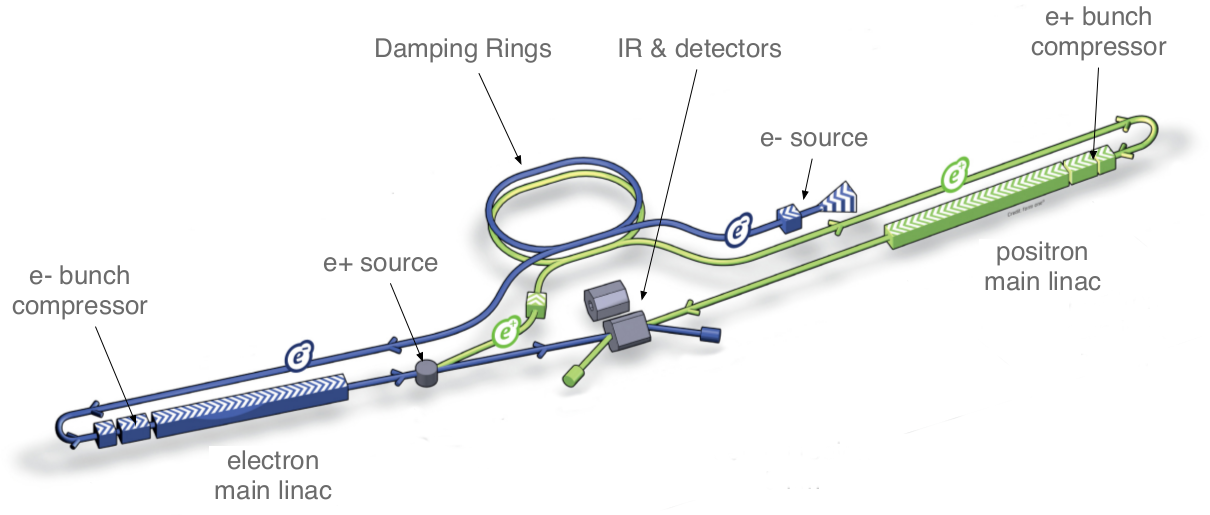
\includegraphics[width=\textwidth]{Figures/ILC_layout_edited.png}
\caption[Schematic layout of the ILC]{Schematic layout of the ILC~\cite[cf. p. 9]{TDR1}}
\label{fig:ILC_Layout}
\end{figure}\todo{I have edited this figure slightly -> how to do the citation correctly?}
The electrons are produced by a photo-cathode.
By shining a circularly polarized laser on the electron beam, one reaches a beam polarization of at least 80\,\%, i.e. more than 80\,\% of all electrons will be left-handed\footnote{For a left-handed particle, its spin and its momentum are antiparallel, pointing in opposite directions.}:
\begin{equation}
 P_e = \frac{N_L-N_R}{N_L+N_R} > 0.8
\end{equation}
The positron source consists of an undulator and a conversion target.
In an undulator, several dipole magnets are placed in a line in such a way that their polarity alternates periodically (see Figure~\ref{fig:Undulator}).
For the creation of the positrons, the actual electron beam is used, which is guided through the undulator.
By doing so, the electrons are deflected several times and emit synchrotron radiation photons, as explained in Chapter~\ref{AccPhysics:Linear-Circular}.
The photons are then converted in the conversion target, where \positron \electron pairs are produced due to pair production.
The positrons are captured and form the positron beam.\todo{Which material is the conversion target in the positron source? What is the positron production efficiency?}
\begin{figure}
\centering
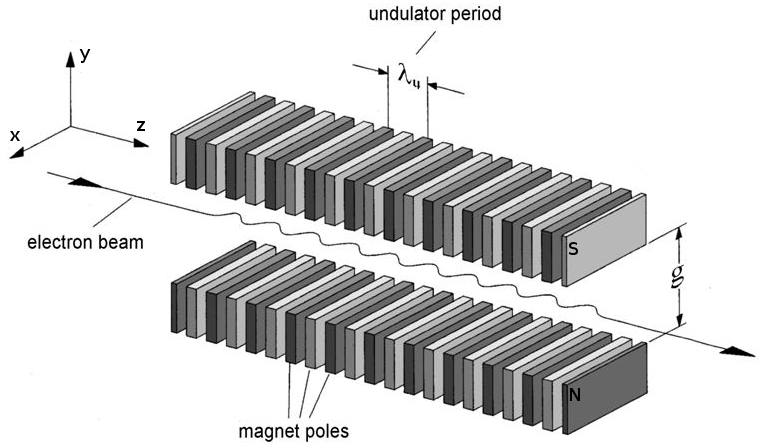
\includegraphics[width=0.8\textwidth]{Figures/Undulator_edited.png}
\caption[Schematic layout of an undulator]{Schematic of an electron beam traveling through an undulator with dipole magnets in alternating order.~\cite[cf. p. 41]{Wille}}
\label{fig:Undulator}
\end{figure}\todo{I have edited this figure slightly -> how to do the citation correctly?}
The polarized positrons continue in the positron line which is from that point on equivalent to the electron line.\todo{positron polarization?}
Since the electrons and positrons have a large emittance when they originate from their sources, their momentum and beam size have to be condensed.
This is done in the damping rings (DR), which have a circumference of \SI{3.2}{\kilo\meter}.
As discussed several times before, the beams will emit synchrotron radiation when they are deflected in the magnetic field of dipole magnets.
Exactly this is desired in the damping rings in order to ``cool'' the beams, i.e. to reduce their momentum due to the emission of light.
In a second step the beams are then accelerated again which increases their momentum in the desired direction.
The result is a high quality beam with small beam emittance.\\
After passing the damping rings, the electron and positron beams are compressed into bunches by a two-stage compressor system.
Subsequent to that, the bunches are injected into the main linear accelerator structures (linacs).
The main linacs have a length of \SI{5}{\kilo\meter}, and use superconducting RF cavities which are shown in Figure~\ref{fig:Tesla_Cavity}. 
For the machine upgrade to \SI{500}{\GeV}, the linacs can be extended in length.
Since these exact cavities are already in use for the European XFEL (X-Ray Free-Electron Laser) at Deutsches Elektronen-Synchrotron (DESY) in Hamburg, their high performance has been demonstrated.
It has been shown that they have an average accelerating gradient of \SI{31.5}{MV/m}, and that they can be operated with a frequency of \SI{1.3}{\giga\hertz}.\\
The Beam Delivery System (BDS), which has an overall length of about \SI{4.4}{\kilo\meter}, transports the bunches from the linacs to the Interaction Point (IP).
In the BDS, the beams are focused to nanometer size by the Final-Focus (FF) system.
The Final-Focus system is a crucial part of the ILC program.
Only with nanometer-sized beams, the ILC can reach luminosities comparable to or beyond the LHC.
To demonstrate the feasibility of nanometer-scale beams, a test facility was build that is a small scale prototype of the FF system for the ILC: the Accelerator Test Facility (ATF2), which will be presented in more detail in Section~\ref{ATF2}.
\\After the Final-Focus system, the beams are then finally brought into collision with a crossing angle of \SI{14}{mrad} at the IP.\cite[p. 9-10]{TDR1}
Table~\ref{tab:ILC_parameters} shows the machine parameters for the baseline design at \SI{250}{\GeV} center-of-mass energy, and for the luminosity and the energy upgrade stages.


%\multicolumn{1}{>{\centering}p{1.5cm}}{\textbf{Baseline 500}} & \multicolumn{1}{>{\centering}p{1.5cm}}{\textbf{Lumi Upgrade}} & \multicolumn{1}{>{\centering}p{1.5cm}}{\textbf{TeV Upgrade}} & {\centering\textbf{LHC 25ns}} \\ 

\begin{table}
\caption{Beam parameters for different phases in the ILC operation scenario (ILC250, Baseline 500, Luminosity Upgrade, TeV Upgrade)~\cites[p. 11]{TDR1}{CR-0016} in comparison to LHC beam parameters~\cite{SiDBkgNote}}.
\label{tab:ILC_parameters}
\centering
\begin{tabularx}{0.92\textwidth}{ll|rrrrg}
\hline\hline
& & \multicolumn{1}{>{\centering}p{2cm}}{\textbf{ILC250}} & \multicolumn{1}{>{\centering}p{2cm}}{\textbf{Baseline 500}} & \multicolumn{1}{>{\centering}p{2cm}}{\textbf{Lumi Upgrade}} & \multicolumn{1}{>{\centering}p{2cm}}{\textbf{TeV Upgrade}} & \textbf{LHC 25ns}\\
\hline
\cline{1-7}
\hline
E$_{CM}$  &(\si{\GeV})& 250 & 500  & 500  & \num{1000} & \num{14000}\\
n$_b$ & & \num{1312} & \num{1312} & \num{2625} & \num{2450} & \num{2808} \\
$\Delta t_b$ &(\si{\nano\second}) & 554 & 554  & 366   & 366 & 25\\
N & & \num{2.0e10} & \num{2.0e10}  & \num{2.0e10}  & \num{1.74e10} & \num{11.5e10} \\
q$_b$ &(\si{\nano\coulomb})  & 3.2 & 3.2  & 3.2  &  2.7 & 18.4  \\
$\sigma_x^*$ &(\si{\nano\metre}) & 515.5 & 474  & 474  &  481 & \num{16700}\\
$\sigma_y^*$ &(\si{\nano\metre}) & 7.7 & 5.9 &  5.9  &  2.8 & \num{16700}\\
$\sigma_z$ &(\si{\milli\metre}) & 0.3 & 0.3  &  0.3  &  0.25 & 0.755\\
L &(\si{\per\centi\metre\squared\per\second}) & \num{1.35e34} & \num{1.8e34} & \num{3.6e34} & \num{3.6e34} & \num{1.0e34}\\
\hline\hline
\end{tabularx}
\end{table}

The Interaction Region (IR) houses the two detectors for the ILC, the Silicon Detector (SiD) and the International Large Detector (ILD), which are in a push-pull system.
The detectors and the push-pull system are explained in more detail in Section~\ref{ILC:detectors}.

\subsection{Physics Motivation}
\label{ILC:physicsmotivation}

The ILC can be motivated in different ways.
First, the advantages it will have over hadron colliders can be summarized with only four key words.
Second, the ILC will be a Higgs factory which will measure the qualities of the Higgs boson with much higher precision than it had been done so far.
Additionally, the ILC will not only be a Higgs factory but will also measure the Top quark qualities, and will have access to Beyond Standard Model (BSM) physics.\\
The following paragraphs will go into more detail about the first two points and will motivate on the basis of these points why the ILC is a great machine.

\subsubsection{Key words}
The physics motivation for the ILC can be summarized with four key words: Cleanliness, Democracy, Calculability and Detail.\cite[p. 2-5]{TDR2}
In the following, the meaning of these key words will be explained with respect to the great advantages the ILC has in comparison to hadron colliders, like the LHC.
\paragraph{Cleanliness}
Cleanliness describes the clean events the detectors at the ILC will record.
The environment is clean because of the small background levels and therefore small detector occupancy in comparison to a hadron collider.
Due to the polarization of both beams, there are only events with couplings to electroweak interactions, which reduces the background level.
The energy range is restricted, since the initial energy of the colliding beams can be set precisely and only point-like particles collide.
Therefore, there are no underlying events which arise from the other nuclei of the composite particle, like in a proton-proton collider.

\begin{figure}
\centering
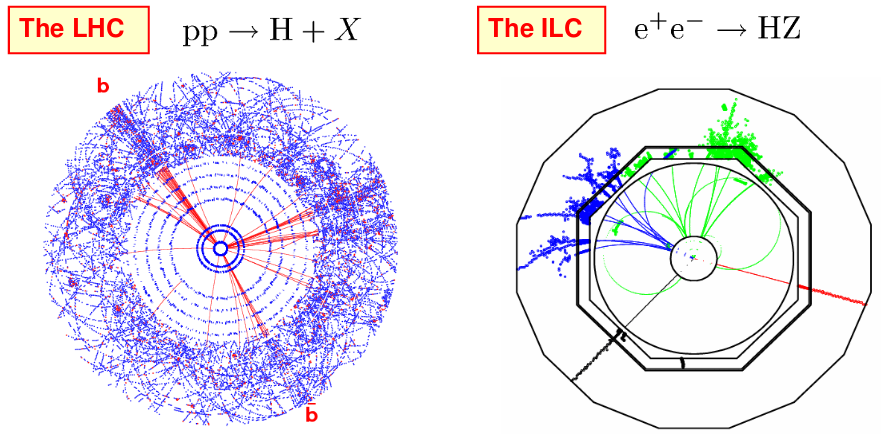
\includegraphics[width=0.5\textwidth]{Figures/Cleanliness.png}
\caption[Clean environment at the ILC]{Comparison of the event displays of a Higgs event at the  LHC and at the ILC.\cite[p. 4]{ILCPhysics_Thomson}\\
The comparison shows that at the ILC the hits recorded are exclusively from the final state particles of the physics interaction.
At the LHC, underlying and pileup events populate the detector.}
\label{fig:Cleanliness}
\end{figure}

\paragraph{Democracy}
Because the elementary coupling e of photons is the same for all quarks and leptons, the \electron \positron annihilation produces pairs of all species, from the Standard Model and Beyond Standard Model, at similar rates.
Besides that, the ILC will be taking data without triggers, i.e. all events will be recorded.
This is possible because of the Cleanliness.
\paragraph{Calculability}
The energies involved in the initial states are precisely known, since there are only point-like elementary particles in initial state.
There are only events with couplings to electroweak interactions.
Additionally, systematic uncertainties due to PDF uncertainties and QCD corrections are omitted.
\paragraph{Detail}
Because of the clean events and the possibility to record and store all taken data, events can be reconstructed in completeness without theoretical assumptions.
The quark and lepton momenta can therefore be determined by kinematic fits.
Studies of the spin-dependence of the production and decay processes are also possible.\\
Due to the high energy resolution and the fact that the initial particle energies are precisely known, particles with small mass differences are distinguishable, i.e. peaks in mass spectra that are close together are more likely to be separable.\\
Additionally, the nano-sized beam of the ILC allows the vertex detector to be close to the IP. 
Hence, c-tagging is possible at the ILC which improves a lot of physics studies.

\subsubsection{ILC as a Higgs factory}
One could call the ILC a Higgs factory, since the total cross section for Higgs production is 10\textsuperscript{-2} in comparison to 10\textsuperscript{-9} for the LHC for example.
%TODO : Find source or plot that shows the total production cross sections at ILC and LHC
Therefore, the number of Higgs events measured at the ILC will be significantly higher, namely about 10 Higgs events per hour.
Due to the large statistics and the capability for precision measurements, the individual Higgs couplings can be measured to a percent accuracy and the global width of the Higgs can be measured directly.
When taking the LHC as an example, the LHC experiments have to make a global fit to all Higgs signals and make assumptions of the Higgs width, in order to get the Higgs couplings.
This can not be as precise as at the ILC, as can be seen in Figure~\ref{fig:Higgs_couplings}.
Only for the coupling to photons, the LHC yields more precise measurements which can only be topped by the combination of the LHC and the ILC results.

\begin{figure}
\centering
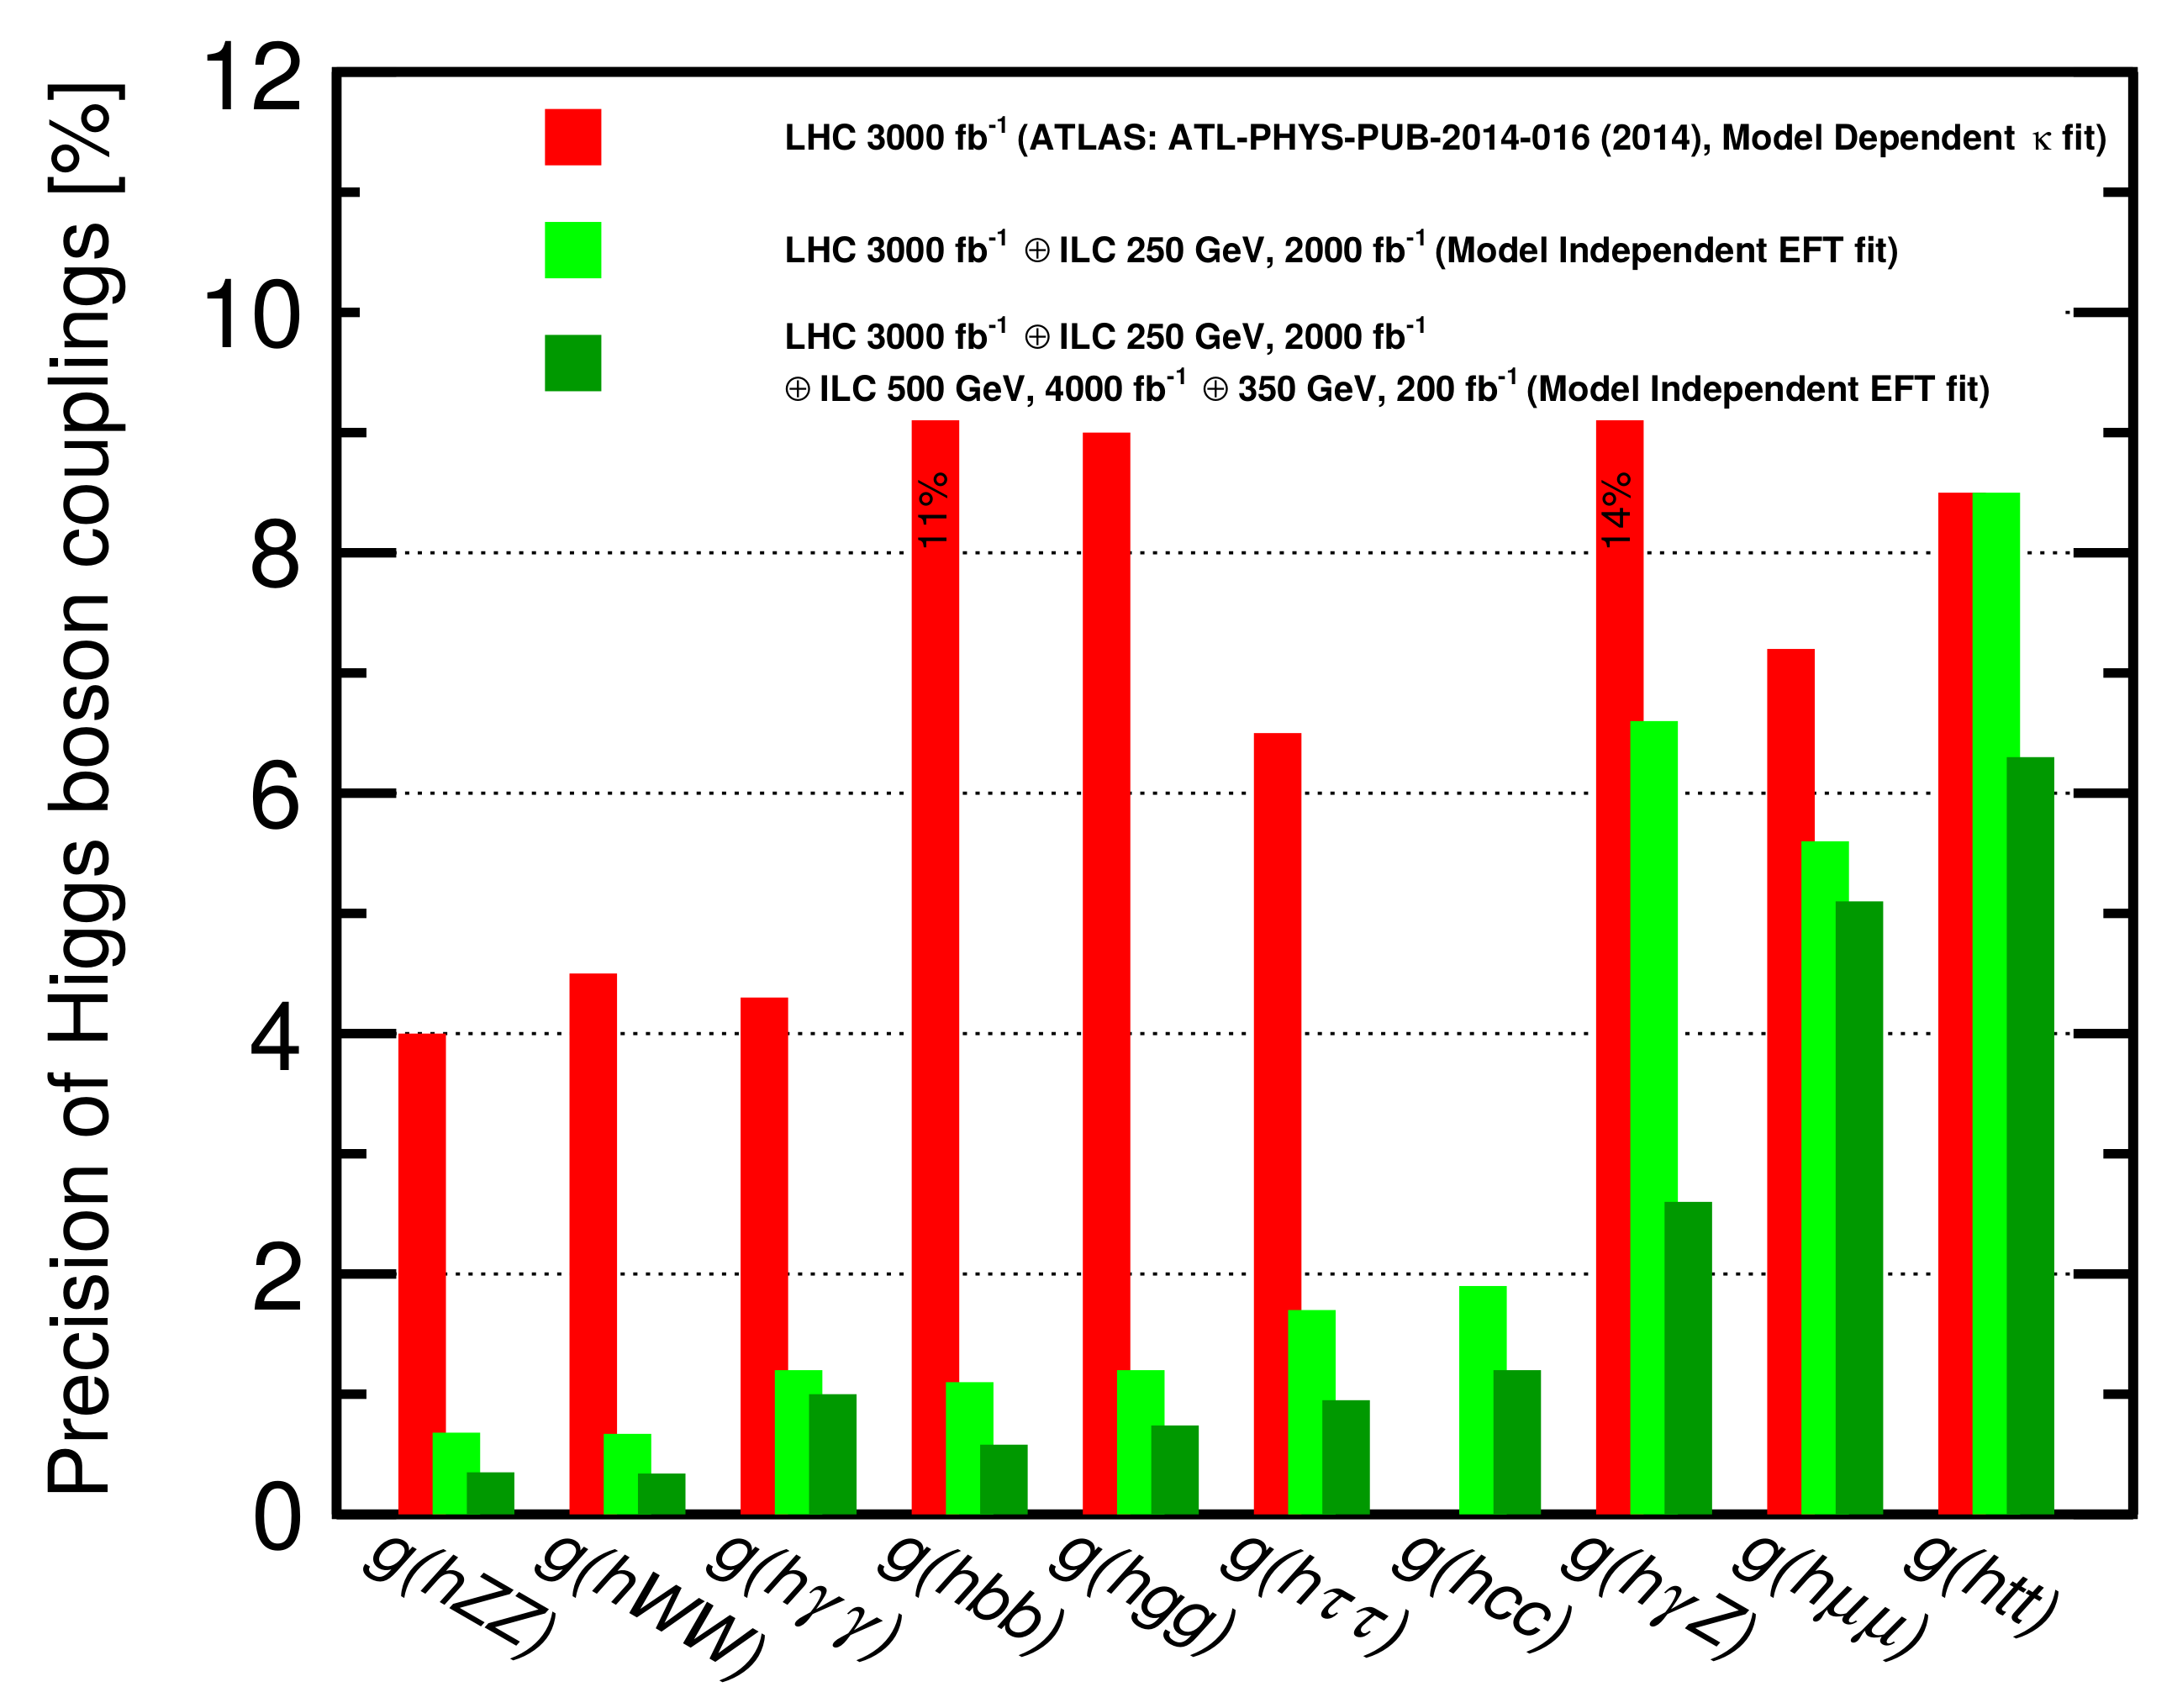
\includegraphics[width=0.5\textwidth]{Figures/Higgs_couplings.png}
\caption[Higgs coupling precisions]{Comparison of the Higgs coupling precision reached at the ILC and at the LHC.\cite[p. 9]{ILCPhysics}\\
The plot shows the relative precisions for the Higgs couplings calculated from the model-dependent fits to simulated data from the High-Luminosity LHC and the ILC.}
\label{fig:Higgs_couplings}
\end{figure}
%TODO : Check if there is a more up-to-date picture

\section{Possible Site}
\label{ILC:site}
Out of originally 10 potential ILC sites in Japan, the Kitakami mountains in the Tohuku Prefecture was chosen to be the preferred site for the ILC.
This decision was made in July 2013 after a detailed study of all site specific factors, like the geological conditions, the infrastructure, and the impact on the environment and the economy.
As can be seen in Figure~\ref{fig:ILC_Site}, the closest city with about 120,000 citizens would be Ichinoseki.
Morioka and Sendai are the biggest cities around the candidate site, with Tokyo being about \SI{430}{\kilo\meter} away.
Although being in the north of Japan, the travel time from Tokyo is only about three hours, and the proximity to the coast line allows the transportation of construction, machine and detector parts by ship.

\begin{figure}
\centering
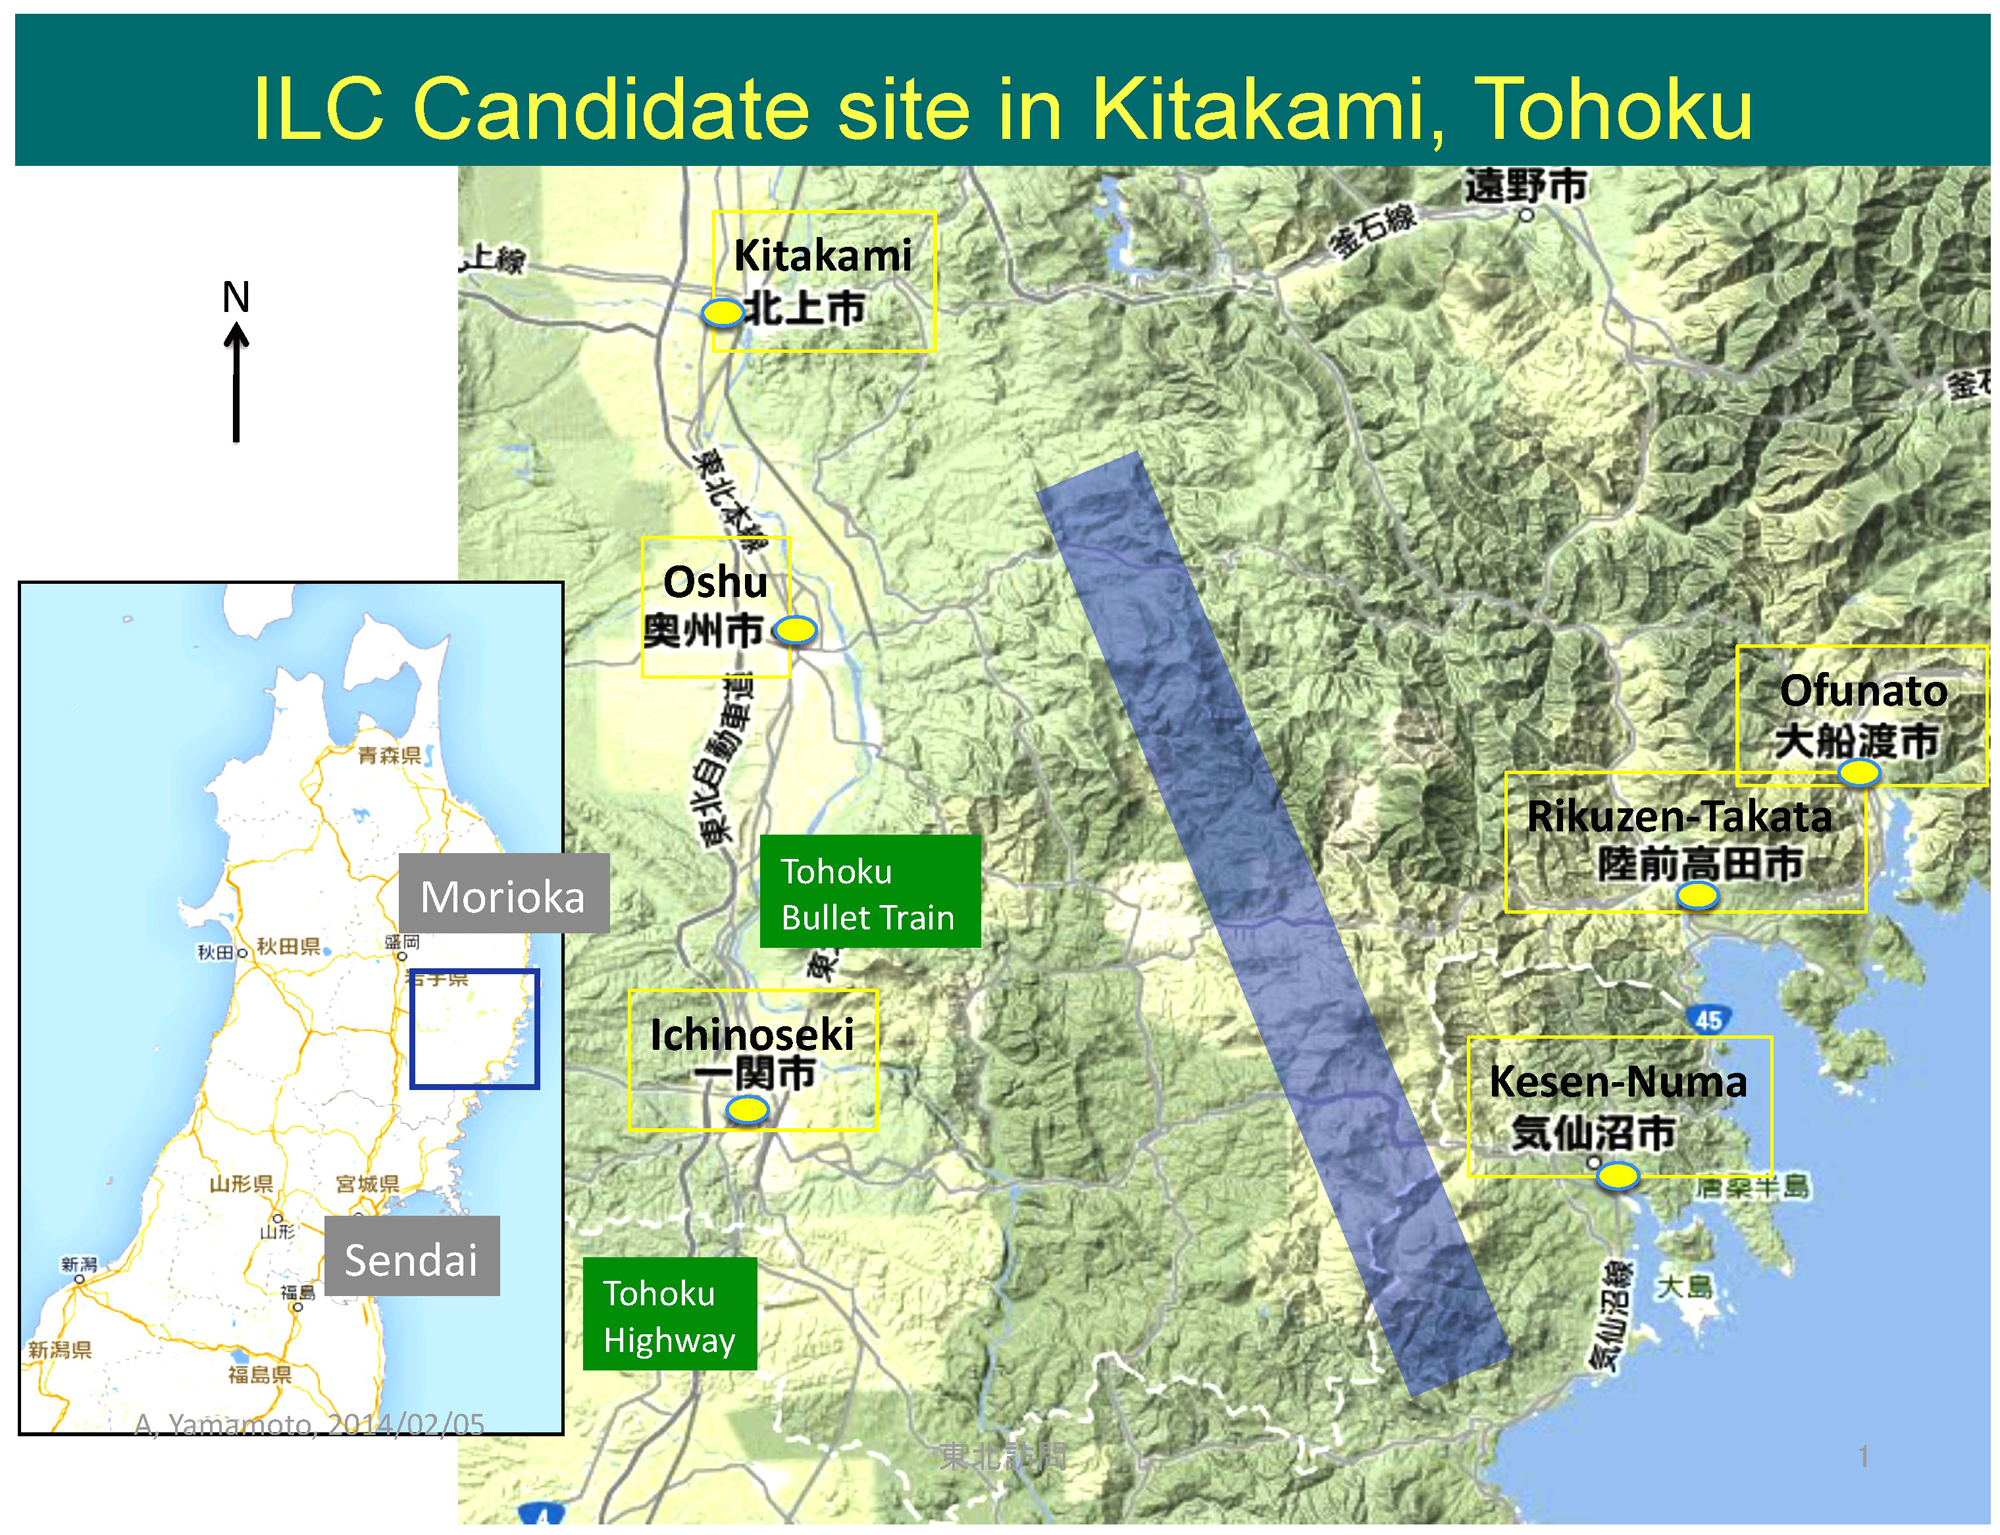
\includegraphics[width=0.6\textwidth]{Figures/ILC-site.jpg}
\caption[Possible site for the ILC]{The possible site for the ILC are the Kitakami mountains in the Tohuku Prefecture.\cite{Site}}
\label{fig:ILC_Site}
\end{figure}

\section{The Experiments}
\label{ILC:detectors}

In order to preserve the competitive spirit and the ability to cross-check results, the ILC has two detectors despite the fact that it is a linear and not a circular collider.
The so-called push-pull system makes that possible by allowing the detectors to switch position after a certain amount of data-taking time.
The whole detector together with the last quadrupole magnet of the accelerator Final Focus system will be pulled out of the beam line, and the other one will be pushed in.
The whole process is designed to take only a short time, i.e. several hours up to 1-2 days, but involves some challenges especially for the magnets, the cryogenics and the detector and machine alignment.\cite[p. 28-29]{TDR1}
The two detectors, the Silicon Detector (SiD) and the International Large Detector (ILD), will be explained in detail in the following with a bigger focus on the SiD detector since some of the background studies presented in the thesis were made for the SiD only.

\subsection{The Silicon Detector}
The SiD is designed to be a robust, compact detector with the vertex and tracker subdetectors and the electromagnetic calorimeter (ECAL) being based on silicon sensors.
The silicon design in comparison to other designs for the vertex and tracking detectors is more robust regarding the beam background and timing.
With also the highly segmented hadronic calorimeter being inside the solenoid field, particle tracking is possible even in the calorimeters.
With being designed to be compact, the measurements for the full detector are \SI{14}{m} in height and \SI{11}{m} in length.
To compensate the small radius, so that SiD is still hermetic and contains the full particle showers, the magnetic field of the superconducting solenoid magnet is \SI{5}{T}.

Figure~\ref{fig:SiD} shows schematic drawings of the SiD detector and its subdetectors.

\begin{figure}
\centering
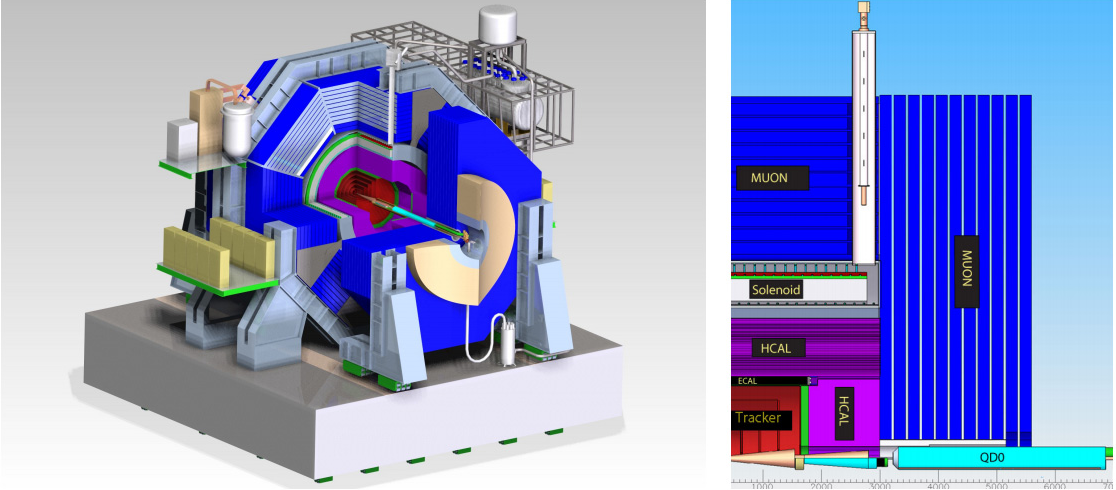
\includegraphics[width=0.7\textwidth]{Figures/SiD.png}
\caption[Schematic drawing of the SiD detector]{The SiD detector consists of the vertex and tracking detectors (red), the electromagnetic calorimeter (ECAL) (green), the hadronic calorimeter (HCAL) (purple) and the muon system (blue). All subdetectors except the muon system are inside the solenoid magnet.\cite[p. 31]{TDR1}}
\label{fig:SiD}
\end{figure}
%TODO : Update the picture of the SiD detector -> new design for muon system

Overall the SiD detector is optimized for Particle Flow Algorithms (PFA).
PFA is a reconstruction method that reconstructs each particle of the final state individually and uses the different subdetectors for a specific purpose.
Therefore, charged particles are reconstructed from tracks in the tracker device, the ECAL is used for photons, and the ECAL and HCAL together for other neutral particles. 
%TODO : Find a source for explanation of PFA

Table~\ref{tab:KeyParametersSiD} lists the key parameters and measurements of the SiD subdetector systems.

\begin{table}
\caption{Key parameters of the baseline SiD design. All dimensions are given in cm.\cite{SiDBkgNote}}
\label{tab:KeyParametersSiD}
\centering
\begin{tabularx}{0.81\textwidth}{l|llll}
\hline\hline
SiD Barrel & Technology & Inner radius & Outer radius & z extent\\
\hline
Vertex detector & Silicon pixels & 1.4 & 6.0 & $\pm 6.25$ \\
Tracker & Silicon strips & 21.7 & 122.1 & $\pm 152.2$ \\
ECAL & Silicon pixels-W & 126.5 & 140.9 & $\pm 176.5$ \\
HCAL & RPC-steel & 141.7 & 249.3 & $\pm 301.8$ \\
Solenoid & 5 T SC & 259.1 & 339.2 & $\pm 298.3$ \\
Flux return & Scintillator-steel & 340.2 & 604.2 & $\pm 303.3$ \\
\hline
SiD Endcap & Technology & Inner z & Outer z & Outer radius\\
\hline
Vertex detector & Silicon pixels & 7.3 & 83.4 & 16.6 \\
Tracker & Silicon strips & 77.0 & 164.3 & 125.5 \\
ECAL & Silicon pixel-W & 165.7 & 180.0 & 125.0 \\
HCAL & RPC-steel & 180.5 & 302.8 & 140.2 \\
Flux return & Scintillator/steel & 303.3 & 567.3 & 604.2 \\
LumiCal & Silicon-W & 155.7 & 169.55 &  20.0 \\
BeamCal & Semiconductor-W & 326.5 & 344 & 14.0 \\
\hline\hline
\end{tabularx}
\end{table}

\subsection{The International Large Detector}

Like the SiD detector, ILD is a multi-purpose particle detector that is optimized for PFA.
Its vertex detector is also based on silicon sensors, whereas the tracker is a combination of both, a silicon strip and pixel detector and a time projection chamber (TPC).
Also similar to SiD, the calorimeters are within the solenoid magnet, which is only surrounded by the muon system.
The magnetic field of the superconducting solenoid magnet is \SI{3.5}{T} for the ILD.
Because of having a big gaseous volume, the full detector is bigger than SiD, namely \SI{16}{m} in height and \SI{14}{m} in length.
Figure~\ref{fig:ILD} shows all the subdetectors mentioned above in two schematic drawings of the ILD detector.

\begin{figure}
\centering
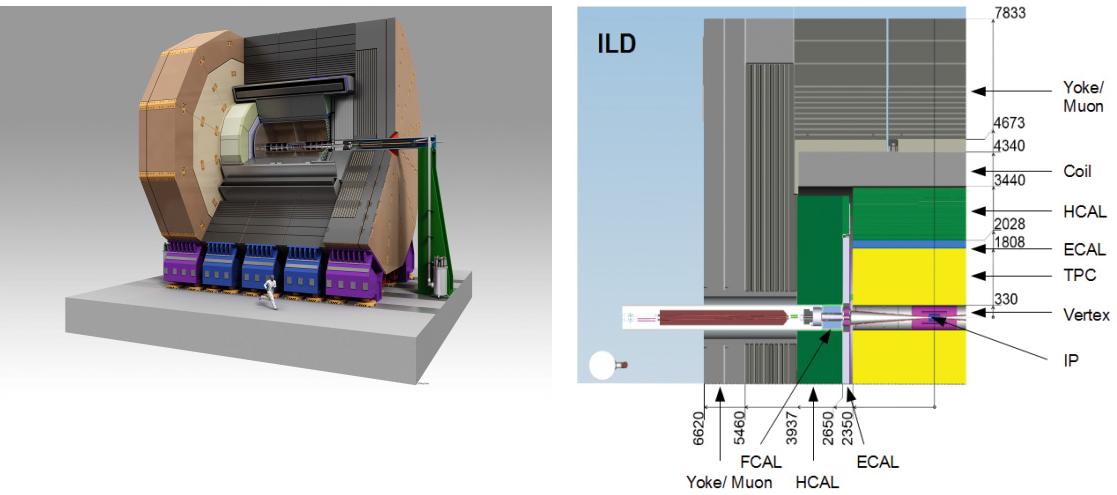
\includegraphics[width=0.7\textwidth]{Figures/ILD.png}
\caption[Schematic drawing of the ILD detector]{The ILD detector consists of the vertex detector (pink), the time projection chamber (TPC) (yellow), the electromagnetic calorimeter (ECAL) (blue), the hadronic calorimeter (HCAL) (green) and the muon system (gray). All subdetectors except the muon system are inside the solenoid magnet.\cite[p. 34]{TDR1}}
\label{fig:ILD}
\end{figure}
%TODO : Check if I have to update the picture of the ILD detector

\chapter{Background from beam-beam interactions}
\label{BeamBeam}
\section{Physics}
\label{BeamBeam:physics}
\section{Pair background}
\label{BeamBeam:pairs}
\subsection{GuineaPig}
\section{Bhabha scattering}
\label{BeamBeam:bhabha}
\subsection{Pythia}
\section{$\gamma\gamma\rightarrow$hadrons}
\label{BeamBeam:gammagamma}
\subsection{Pythia}

\chapter{BDS and Final-Focus system as background sources}

\begin{chapterabstract}
 In this chapter, two of the sources for background at the interaction point (IP) coming directly from the Beam Delivery System (BDS) and the Final-Focus System (FF) are discussed: the background from beam halo collimators, and from muon spoilers.\\For the first, simulations with \bdsim were done, and data was taken at the ATF2 test bench facility where a new beam halo collimator was installed.\\For the latter, simulations with \mucarlo are shown, and the physics behind the background generation is explained.
\end{chapterabstract}


\section{Background from Beam Halo Collimators in the Final-Focus system}

The Final-Focus System (FF) is -as explained in Chapter~\ref{ILC}- responsible for focussing the beam to nanometre size. The reason behind this is the need for high luminosities which can be gained by small beam sizes. Another goal of the International Linear Collider is to have clean events with as little background as possible. A solution to this is to install beam halo collimators in the FF system that cut off the halo around the beam core. As the beam halo can interact with the beam pipe and its components, a beam halo collimation system plays an important role in the reduction of background at the IP. Nevertheless, the collimator itself can be source to particle showers and rises in the background level around the collimator location. Feasibility studies are needed to investigate in the effect of a beam halo collimator.\\
A vertical beam halo collimator was installed at the Accelerator Test Facility 2 (ATF2) at the research centre KEK in Japan. In March 2016, data of the background was taken with a Cherenkov detector in dependency of the aperture of this collimator at ATF2. This section covers the analysis of the data as well as the comparison of the data with simulations done with \bdsim. Both, the design of the vertical beam halo collimator at ATF2 and the \geant simulation tool \bdsim are explained here additionally.

\subsection{Beam Halo Collimator}
\label{Collimator}

The vertical beam halo collimator, for which the design drawings are shown in Figure~\ref{fig:collimator}, was installed in ATF2 in the beginning of March 2016. The collimating jaws are inside a structure that is evacuated and connected to the beam pipe of the ATF2 beam line. The actual jaws are made of Copper, the rest of the components in the collimator structure are out of Stainless Steel.
%TODO: Add information about measurements of the jaws and the whole structure

\begin{figure}
\centering
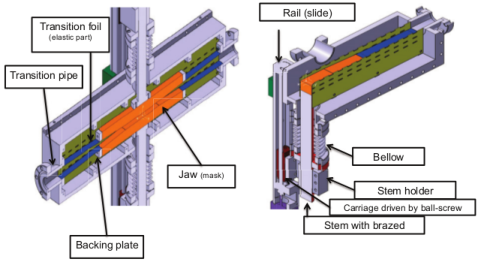
\includegraphics[width=0.8\textwidth]{ATF2_beamhalo_collimator.pdf}
\caption[Drawing of the beam halo collimator]{A drawing of the vertical beam halo collimator built into ATF2.\cite{NuriaCollimator2015}}
\label{fig:collimator}
\end{figure}

The two jaws can be moved individually to an arbitrary position, so that the edge of the jaw has a distance of between 2.6 and \SI{12}{\milli\metre} with respect to the centre. Therefore, the full aperture of the collimator structure can be between 5.2 and \SI{24}{\milli\metre}. The error on the position of the jaws is about \SI{0.04}{\milli\metre}.\\
As every component in a beam line, especially for such small beam sizes, is affecting the electromagnetic field of the passing beam, the collimator is designed to minimize the effect of inducing large wakefield. The concern of wakefields induced by the collimator is addressed in .%TODO: cite:%\bibitem{Collimator} N. Fuster-Martínez, IFIC (CSIC-UV), et al. \emph{Design study and construction of a transverse Beam Halo Collimation system for ATF2}, 2015. \url{http://accelconf.web.cern.ch/AccelConf/IPAC2015/papers/wepmn059.pdf}
This thesis focusses exclusively on the effect on the background level.

%TODO: Pictures of installed collimator

\subsection{The Accelerator Test Facility 2}
\label{ATF2}

The Accelerator Test Facility 2 (ATF2) is an extension to the accelerator facility ATF at the research centre KEK in Japan. As can be seen in Figure~\ref{fig:ATF}, ATF consists of a linear accelerator which pre-accelerates the particles before they are accessing the dumping ring. Before the ATF2 was built, the beams were dumped after leaving the dumping ring through the short extraction line.\\ATF2 is a test bench for the FF system of the ILC and has two main goals: Focussing the low-emittance beam to \SI{37}{\nano\metre} in the vertical plane, and demonstrating the stability of the nanometre sized beam at the interaction point. So far a repeatable beam size of \SI{40}{\nano\metre} has been shown. Although the beam size goal of ATF2 seems to be too large compared to the ILC goal of \SI{9}{\nano\metre}, the ATF2 system is very close to the ILC FF. The beam size goal has to be scaled up for different lattice and beam conditions.

\begin{figure}
\centering
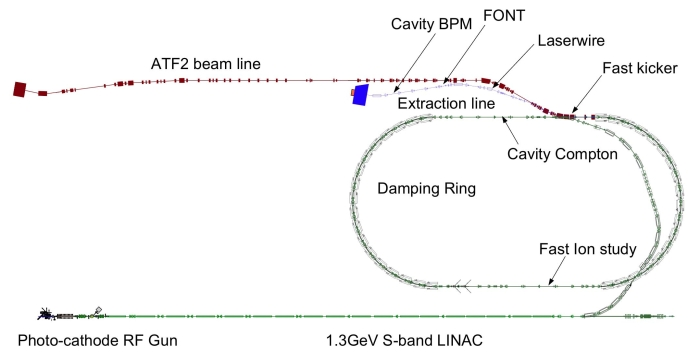
\includegraphics[width=0.6\textwidth]{ATF.jpg}
\caption[ATF accelerator]{A schematic of the ATF accelerator with the ATF2 extension. The ATF consists of a linear accelerator, a beam dump, the old extraction line, and the new ATF2 extension.}%TODO: cite the source of the ATF figure!
\label{fig:ATF}
\end{figure}

The vertical beam halo collimator and the Cherenkov detector, with which the background level in dependency of the collimator aperture was measured, are both located in the Final-Focus region of ATF2. The location of the collimator was chosen in such a way that the phase of the beta function is the same as at the IP. Due to that the effect of the collimation of the beam halo is then visible at the IP as desired. A schematic of the ATF2 lattice with the beam halo collimator and the Cherenkov detector is shown in Figure~\ref{fig:ATF2}. The Cherenkov detector was built and setup by a group of the Royal Holloway University of London (RHUL) because of which the detector is in the following referred to as the 'RHUL Cherenkov detector'. A more detailed description of this detector is given in Section~\ref{RHUL}.

\begin{figure}
\centering
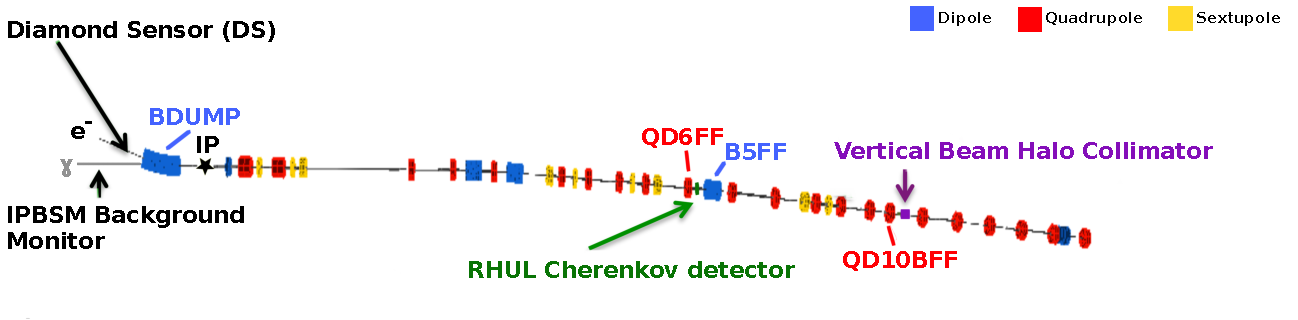
\includegraphics[width=\textwidth]{ATF2schematic.pdf}
\caption[ATF2]{A schematic of the ATF2 lattice. The beam direction is from right to left. The different magnets of the lattice are colour schemed: the bending dipole magnets are coloured in blue, the quadrupoles in red, and the sextupoles in yellow. The beam halo collimator is located before the quadrupole magnet 'QD10BFF', and the Cherenkov detector downstream between the dipole magnet 'B5FF' and the quadrupole magnet 'QD6FF'. After the interaction point (IP), the electron beam is bend in the last dipole magnet 'BDUMP' towards the beam dump. The neutral particles, like the photons, are continuing in a straight line where they can be monitored by the IPBSM Background Monitor. The Diamond Sensor (DS) can measure the shape of the beam core and the halo, before the beam is dumped.}
\label{fig:ATF2}
\end{figure}

\subsection{BDSIM}
\label{BDSIM}
\bdsim is a \geant extension toolkit for simulation of particle transport in accelerator beamlines. It was developed and is still supported by RHUL.
The geometry of lattice parts are described in classes within the \bdsim framework. Lattices, like the ATF2 lattice, can easily be built up by the pre-defined components. A figure of the ATF2 lattice visualized with the \bdsim software is shown in Figure~\ref{fig:ATF2_BDSIM}.
\begin{figure}
\centering
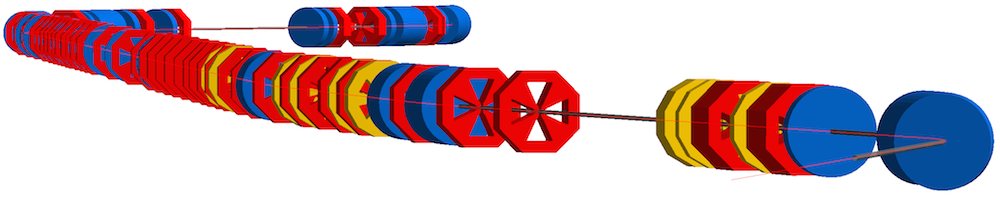
\includegraphics[width=0.7\textwidth]{atf_bdsim.png} %TODO: exchange with a recent one of ATF2
\caption[ATF2 lattice in \bdsim]{A part of the ATF2 lattice visualized with the \geant toolkit \bdsim.}
\label{fig:ATF2_BDSIM}
\end{figure}
Accelerator descriptions from other tools such as MADX can be converted to \bdsim input. 
%---------------------------------------------------
\subsection{Background studies}
\subsubsection{RHUL Cherenkov detector}
\label{RHUL}

The RHUL Cherenkov detector was built by a group from the Royal Holloway University of London. It uses the Hamamatsu PMT, which was used for a laserwire sensor that was located at the same position before. The Cherenkov detector itself is using aerogel\footnote{SP15, index 1.015, 4 slices, 4 cm$^2$, 5 cm deep}. A light pipe, with a profile area of \SI{10}{\centi\metre\square} and a total length of \SI{35}{\centi\metre}, directs the light from the aerogel to the PMT.\\
Pictures: setup\\
\begin{figure}
\centering
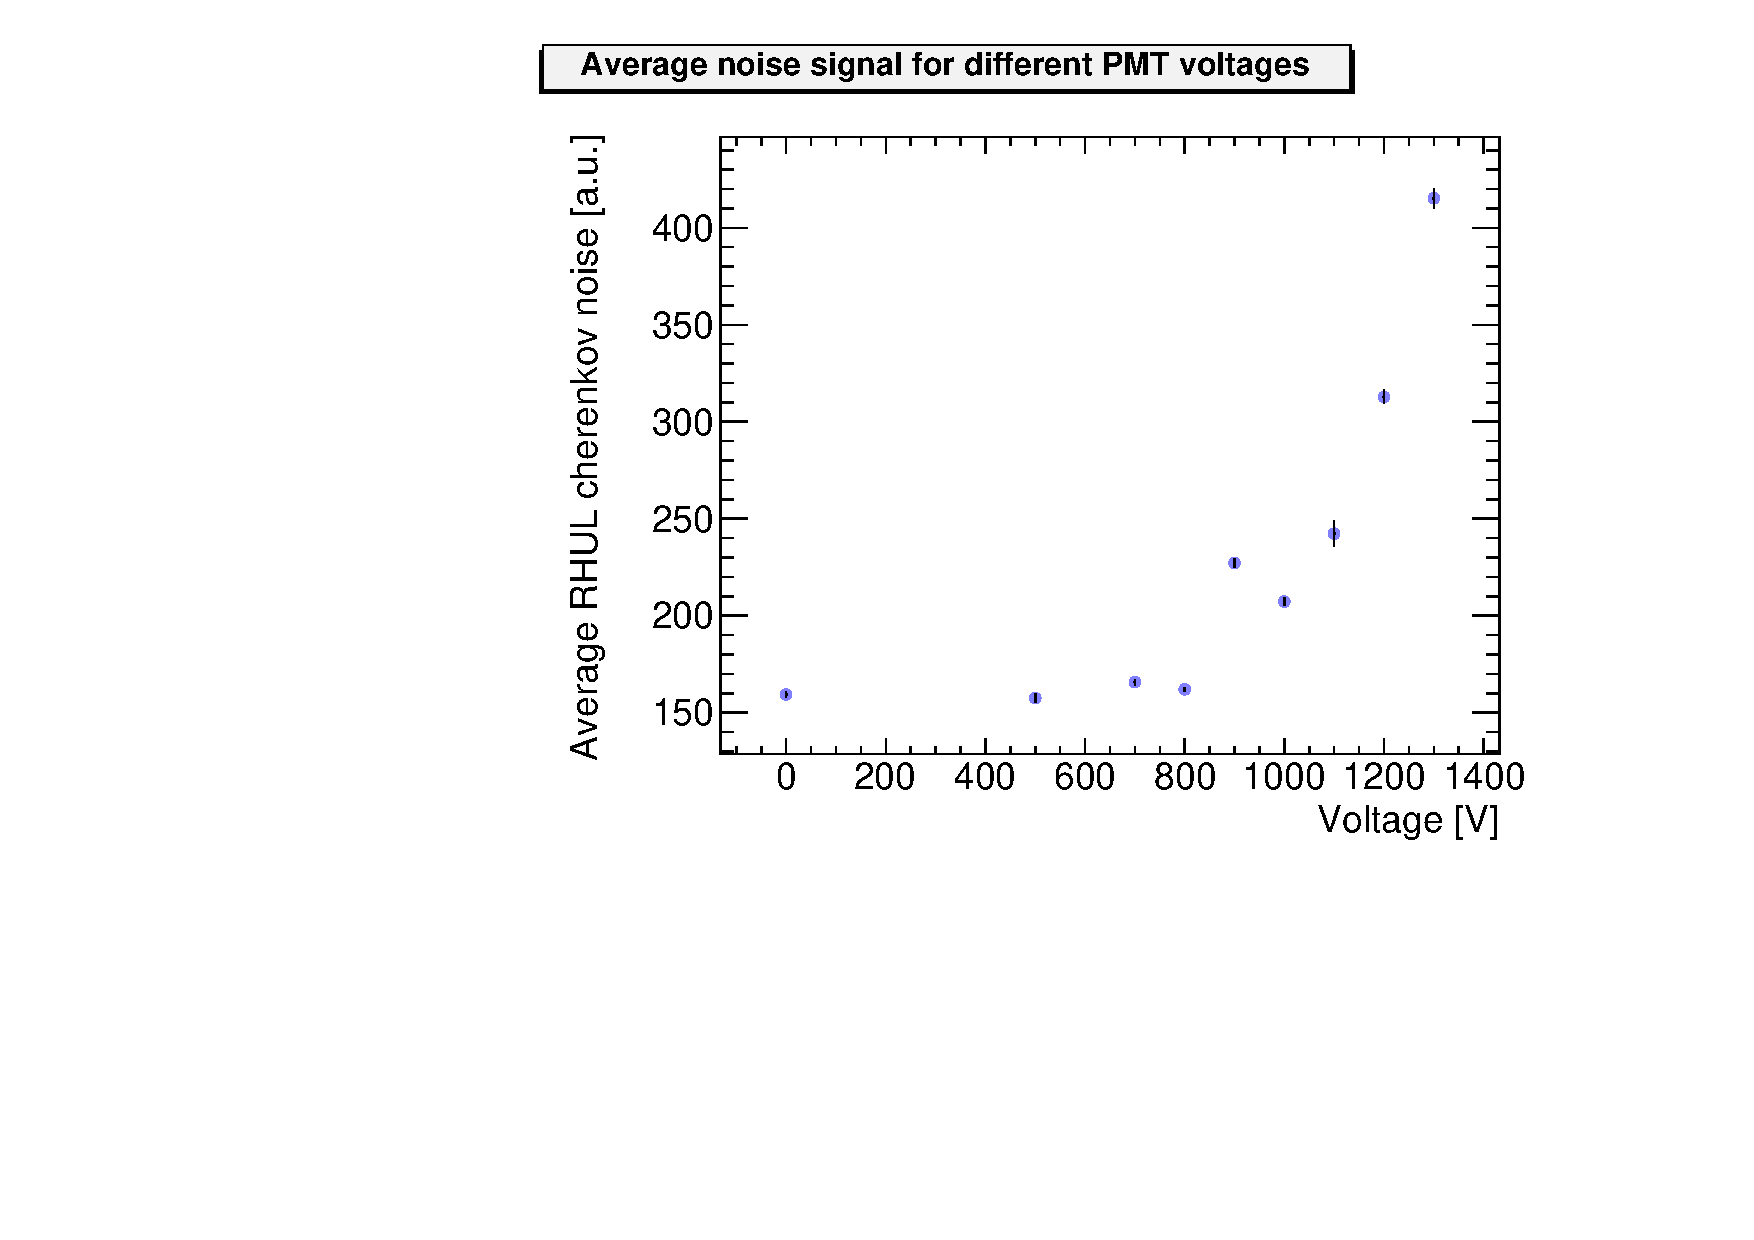
\includegraphics[width=\textwidth]{AverageNoise_perVoltage.pdf}
\caption[RHUL Cherenkov detector noise]{Average noise signal as a function of the voltage applied to the detector PMT. The noise was measured when the ATF beam was turned off. For each voltage, 500 or 1000 ADC pulses of noise were recorded, and the noise averaged over the number of pulses. The error bars to the mean values are the standard deviation of the mean.}
\label{fig:AverageNoise}
\end{figure}
Figure ~\ref{fig:AverageNoise} shows the mean values of the noise measurements for different PMT voltages. For every point either 500 or 1000 ADC pulses were recorded and averaged. The error bars represent the standard deviation on the mean value calculated by $SD=\frac{\sigma}{\sqrt{N}}$, where $\sigma$ is the RMS of the noise distribution at each point and N the number of pulses.\\
At around \SI{800}{\volt} the effect of dark current in the PMT starts getting prominent wherefore the noise rises exponentially. For the data shown in the following, the noise is already subtracted. As the data was taken only for these voltages, for which noise measurements were done, the mean value of noise is subtracted from every signal pulse appropriately. Therefore the rise in noise is automatically taken into account for higher voltages.

\subsubsection{Collimator apertures scan - for different intensities and vacuum pressures}
\label{aperture_scans}
Scans of the background for different collimator apertures were done, first for symmetric positions of the lower and upper jaw around the centre, later for asymmetric positions. Additionally, a scan was done with one jaw fully extracted and the other one moving to certain positions. The last scan is referred to as the 'half aperture scan', whereas the first two scans are the 'symmetric' and the 'asymmetric' scans.\\
Figure ~\ref{fig:AverageSignal_Aperture_BeamIntensities} shows the plot of the average detector signals for the asymmetric scan of different collimator apertures. The scans were done for five different beam intensities. It is clear that the background level rises with increase in intensity. The characteristic shape of the scan is however conserved: the background level is constant while closing the collimator from a full aperture of \SI{24}{\milli\metre} to about \SI{12}{\milli\metre}. When closing to \SI{10}{\milli\metre} the background level drops, and rises again when closing the collimator completely, i.e. to \SI{6}{\milli\metre} full aperture. This characteristic drop and rise between 12 and \SI{6}{\milli\metre} is on the one hand proof of the proper functionality of moving the collimator jaws, on the other hand leaves some questions open: where are the background particles originating that are cut away by the collimator, and does the rise in background mean that the collimator is showering the beam halo particles? Which qualities do these produced background particles have?\\
These questions are addressed in Chapter ~\ref{sec:BDSIM_sim}, in which the effect of the collimator is simulated in a BDSIM simulation.
\newline
Figure~\ref{fig:AverageSignal_Aperture_VacuumPressures} shows a plot of a measurement done in the same way but for two different vacuum pressures: \SI{4.9e-7}{\pascal} and \SI{1.06e-6}{\pascal}. The graphs are directly comparable as they both show data taken for a beam intensity of \num{0.5}$\pm$\num{0.03e10}. It is clear and as expected that the background level is higher for a worse vacuum, i.e. for a higher pressure. Nevertheless, the background level is not only shifted. By closing the collimator to an aperture of \SI{10}{\milli\metre}, the background reduced to almost the same level whereas at the plateau (between 12 and \SI{24}{\milli\metre}) the background level for the smaller pressure is almost double. The collimator reduces therefore the background dramatically, especially at high background rates.

\begin{figure}
\centering
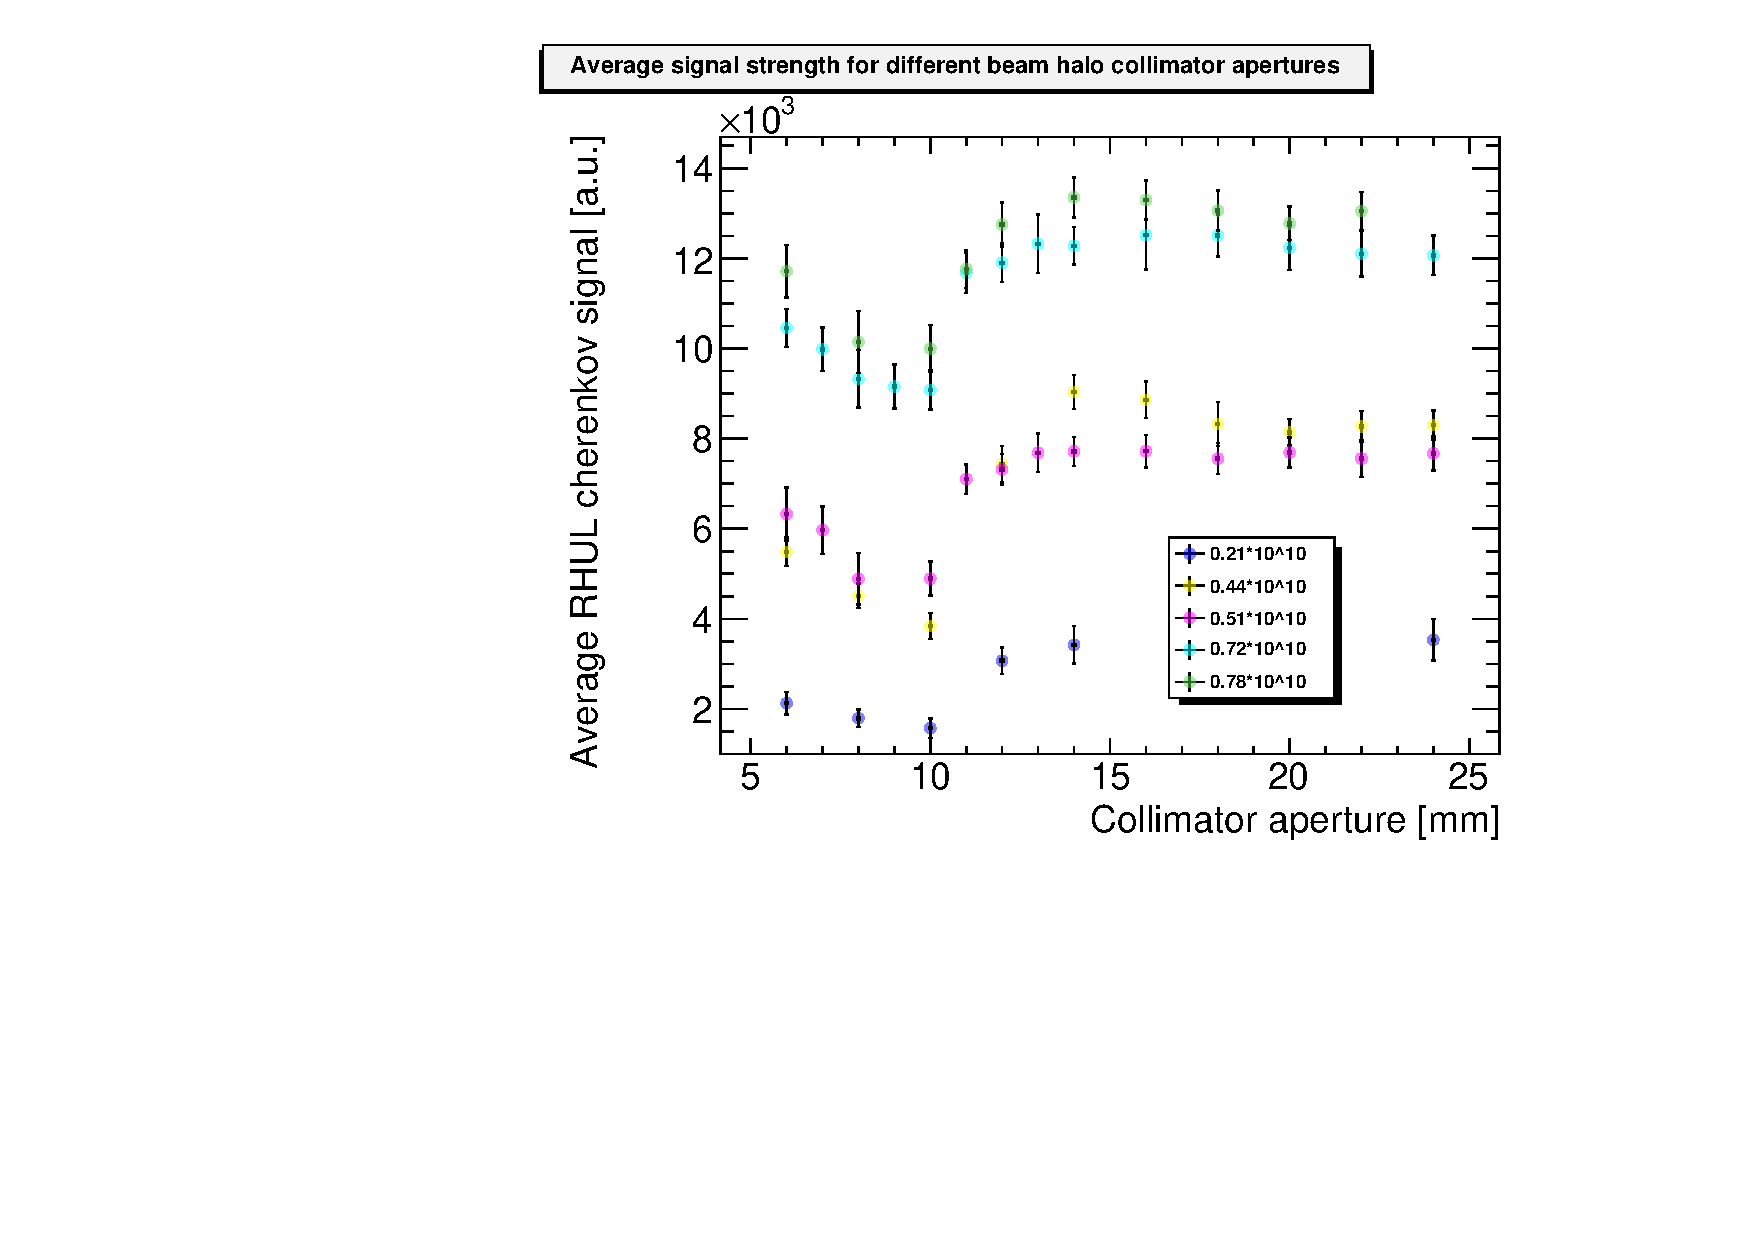
\includegraphics[width=\textwidth]{AverageSignal_perAperture.pdf}
\caption[RHUL Cherenkov detector signal vs. collimator aperture: different beam intensities]{Average signal as a function of the full aperture of the vertical beam halo collimator. The signal was measured for different beam intensities [\num{10e10}]: 0.21$\pm$0.02, 0.44$\pm$0.02, 0.51$\pm$0.02, 0.72$\pm$0.02 and 0.78$\pm$0.02, while the PMT voltage was constant at \SI{900}{\volt}. For each aperture, 500 ADC pulses were recorded, and the signal was averaged over the number of pulses. The error bars to the mean values are the standard deviation of the signal distributions at each point.\\For some scans, the data was not taken for all apertures. Therefore, especially the graph for the beam intensity of \num{0.21}$\pm$\num{0.02e10} is missing data points for the half millimetre steps and between 14 and \SI{24}{\milli\metre}.}
\label{fig:AverageSignal_Aperture_BeamIntensities}
\end{figure}
\begin{figure}
\centering
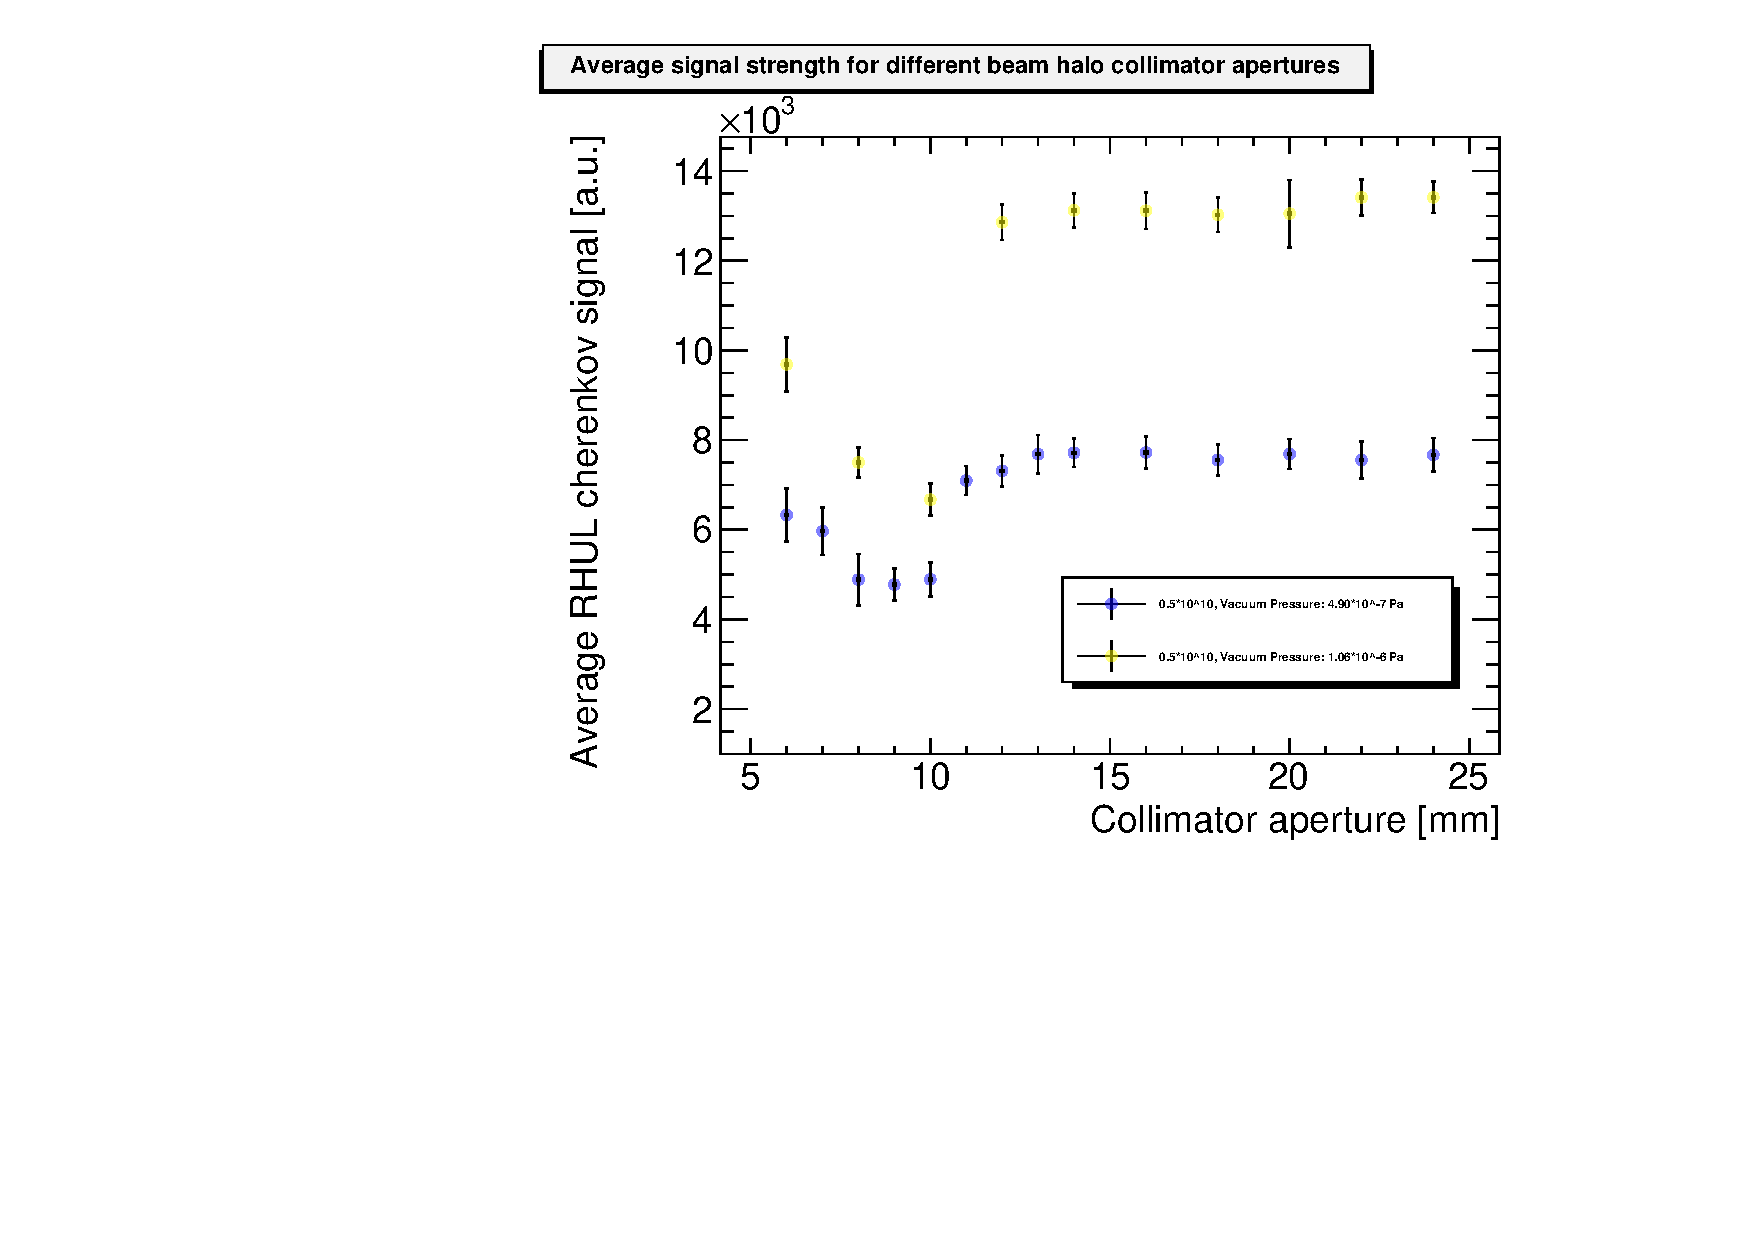
\includegraphics[width=\textwidth]{AverageSignal_perAperture_VacuumPressures.pdf}
\caption[RHUL Cherenkov detector signal vs. collimator aperture: different vacuum pressures]{Average signal as a function of the full aperture of the vertical beam halo collimator. The signal was measured for a beam intensity of \num{0.5}$\pm$\num{0.03e10} and a PMT voltage of \SI{900}{\volt}. The vacuum pressure was lowered from \SI{4.9e-7}{\pascal} to \SI{1.06e-6}{\pascal}. For each aperture, 500 ADC pulses were recorded, and the signal was averaged over the number of pulses. The error bars to the mean values are the standard deviation of the signal distributions at each point.}
\label{fig:AverageSignal_Aperture_VacuumPressures}
\end{figure}

\subsubsection{Test collimator alignment wrt beam position}
\label{collimator_alignment}
The next measurement sets are done to experimentally test whether the collimator is aligned in such a way that the beam is going through the centre between the jaws. The idea is that the background signal should be asymmetric if the beam is closer to one or the other side.\\Figure~\ref{fig:AverageSignal_HalfAperture} shows a plot of a measurement where one of the jaws was moved while the other jaw stayed in the fully extracted position. It is clear that moving the upper jaw shows the same characteristic background shape as before in the plots~\ref{fig:AverageSignal_Aperture_BeamIntensities} and \ref{fig:AverageSignal_Aperture_VacuumPressures}. But moving the lower jaw only shows no significant change in background. This leaves one with the possible conclusion that the beam is not in the centre between the two jaws but rather closer to the upper jaw. One could then say that also the background shape of the previous plots are only influenced by the upper jaw only. To confirm this conclusion, more measurements of this kind should be done to exclude a statistical fluctuation or simply a mistake in the process of data taking.
\newline
The next four figures show scans with asymmetric jaw positions around a certain value, i.e. 4 or \SI{5}{\milli\metre}. For each value, around which the jaws were moved, two measurements were done for the intensities of \num{0.84}$\pm$\num{0.03e10} and \num{1.01}$\pm$\num{0.03e10}. The plots are showing the background level in dependency of the position of the upper and lower jaw. As one jaw was moved in, the other one was simultaneously moved out, because of which the data line is diagonal in the diagrams. In all of the plots the drop in background level is clearly visible for a upper jaw position of \SI{5}{\milli\metre}, which follows the same behaviour as before. By closing the jaw more, the background level rises again and peaks for the minimal upper jaw position as the collimator jaw moves into the beam. All this seems to be consistent with the assumption that also here the lower jaw doesn't effect the beam in any way. Otherwise the plot would also show low background intensities for lower jaw positions of below \SI{5}{\milli\metre} which is not the case.\\
Especially significant is Figure~\ref{fig:AverageSignal_Asymmetric_5mm_101} with an identical background behaviour as in the measurements in Section~\ref{aperture_scans}. Also here it would be easier to make meaningful statements if the measurements would have more data points for larger jaw position regions, especially for the same positions in all plots.
\begin{figure}
\centering
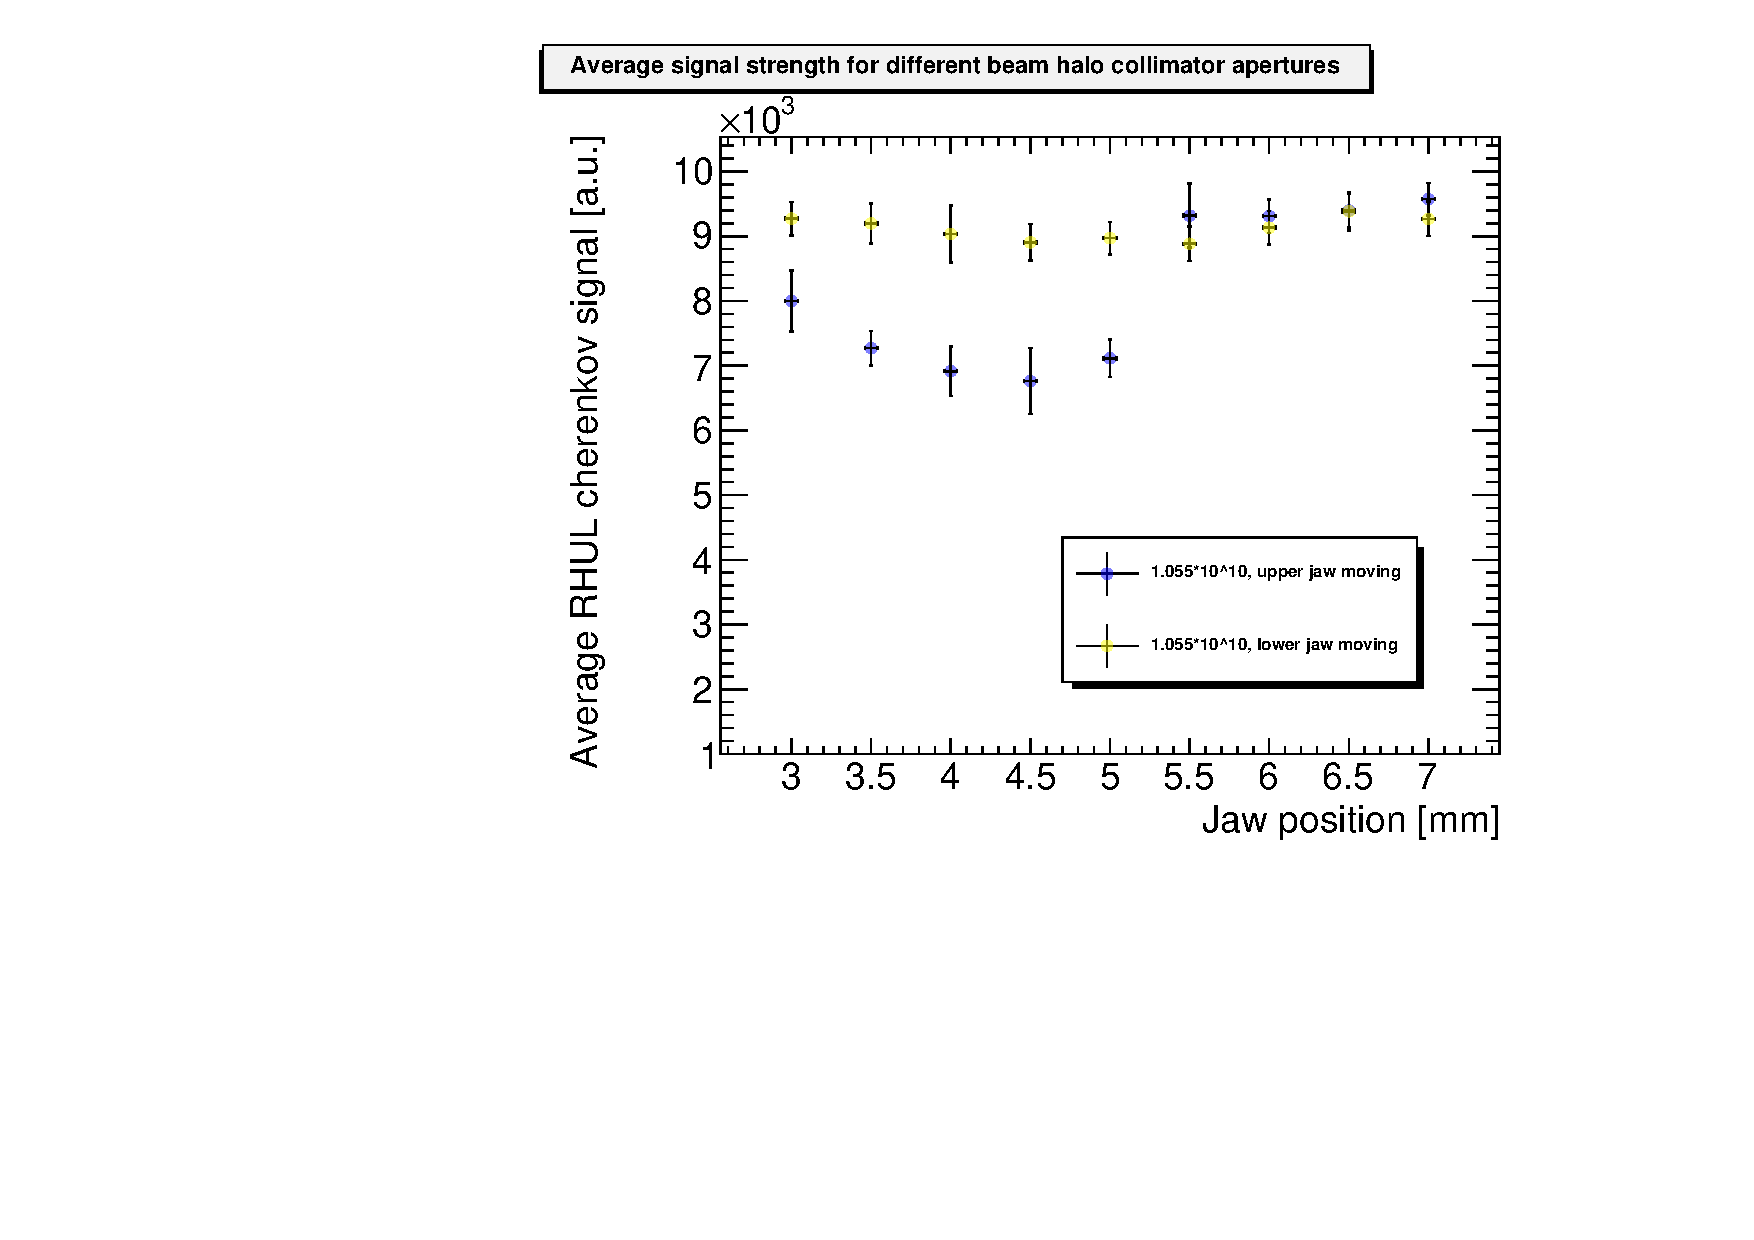
\includegraphics[width=\textwidth]{AverageSignal_perJawPosition.pdf}
\caption[RHUL Cherenkov detector signal vs. collimator half aperture]{Average signal as a function of the position of the upper/lower jaw of the vertical beam halo collimator. The signal was measured for a beam intensity of \num{1.05}$\pm$\num{0.04e10} and a PMT voltage of \SI{800}{\volt}. First, the lower jaw was fixed to its open position (\SI{12}{\milli\metre}) and the upper jaw was moved to the positions plotted, then vice versa. For each jaw position, 500 ADC pulses were recorded, and the signal was averaged over the number of pulses. The error bars to the mean values are the standard deviation of the signal distributions at each point.}
\label{fig:AverageSignal_HalfAperture}
\end{figure}
\begin{figure}
\begin{subfigure}[b]{0.5\textwidth}
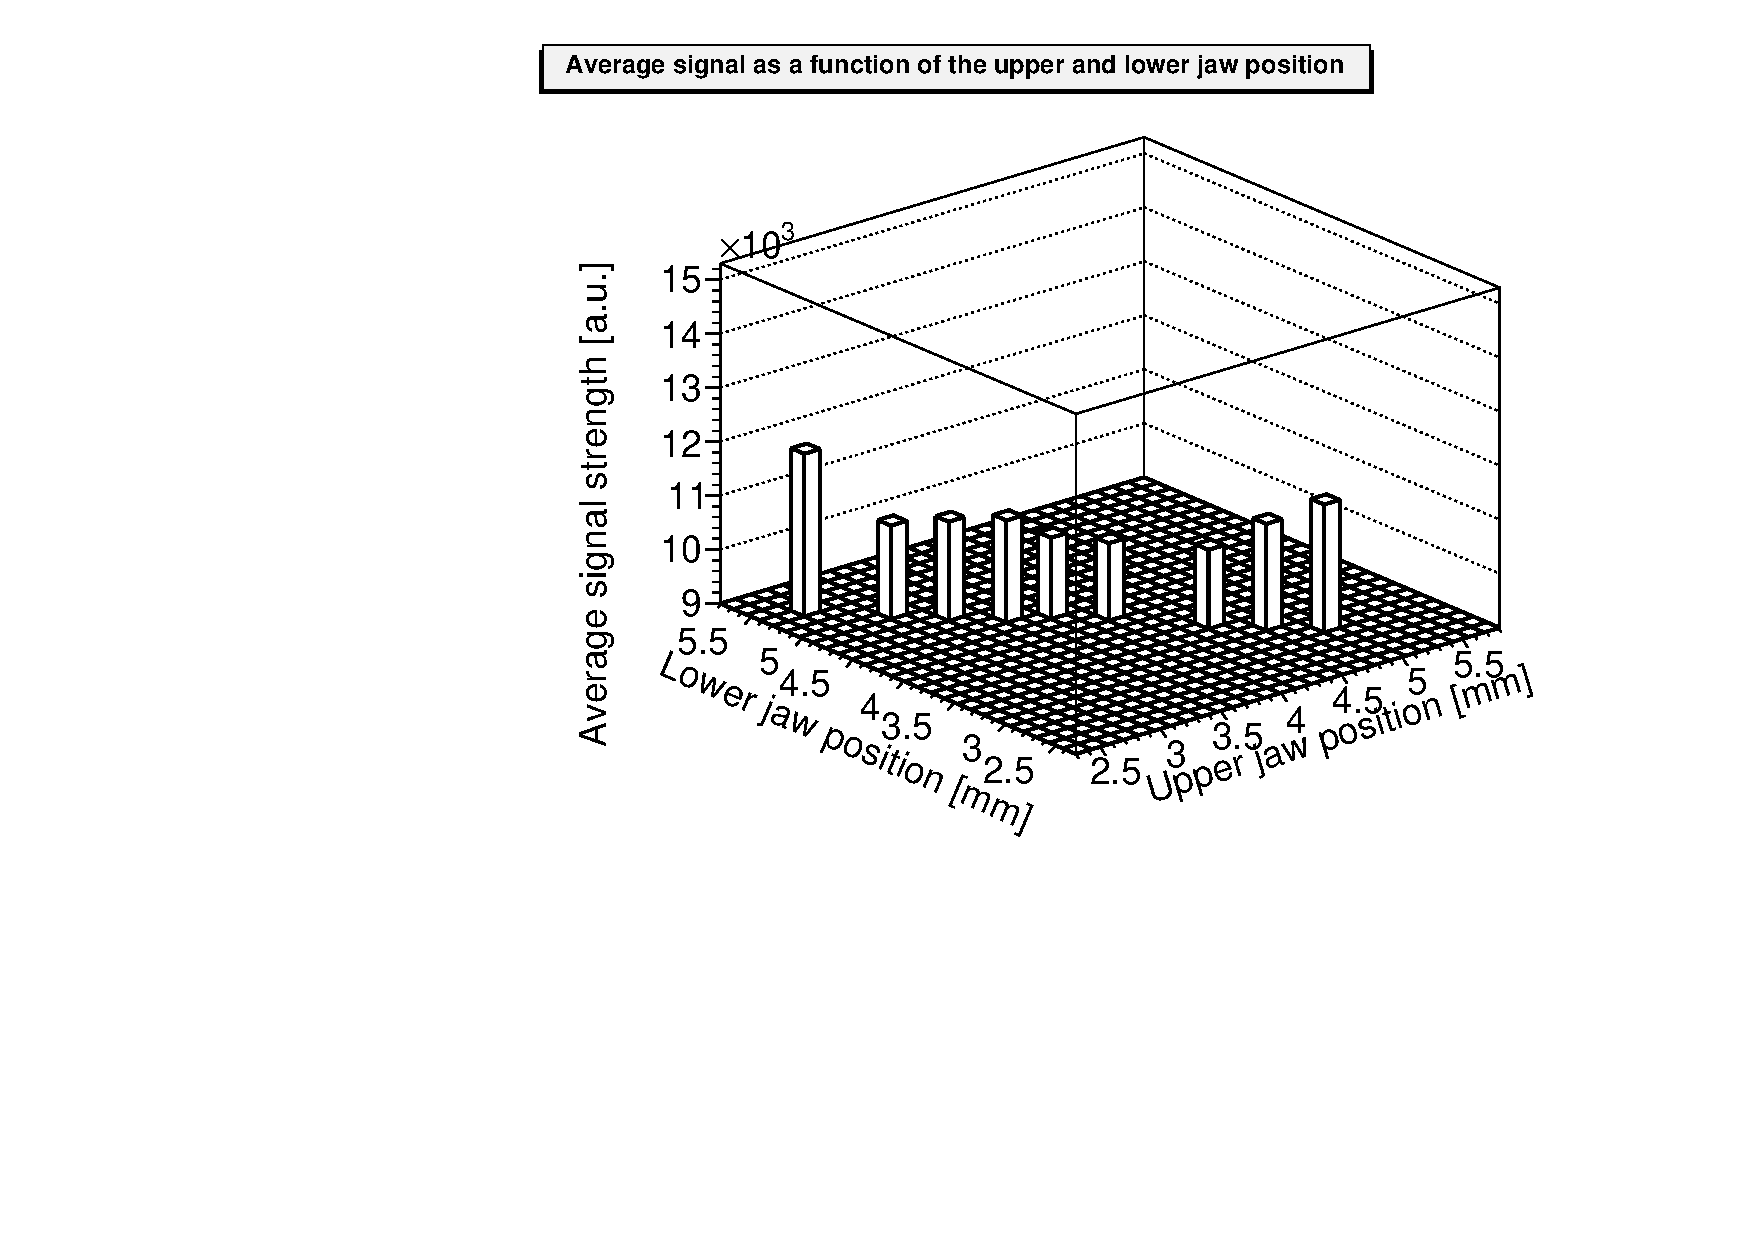
\includegraphics[width=\textwidth]{AsymmetricScan_4mm_beamintensity084_lego.pdf}
\end{subfigure}
\begin{subfigure}[b]{0.5\textwidth}
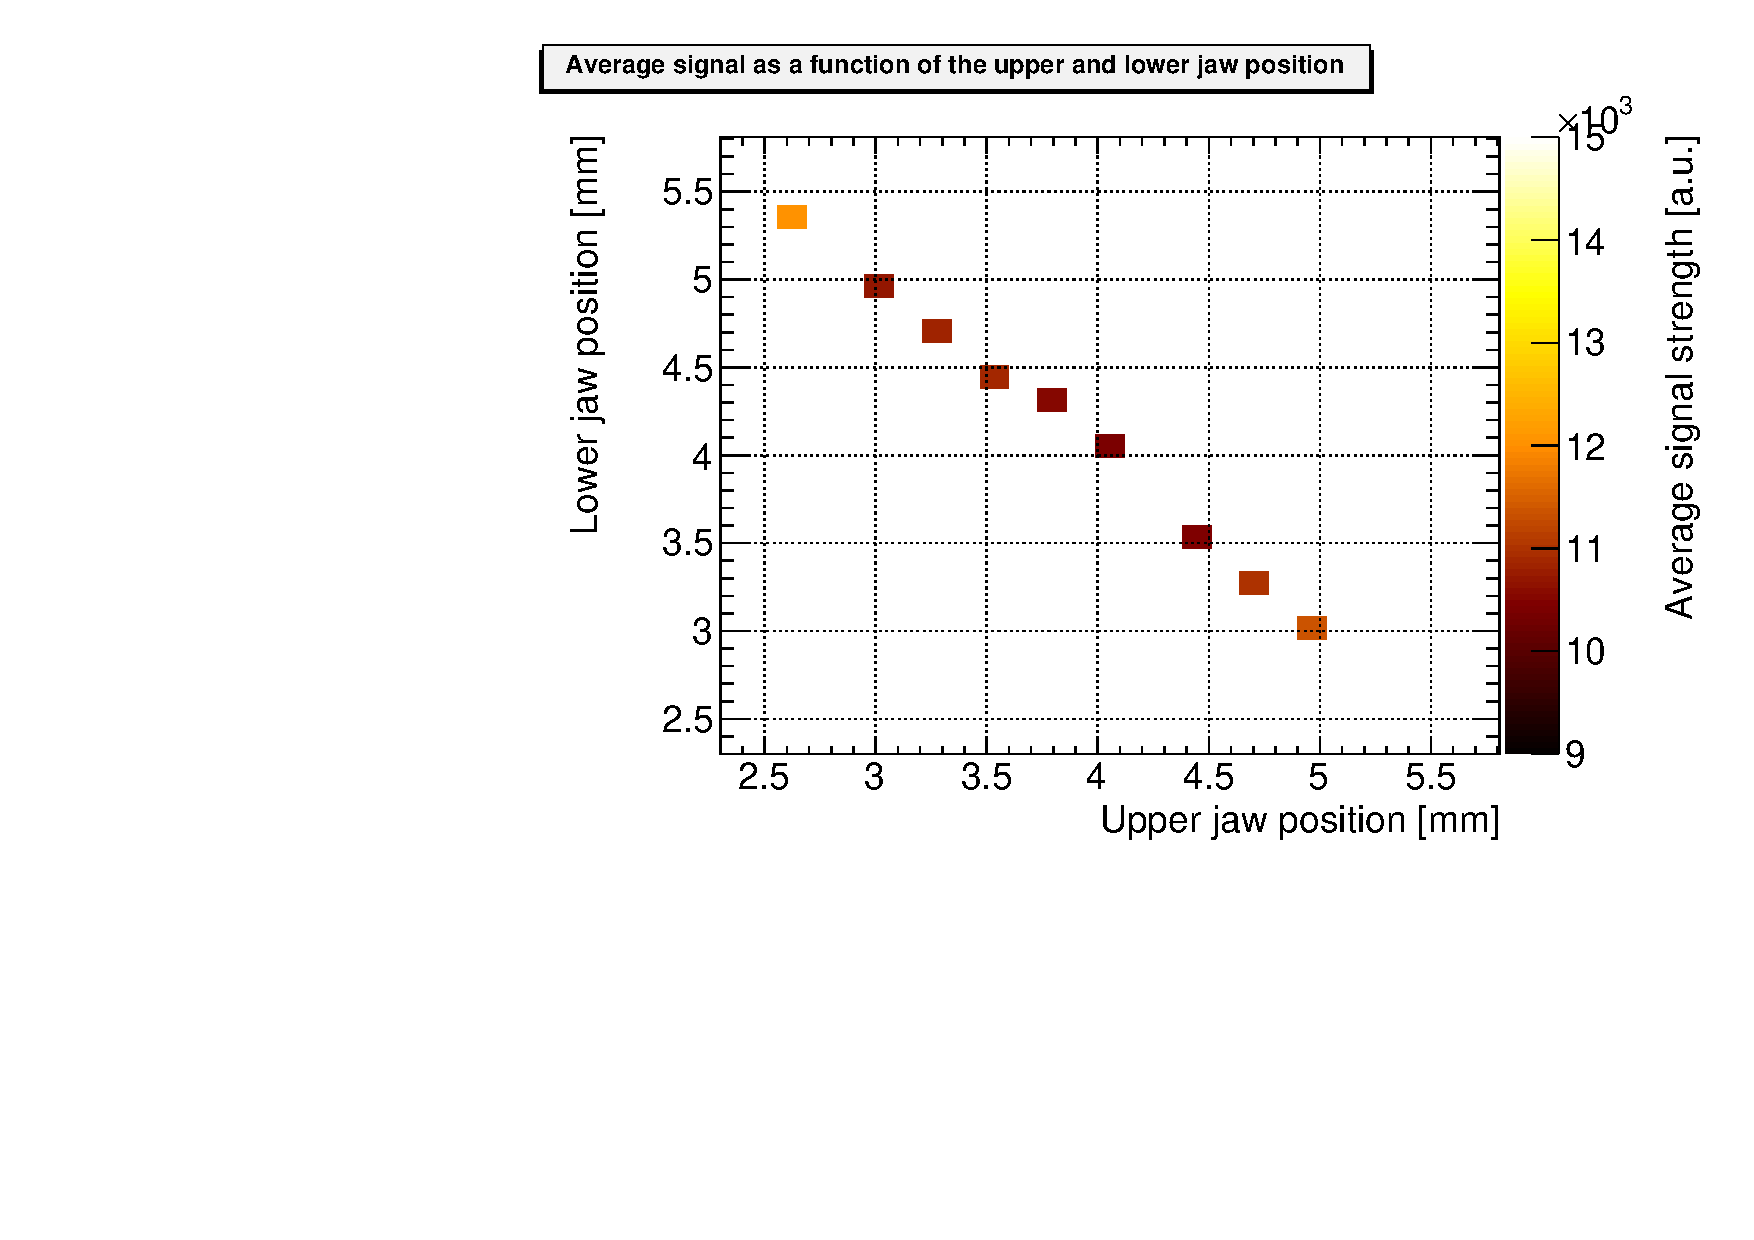
\includegraphics[width=\textwidth]{AsymmetricScan_4mm_beamintensity084_colz.pdf}
\end{subfigure}
\caption[RHUL Cherenkov detector signal for certain upper/lower jaw positions around \SI{4}{\milli\metre}, for a beam intensity of \num{0.84}$\pm$\num{0.03e10}]{Average signal as a function of the position of the upper and lower jaw of the vertical beam halo collimator. The signal was measured for a beam intensity of \num{0.84}$\pm$\num{0.03e10} and a PMT voltage of \SI{900}{\volt}. The jaws were moved simultaneously around \SI{4}{\milli\metre}. For each jaw position, at least 500 ADC pulses were recorded, and the signal was averaged over the number of pulses. The content of the bins were set to the appropriate average signal strength at that point.}
\label{fig:AverageSignal_Asymmetric_4mm_084}
\end{figure}
\begin{figure}
\begin{subfigure}[b]{0.5\textwidth}
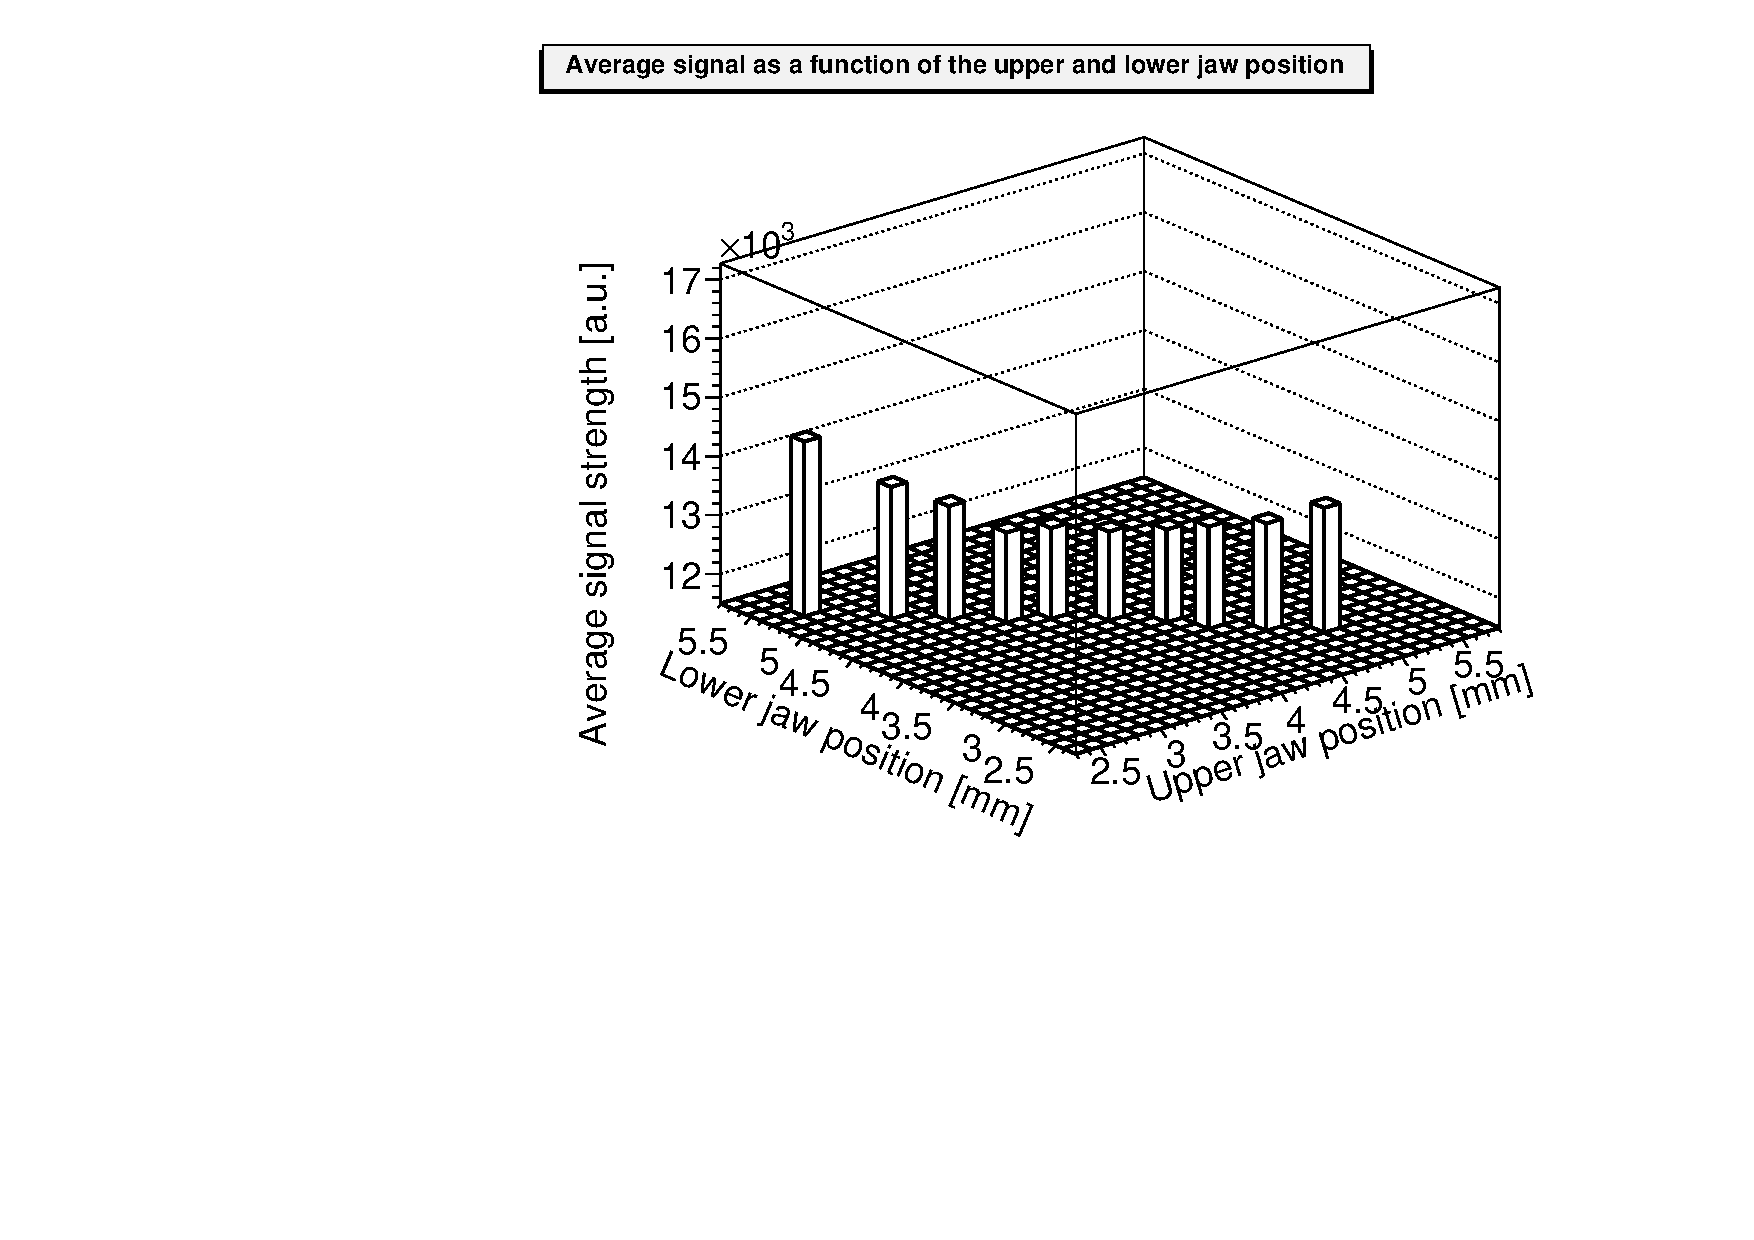
\includegraphics[width=\textwidth]{AsymmetricScan_4mm_beamintensity101_lego.pdf}
\end{subfigure}
\begin{subfigure}[b]{0.5\textwidth}
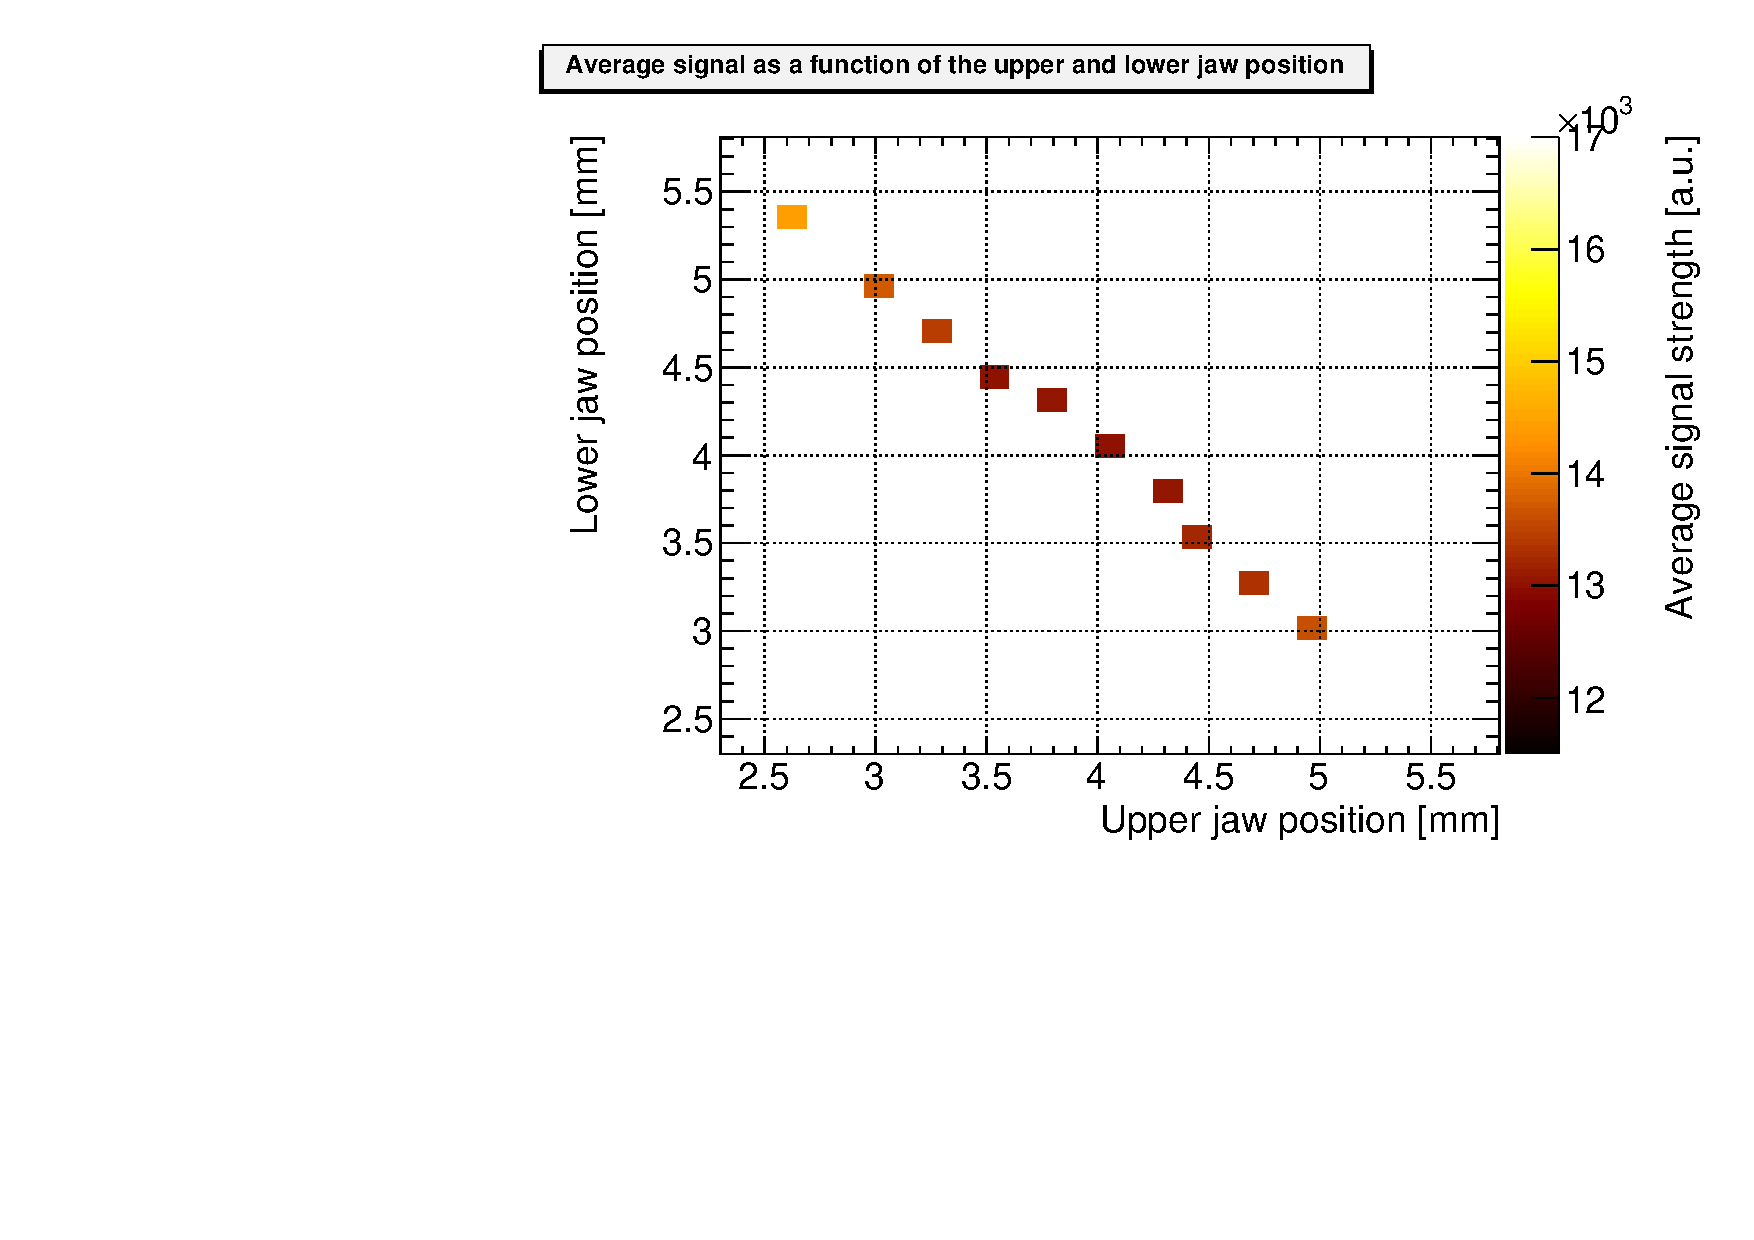
\includegraphics[width=\textwidth]{AsymmetricScan_4mm_beamintensity101_colz.pdf}
\end{subfigure}
\caption[RHUL Cherenkov detector signal for certain upper/lower jaw positions around \SI{4}{\milli\metre}, for a beam intensity of \num{1.01}$\pm$\num{0.03e10}]{Average signal as a function of the position of the upper and lower jaw of the vertical beam halo collimator. The signal was measured for a beam intensity of \num{1.01}$\pm$\num{0.03e10} and a PMT voltage of \SI{900}{\volt}. The jaws were moved simultaneously around \SI{4}{\milli\metre}. For each jaw position, at least 500 ADC pulses were recorded, and the signal was averaged over the number of pulses. The content of the bins were set to the appropriate average signal strength at that point.}
\label{fig:AverageSignal_Asymmetric_4mm_101}
\end{figure}
\begin{figure}
\begin{subfigure}[b]{0.5\textwidth}
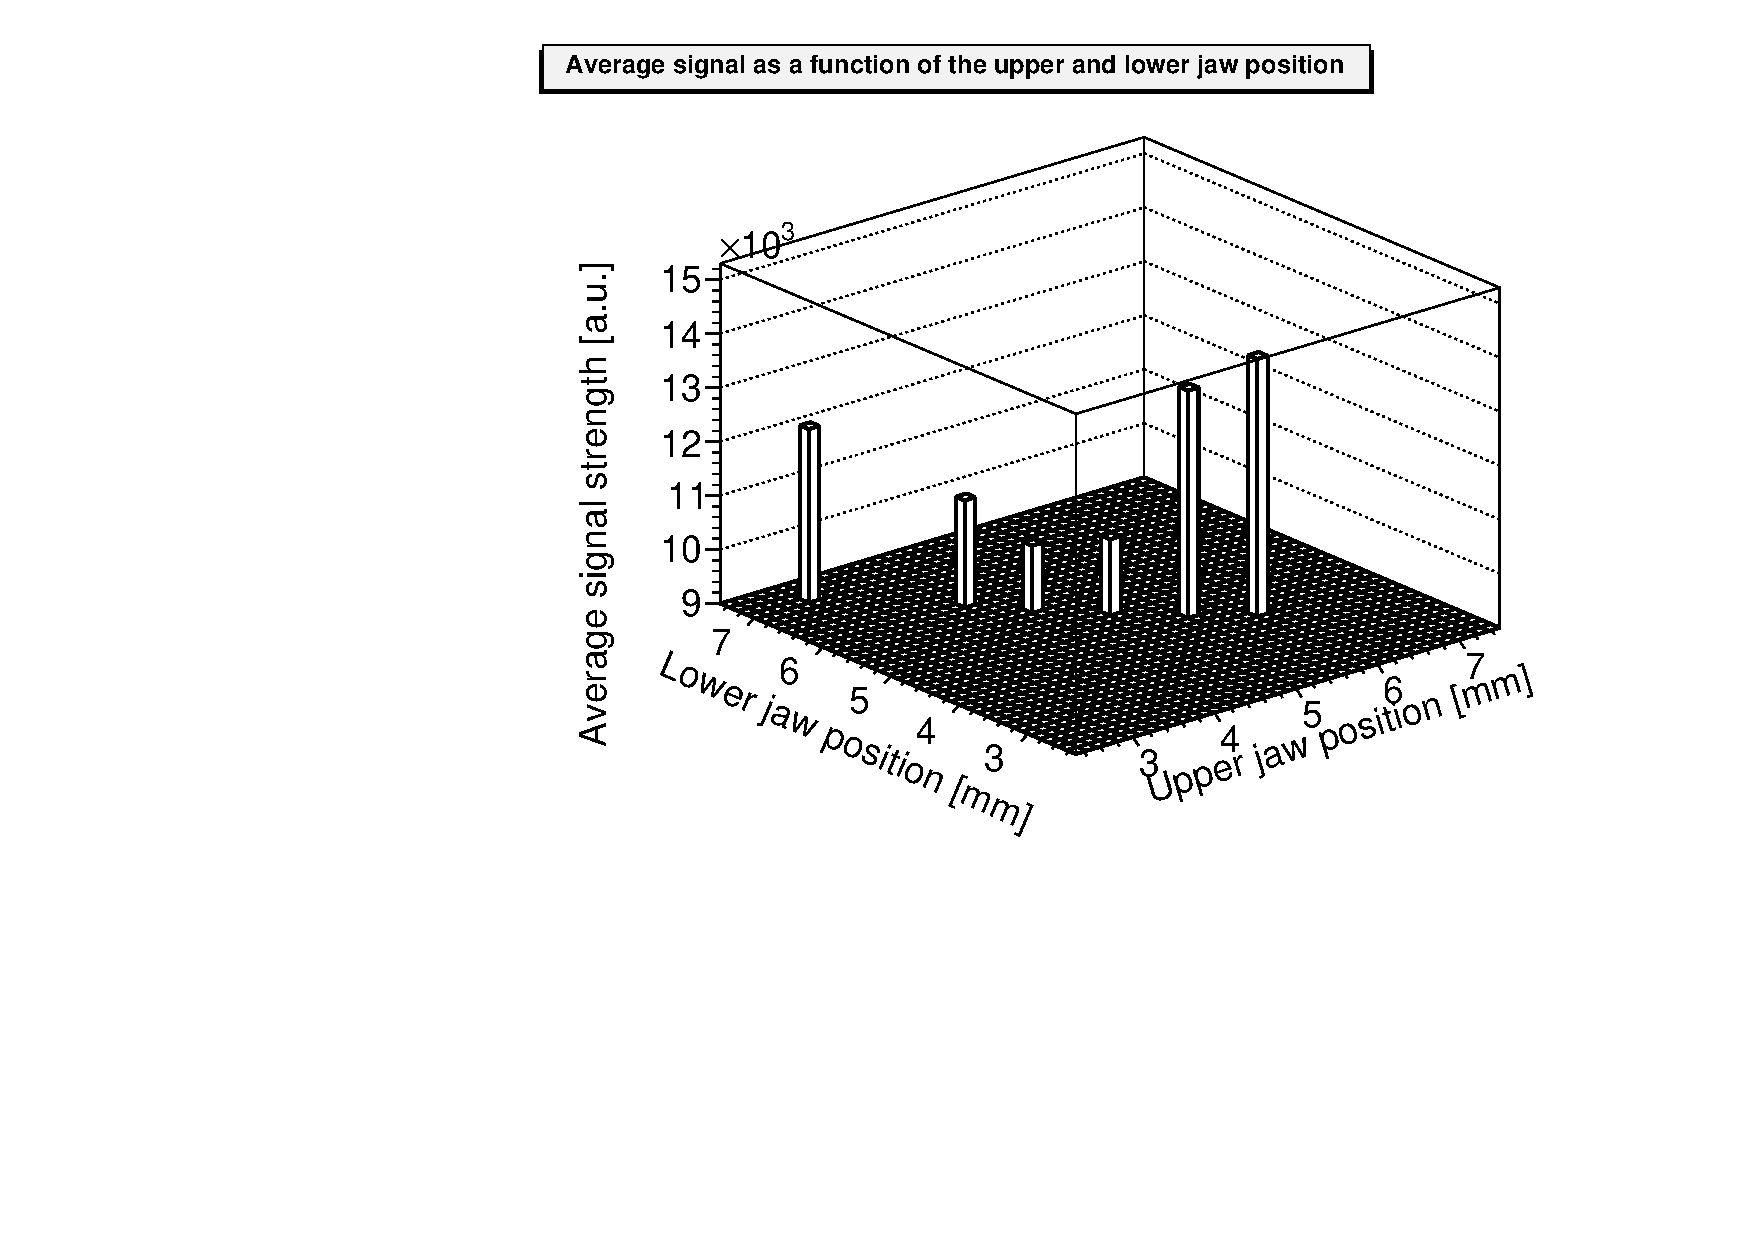
\includegraphics[width=\textwidth]{AsymmetricScan_5mm_beamintensity084_lego.pdf}
\end{subfigure}
\begin{subfigure}[b]{0.5\textwidth}
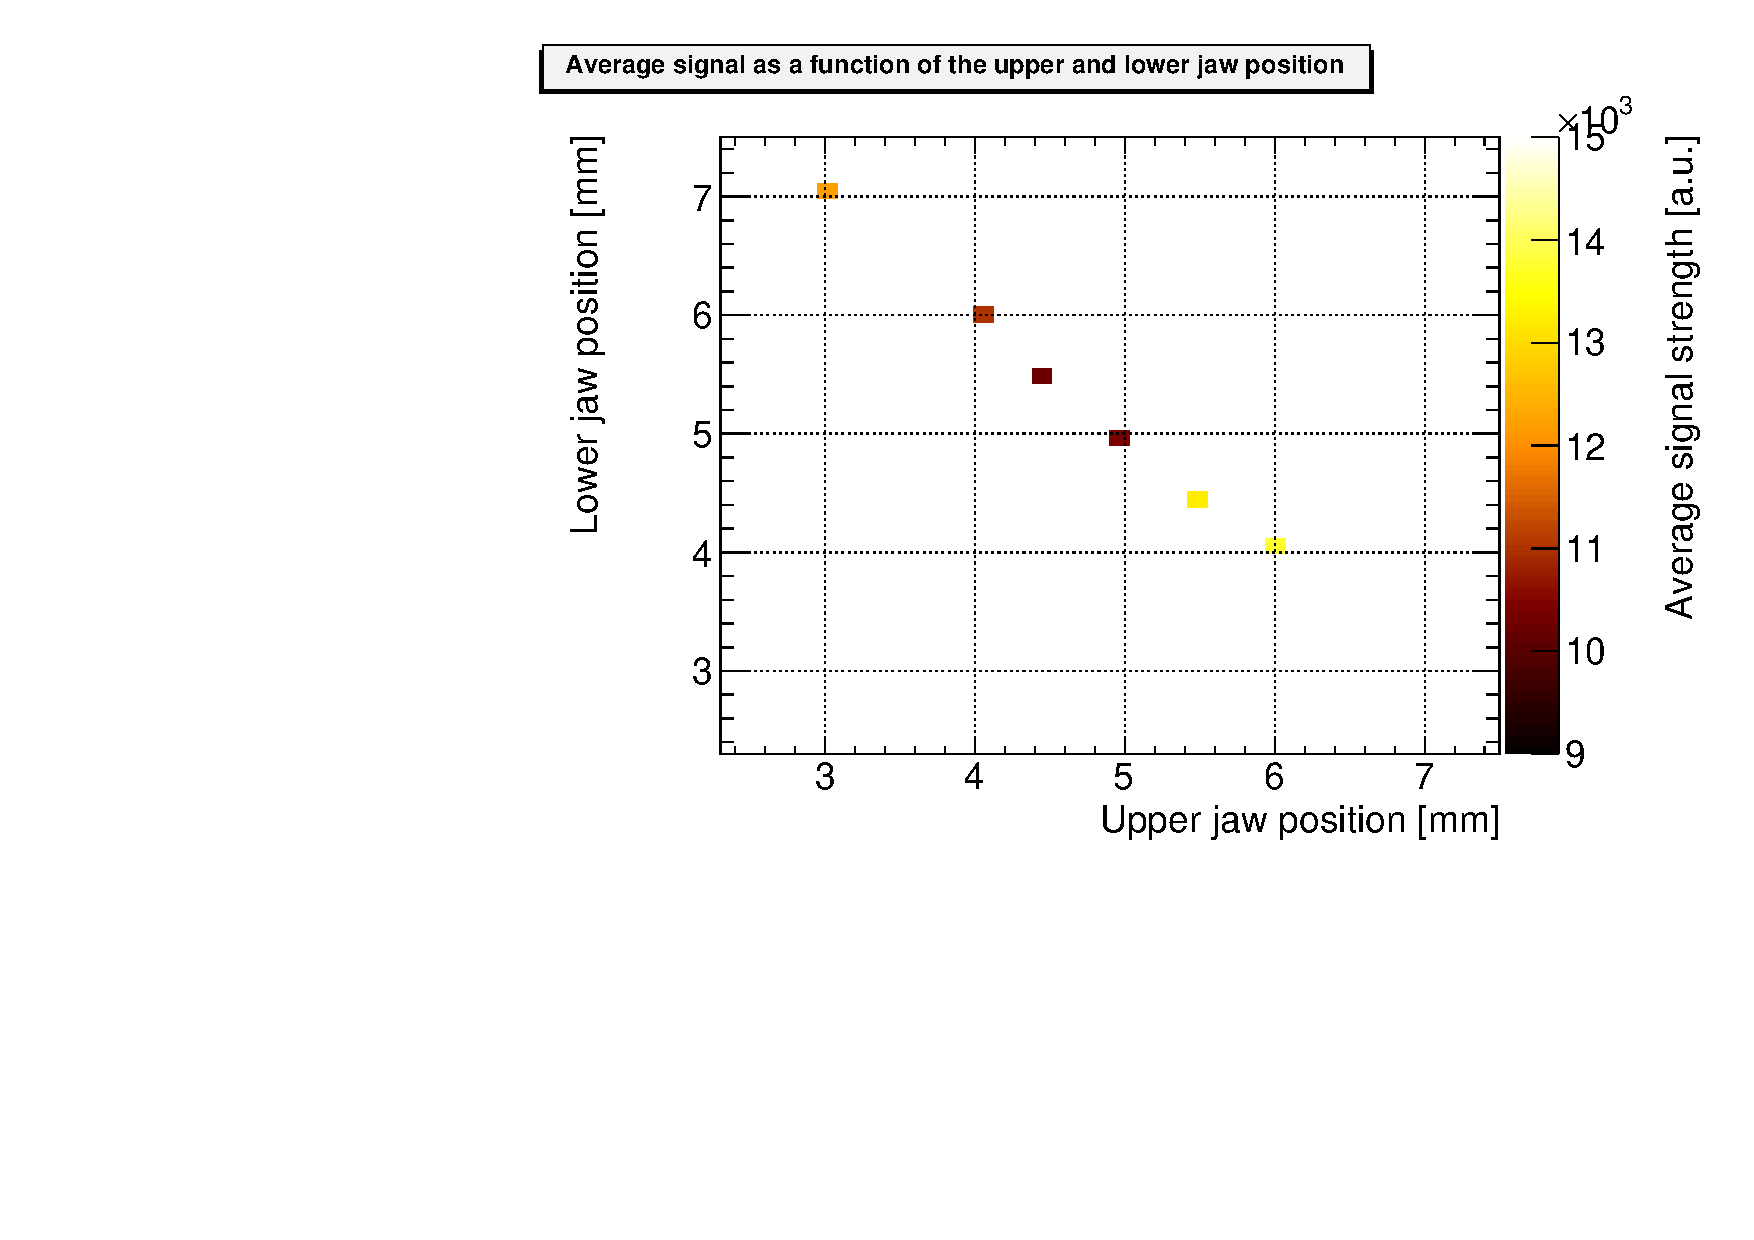
\includegraphics[width=\textwidth]{AsymmetricScan_5mm_beamintensity084_colz.pdf}
\end{subfigure}
\caption[RHUL Cherenkov detector signal for certain upper/lower jaw positions around \SI{5}{\milli\metre}, for a beam intensity of \num{0.84}$\pm$\num{0.03e10}]{Average signal as a function of the position of the upper and lower jaw of the vertical beam halo collimator. The signal was measured for a beam intensity of \num{0.84}$\pm$\num{0.03e10} and a PMT voltage of \SI{900}{\volt}. The jaws were moved simultaneously around \SI{5}{\milli\metre}. For each jaw position, at least 500 ADC pulses were recorded, and the signal was averaged over the number of pulses. The content of the bins were set to the appropriate average signal strength at that point.}
\label{fig:AverageSignal_Asymmetric_5mm_084}
\end{figure}
\begin{figure}
\begin{subfigure}[b]{0.5\textwidth}
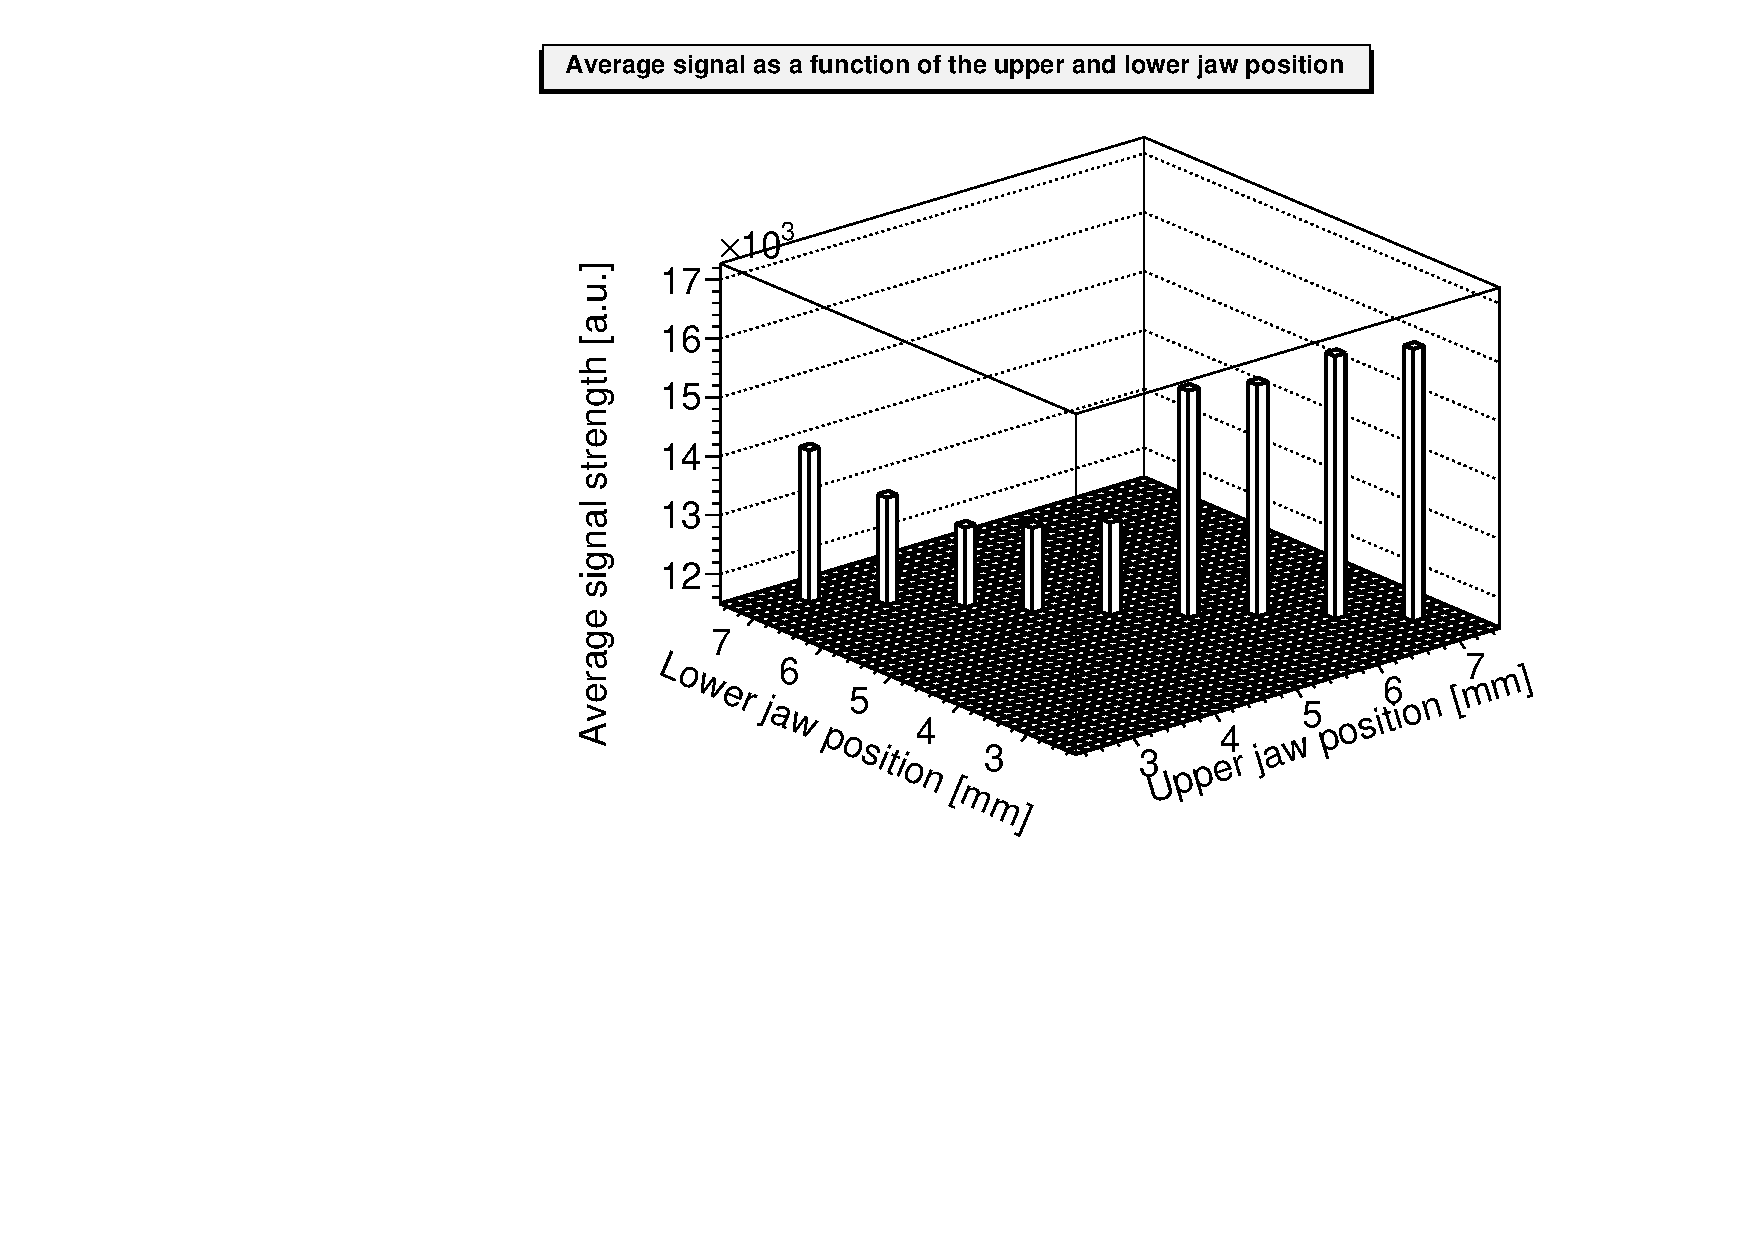
\includegraphics[width=\textwidth]{AsymmetricScan_5mm_beamintensity101_lego.pdf}
\end{subfigure}
\begin{subfigure}[b]{0.5\textwidth}
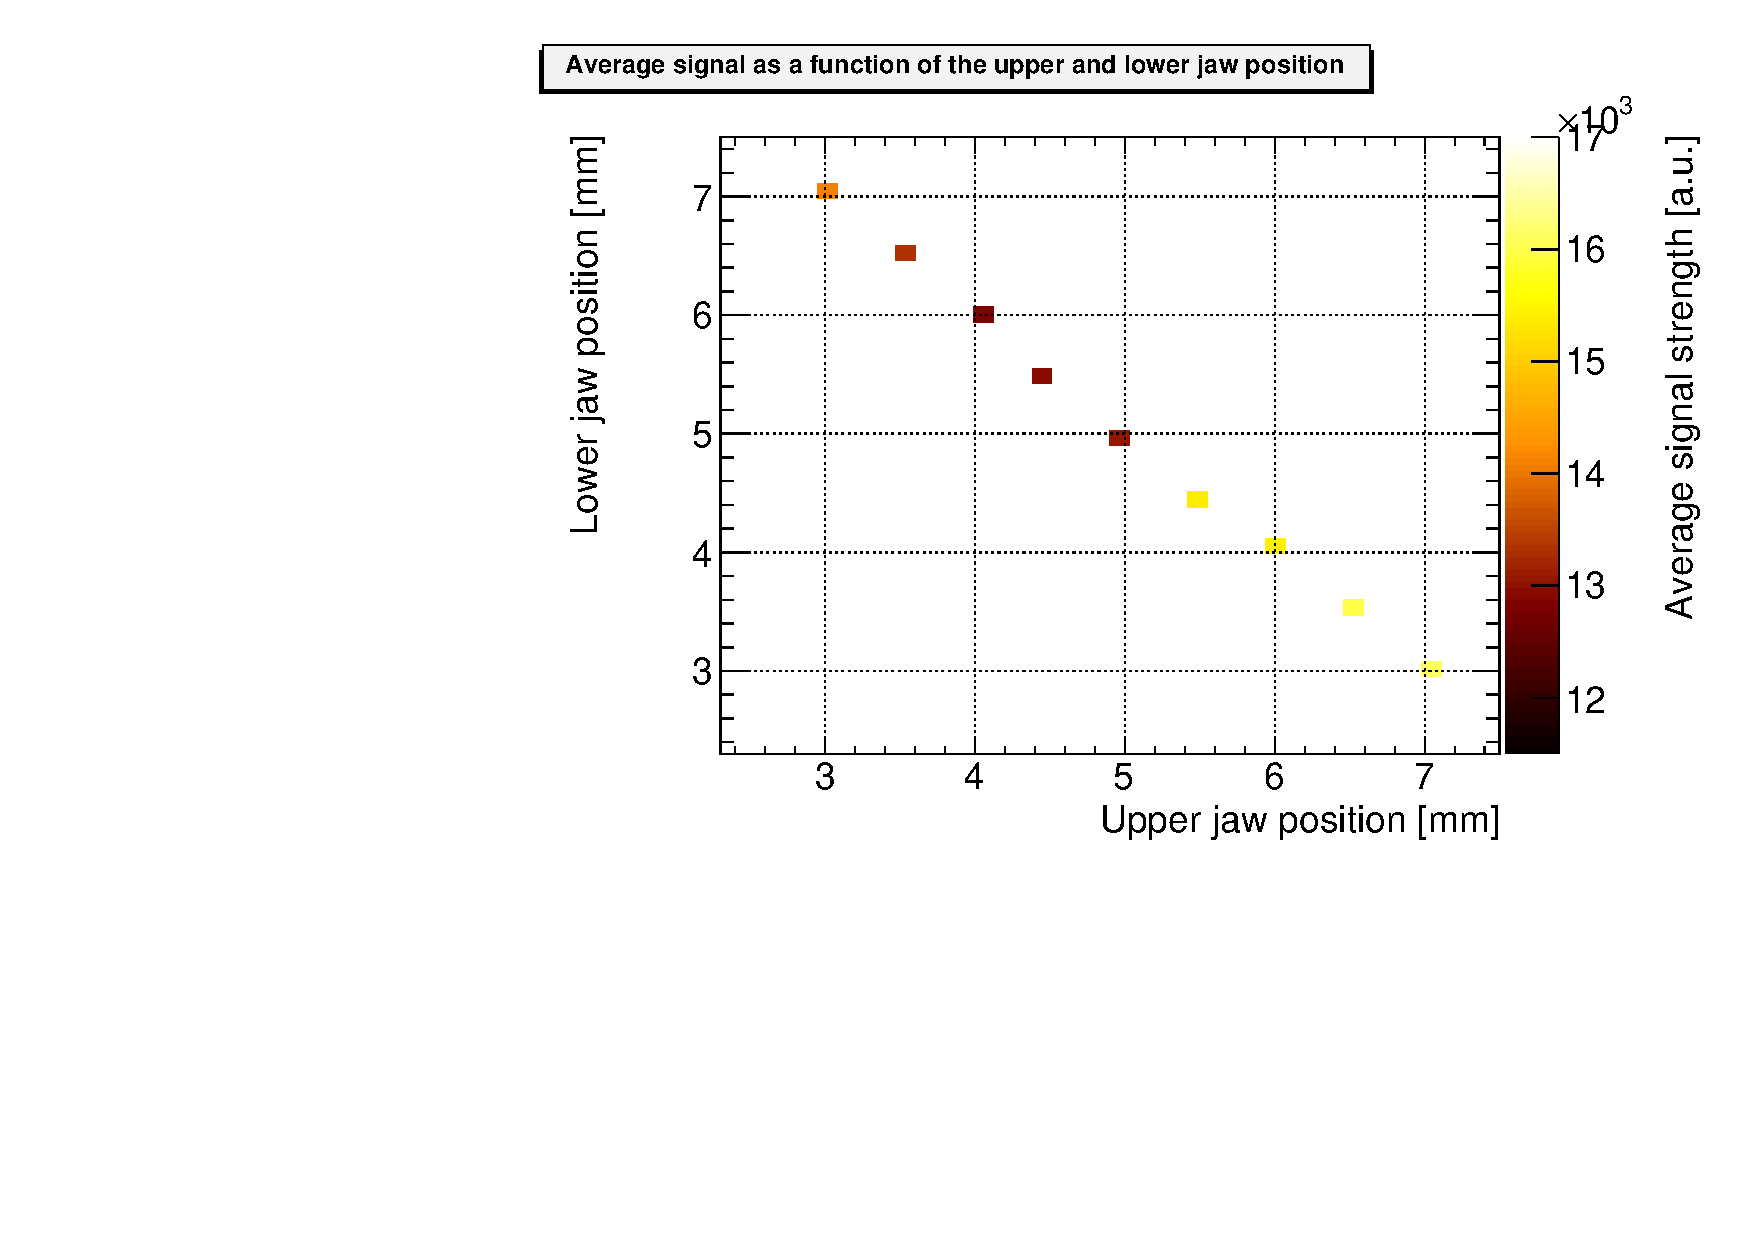
\includegraphics[width=\textwidth]{AsymmetricScan_5mm_beamintensity101_colz.pdf}
\end{subfigure}
\caption[RHUL Cherenkov detector signal for certain upper/lower jaw positions around \SI{5}{\milli\metre}, for a beam intensity of \num{1.01}$\pm$\num{0.03e10}]{Average signal as a function of the position of the upper and lower jaw of the vertical beam halo collimator. The signal was measured for a beam intensity of \num{1.01}$\pm$\num{0.03e10} and a PMT voltage of \SI{900}{\volt}. The jaws were moved simultaneously around \SI{5}{\milli\metre}. For each jaw position, at least 500 ADC pulses were recorded, and the signal was averaged over the number of pulses. The content of the bins were set to the appropriate average signal strength at that point.}
\label{fig:AverageSignal_Asymmetric_5mm_101}
\end{figure}
%---------------------------------------------------
\subsection{Collimator as background source}
\label{sec:BDSIM_sim}
As the data in the figures in the two previous sections have shown, the collimator reduces the existing background level if closed to an aperture of \SI{10}{\milli\metre}. By closing the jaws further, the background level increases again. The questions where this already existing background is coming from, and how the background is increased by the jaws driven into the beam, are now addresses by the following plots showing data from \bdsim simulations of the ATF2 lattice.

\subsection{Effect on background level at IP}
\label{collimator_bkg_IP}
We have seen that the background level around the collimator area is dramatically affected by the movement of the collimator jaws. However, the actual effect of the collimator on the background level at the interaction point might be different, and is now discussed.

%---------------------------------------------------
\section{Background from a Muon Spoilers}
\subsection{MUCARLO}

\chapter{Background from Beam Dumps}
\label{BeamDumps}
\section{FLUKA}
\label{BeamDumps:fluka}
\section{Beam dump design}
\label{BeamDumps:design}
\section{EXT line lattice}
\label{BeamDumps:lattice}
\section{Simulation studies of neutrons reaching the IR}
\label{BeamDumps:simulation}

\chapter{Impact of the discussed Background Sources on the Detectors for different scenarios}
\label{EffectDetectors}
The previous chapters introduced and discussed studies of several different background sources that occur at a linear collider.
The impact that these background sources have on the detectors will be discussed in detail for different scenarios.
First, the results for nominal ILC beam and machine parameters will be presented, followed by the results for different beam orbit specifications.
In the end, it will be shown that also different machine parameters have different effects on the outcome.

\section{Results for nominal beam and machine parameters}
\label{EffectDetectors:Nominal}
\subsection{Hit maps of the SiD subdetectors}
\label{EffectDetectors:hitmaps}
\subsection{Occupancy studies and buffer depth}
\label{EffectDetectors:occupancy}
\subsection{Hit time distributions}
\label{EffectDetectors:hittime}
\subsection{Resulting Dosis of the detectors}
\label{EffectDetectors:dosis}

\section{Results for different beam orbit specifications}
\label{EffectDetectors:BeamOrbit}

\subsection{Beam orbit deviating from the ideal nominal specifications}
\label{EffectDetectors:BeamOrbit:otherspecs}
\subsection{Resulting Dosis of the detectors}
\label{EffectDetectors:BeamOrbit:dosis}

\section{Results for different machine parameters}
\label{EffectDetectors:MachineParameters}
\subsection{Continuous wave mode}
\label{EffectDetectors:MachineParameters:CW}
In the Continuous Wave (CW) mode, the particle beam is accelerated by an electromagnetic continuous wave with constant amplitude and frequency.
\subsection{Beam pipe radius}
\label{EffectDetectors:MachineParameters:beampipe}
\subsection{Bunch spacings}
\label{EffectDetectors:MachineParameters:bunchspacing}
\subsection{TeV-Upgrade}
\label{EffectDetectors:MachineParameters:upgrade}
\subsection{Resulting Dosis of the detectors}
\label{EffectDetectors:MachineParameters:dosis}


\chapter{Prospects, Requirements and Limits for a Future Linear Collider}
\label{Results}

As chapter~\ref{EffectDetectors} has shown, the background sources of a linear collider are dependent on the certain factors, like the beam orbit and the machine parameters.
These dependencies result in requirements and limits that can be formulated for the International Linear Collider.
\chapter{Conclusion}
\label{Conclusion}


\begin{appendix}                              %%% start the appendix for longer calculations/info
\documentclass[xcolor={dvipsnames}]{beamer}
\usepackage{color, colortbl}
\usepackage[ngerman,english]{babel}
\usepackage[T1]{fontenc}
\usepackage{CJKutf8} %japanese
\usepackage{lmodern}
%\usepackage{subfigure}
\usepackage[compatibility=false]{caption}
\usepackage{subcaption}
\usepackage{tikz}
\usepackage{textgreek}
\usepackage{tabularx}
\usepackage{ragged2e}
\usepackage{adjustbox}
\usepackage{booktabs}
\usepackage{siunitx}
\usepackage{units}
\usepackage{appendixnumberbeamer}
\usepackage[absolute,overlay]{textpos} %for positioning the logos where I want

\usepackage{animate}
\usepackage{multimedia}
\usepackage{fixltx2e}
\usepackage{multicol}
\usepackage{comment}
\DeclareSIUnit\year{yr}

\mode<presentation>
{
  \usetheme{CambridgeUS}     
  \usecolortheme{lily} 
  \definecolor{beamer@violet}{rgb}{0.5,0.3,0.5} % changed this
  \setbeamercolor{structure}{fg=beamer@violet!70!cyan}
  \setbeamercolor{palette primary}{fg=black, bg=gray!30!white!50!cyan!20!}
  \setbeamercolor{palette secondary}{fg=black, bg=gray!30!white!30!cyan!40!}
  \setbeamercolor*{palette tertiary}{bg=gray!20!white!20!cyan!60!}
  
  \setbeamercolor{frametitle}{fg=cyan!60!white!40!,bg=cyan!80!black}
  \setbeamercolor{title}{fg=cyan!80!black}
  \setbeamercolor{normal text}{fg=black,bg=white}
  \setbeamercolor{alerted text}{fg=beamer@violet}
  \setbeamercolor{example text}{fg=beamer@violet!70!cyan}
  
  \usefonttheme{structureitalicserif} 
  \setbeamertemplate{navigation symbols}{}
  \setbeamertemplate{caption}[numbered]
}
\newcommand{\sidlogo}{
  \setlength{\TPHorizModule}{1pt}
  \setlength{\TPVertModule}{1pt}
   % textblock{}{x,y}: pos(x) = rightUpperCorner + (x * \TPHorizModule), pos(y) = leftUpperCorner - (y * \TPVertModule)
  \begin{textblock}{1}(323,12)
   
\includegraphics[width=40pt,height=26pt]{figures/SiD.jpeg}
  \end{textblock}
  } 
\newcommand{\ilclogo}{
  \setlength{\TPHorizModule}{1pt}
  \setlength{\TPVertModule}{1pt}
   % textblock{}{x,y}: pos(x) = rightUpperCorner + (x * \TPHorizModule), pos(y) = leftUpperCorner - (y * \TPVertModule)
  \begin{textblock}{1}(323,12)
   
\includegraphics[width=40pt,height=26pt]{figures/ILC.jpeg}
  \end{textblock}
} 
\newcommand{\ejadelogo}{
  \setlength{\TPHorizModule}{1pt}
  \setlength{\TPVertModule}{1pt}
   % textblock{}{x,y}: pos(x) = rightUpperCorner + (x * \TPHorizModule), pos(y) = leftUpperCorner - (y * \TPVertModule)
  \begin{textblock}{1}(323,12)
   
\includegraphics[width=40pt,height=26pt]{figures/EJADE.jpeg}
  \end{textblock}
} 
\newcommand{\ATFlogo}{
  \setlength{\TPHorizModule}{1pt}
  \setlength{\TPVertModule}{1pt}
   % textblock{}{x,y}: pos(x) = rightUpperCorner + (x * \TPHorizModule), pos(y) = leftUpperCorner - (y * \TPVertModule)
  \begin{textblock}{1}(323,12)
   
\includegraphics[width=40pt,height=26pt]{figures/ATF_logo.jpg}
  \end{textblock}
} 
\newcommand{\RHULlogo}{
  \setlength{\TPHorizModule}{1pt}
  \setlength{\TPVertModule}{1pt}
   % textblock{}{x,y}: pos(x) = rightUpperCorner + (x * \TPHorizModule), pos(y) = leftUpperCorner - (y * \TPVertModule)
  \begin{textblock}{1}(337,12)
   
\includegraphics[width=25pt,height=26pt]{figures/rhul_logo.png}
  \end{textblock}
}
\newcommand{\flukalogo}{
  \setlength{\TPHorizModule}{1pt}
  \setlength{\TPVertModule}{1pt}
   % textblock{}{x,y}: pos(x) = rightUpperCorner + (x * \TPHorizModule), pos(y) = leftUpperCorner - (y * \TPVertModule)
  \begin{textblock}{1}(315,12)
   
\includegraphics[width=60pt,height=26pt]{figures/fluka_logo.png}
  \end{textblock}
} 

\newcommand{\paper}{
  \setlength{\TPHorizModule}{1pt}
  \setlength{\TPVertModule}{1pt}
   % textblock{}{x,y}: pos(x) = rightUpperCorner + (x * \TPHorizModule), pos(y) = leftUpperCorner - (y * \TPVertModule)
  \begin{textblock}{65}(256,12)
  \centering
  \textblockcolour{SpringGreen}
  \vspace*{0.8mm}{arXiv:\\1609.07816v1}\vspace*{0.8mm}
  \end{textblock}
} 

\newcommand{\proceedigHelix}{
  \setlength{\TPHorizModule}{1pt}
  \setlength{\TPVertModule}{1pt}
   % textblock{}{x,y}: pos(x) = rightUpperCorner + (x * \TPHorizModule), pos(y) = leftUpperCorner - (y * \TPVertModule)
  \begin{textblock}{55}(266,12)
  \centering
  \textblockcolour{SpringGreen}
  \vspace*{0.8mm}{arXiv:\\1703.05737}\vspace*{0.8mm}
  \end{textblock}
} 

\newcommand{\proceedigBDS}{
  \setlength{\TPHorizModule}{1pt}
  \setlength{\TPVertModule}{1pt}
   % textblock{}{x,y}: pos(x) = rightUpperCorner + (x * \TPHorizModule), pos(y) = leftUpperCorner - (y * \TPVertModule)
  \begin{textblock}{55}(266,12)
  \centering
  \textblockcolour{SpringGreen}
  \vspace*{0.8mm}{arXiv:\\1703.05738}\vspace*{0.8mm}
  \end{textblock}
} 

\newcommand{\electron}{e$^-$}
\newcommand{\positron}{e$^+$}

\title[ILC \& Background Simulations]{\textbf{\LARGE The International Linear Collider \\ \large Background Simulations \& the Impact on SiD}}
\author[Anne Sch\"utz]{\underline{Anne Sch\"utz} \inst{1}, M. Stanitzki \inst {1}, J. Strube \inst{2}, B. Schumm \inst{3}, C. Milke \inst{3}, L. d`Hautuille \inst{3}, G. White \inst{4}, L. Keller \inst{4}, T. Barklow \inst{4}\\
\& SiD Optimization Group}

\institute[DESY]{\inst{1} DESY \inst{2} PNNL \inst{3} UCSC \inst{4} SLAC}
\date[May 1st 2017]{May 1st 2017\\\textbf{LC Vertex Detector Workshop 2017}}

\titlegraphic{

\includegraphics[height=1.2cm]{figures/DESY_Logo.png}\hspace*{1cm}~%
\includegraphics[height=1.2cm]{figures/PNNL_Logo.png}\hspace*{1cm}~%

\includegraphics[height=1.2cm]{figures/SiD.jpeg}\hspace*{1cm}~%
\includegraphics[height=1.2cm]{figures/UCSC_Logo.png}\hspace*{1cm}~%
\includegraphics[height=1.2cm]{figures/SLAC_Logo.png}
}

\begin{document}

\begin{frame}
\begin{center}
\LARGE Additional Material
\end{center}
  \tableofcontents
\end{frame}

\section{ILC}
\subsection{ILC parameters}

%------Definition for column color in table
\definecolor{Gray}{gray}{0.9}
\newcolumntype{g}{>{\columncolor{Gray}}r}
%-----------------------------------------
\begin{frame}{The beam parameters of the ILC}
\ilclogo

\begin{table}[]
\centering
\begin{tabularx}{\textwidth}{ll|rrrg}
\hline
& & \multicolumn{1}{>{\centering}p{1.5cm}}{\textbf{Baseline 500}} & \multicolumn{1}{>{\centering}p{1.5cm}}{\textbf{Lumi Upgrade}} & \multicolumn{1}{>{\centering}p{1.5cm}}{\textbf{TeV Upgrade}} & {\centering\textbf{LHC 25ns}} \\ 
\hline
\cline{1-6}
\hline
E$_{CM}$  &[\si{\GeV}] & 500  & 500  & \num{1000} & \num{14000}\\
n$_b$ & & \num{1312} & \num{2625} & \num{2450} &  \num{2808} \\
$\Delta t_b$ &[\si{\nano\second}] & 554  & 366   & 366 & 25 \\
N & & \num{2.0e10}  & \num{2.0e10}  & \num{1.74e10}  & \num{11.5e10}\\
q$_b$ &[\si{\nano\coulomb}] & 3.2  & 3.2  &  2.7 & 18.4 \\
$\sigma_x^*$ &[\si{\nano\metre}] & 474  & 474  &  481 & \num{16700}\\
$\sigma_y^*$ &[\si{\nano\metre}] & 5.9 &  5.9  &  2.8 & \num{16700}\\
$\sigma_z$ &[\si{\milli\metre}] & 0.3  &  0.3  &  0.25 & 0.755\\
L &[\si{\per\centi\metre\squared\per\second}] & \num{1.8e34} & \num{3.6e34} & \num{3.6e34} & \num{1.0e34}\\
\hline
\end{tabularx}
\end{table}
\end{frame}
\begin{frame}{ILC baseline parameters}
\ilclogo
\centering
\includegraphics[width=1.01\textwidth]{figures/ILC_running_scenarios_parameters.png}
%	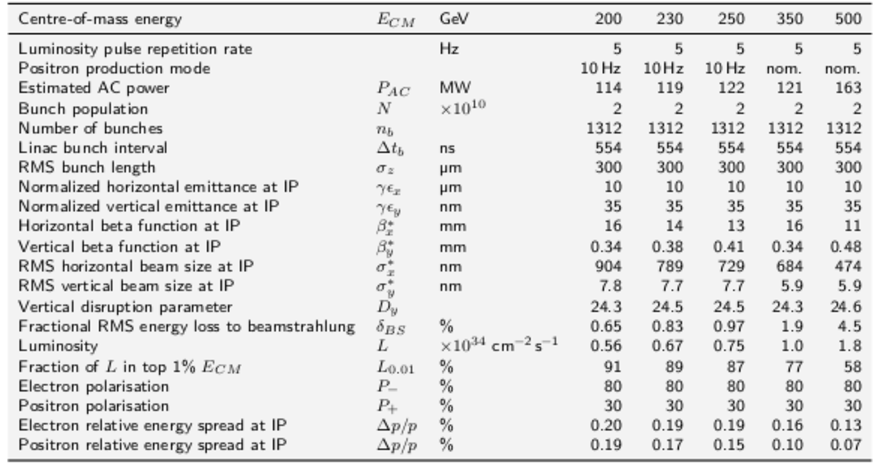
\includegraphics[width=\textwidth]{figures/ILCTDR-VOLUME_3-PART_II_ILCparameters.pdf}
\end{frame}
%\begin{frame}{ILC parameters for the different upgrade stages}
%\ilclogo
%\centering
%	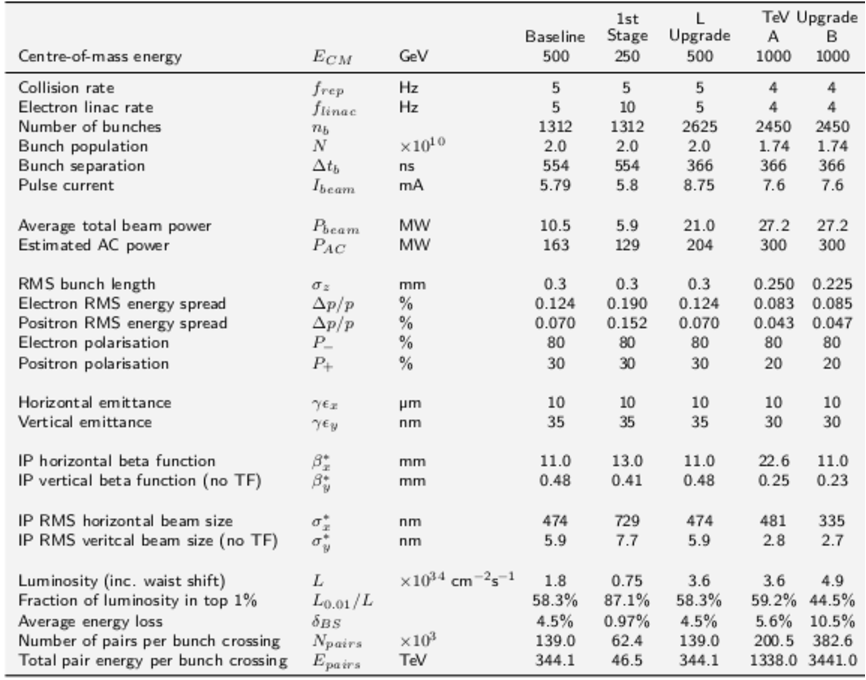
\includegraphics[width=0.8\textwidth]{figures/ILCTDR-VOLUME_3-PART_II_ILCparametersUpgrades.pdf}
%\end{frame}

\section{SiD - Subdetector Specifications}
\begin{frame}
 \begin{table}
\caption{Key parameters of the baseline SiD design, including the measurements of the subdetectors, and their readout cell dimensions. The given readout cell dimension are the pixelation cell sizes used for the full detector Geant4 simulation.}
\label{tab:KeyParametersSiD}
\begin{tabular}{>{\raggedright}p{1.8cm}>{\raggedright}p{2.4cm}>{\raggedright}p{2.2cm}>{\centering}p{1.2cm}>{\raggedright}p{1.2cm}>{\raggedright}p{1.2cm}>{\raggedright}p{1.2cm}}
\hline\hline
\textbf{SiD Barrel} & \textbf{Technology} & \textbf{Readout cell dimensions [mm$^2$]} & \textbf{Inner radius [cm]} & \textbf{Outer radius [cm]} & \textbf{z extent [cm]} \tabularnewline
\hline
Vertex detector & Silicon pixels & 0.05 x 0.05 & 1.4 & 6.0 & $\pm 6.25$ \tabularnewline
Tracker & Silicon strips & 0.05 x 0.05 & 21.7 & 122.1 & $\pm 152.2$ \tabularnewline
ECAL & Silicon pixels- W & 3.5 x 3.5 & 126.5 & 140.9 & $\pm 176.5$ \tabularnewline
HCAL & RPC - steel & 10 x 10 & 141.7 & 249.3 & $\pm 301.8$ \tabularnewline
Solenoid & 5 T SC & - & 259.1 & 339.2 & $\pm 298.3$ \tabularnewline
Flux return & Scintillator- steel & 30 x 30 & 340.2 & 604.2 & $\pm 303.3$ \tabularnewline
\hline
\end{tabular}
\end{table}
\end{frame}

\begin{frame}
 \begin{table}
\begin{tabular}{>{\raggedright}p{1.8cm}>{\raggedright}p{2.4cm}>{\raggedright}p{2.2cm}>{\centering}p{1.2cm}>{\raggedright}p{1.2cm}>{\raggedright}p{1.2cm}>{\raggedright}p{1.2cm}}
\hline\hline
\textbf{SiD Endcap} & \textbf{Technology} & \textbf{Readout cell dimensions [mm$^2$]} & \textbf{Inner z [cm]} & \textbf{Outer z [cm]} & \textbf{Outer radius [cm]} \tabularnewline
\hline
Vertex detector & Silicon pixels & 0.05 x 0.05 & 7.3 & 83.4 & 16.6 \tabularnewline
Tracker & Silicon strips & 0.05 x 0.05 & 77.0 & 164.3 & 125.5 \tabularnewline
ECAL & Silicon pixel- W & 3.5 x 3.5 & 165.7 & 180.0 & 125.0 \tabularnewline
HCAL & RPC - steel & 10 x 10 & 180.5 & 302.8 & 140.2 \tabularnewline
Flux return & Scintillator- steel & 30 x 30 & 303.3 & 567.3 & 604.2 \tabularnewline
LumiCal & Silicon- W & 3.5 x 3.5 & 155.7 & 169.55 &  20.0 \tabularnewline
BeamCal & Semicond.- W & 3.5 x 3.5 & 326.5 & 344 & 14.0 \tabularnewline
\hline\hline
\end{tabular}
\end{table}
\end{frame}

\section{Background from High Cross Section ILC Processes}
\subsection{FCAL Occupancy}
\begin{frame}{Occupancy in the FCAL}
  \begin{center}
     \includegraphics[width=0.7\textwidth]{figures/fig_raw_occupancy.png}
  \end{center}
  Number of hits per channel during a full ILC bunch train ($\sim$2600 bunch crossings).\\
  {\hfill \tiny Study done by B. Schumm and students at UCSC}
\end{frame}


\subsection{Pair background timing}
\begin{frame}{Creation time of particles hitting the Vertex Detector}
\begin{columns}
 \begin{column}{0.5\textwidth}
Distribution of the time of creation (relative to the bunch crossing) of pair background particles (from 1312 bunches) that hit the endcaps of the VXD.
At the time of the bunch crossing about \num{1.6e6} particles are created (underflow bin).\\
 {\footnotesize The creation time is plotted for pair background particles hitting the vertex endcaps only. This is to avoid double counting of particles that would hit both, the barrel and the endcaps.}
 \end{column}
 \begin{column}{0.55\textwidth}
 \includegraphics[width=1\textwidth]{figures/creationtime_histo_SiVertexEndcap_SiDNote.pdf}
 \end{column}
\end{columns}
 %\adjustbox{max height=\dimexpr\textheight-5.5cm\relax,
%           max width=\textwidth}{
\begin{table}
\footnotesize
\begin{tabular}{>{\RaggedRight}p{1.8cm}>{\RaggedRight}p{1.9cm}>{\RaggedRight}p{1.7cm}>{\RaggedRight}p{2.4cm}>{\RaggedRight}p{2.3cm}}
Overall pairs & Primary pairs [\unit[0]{ns};\unit[11]{ns}] & Late pairs ]\unit[11]{ns};\unit[50]{ns}] & Out-of-time backscatter pairs ]\unit[50]{ns};\unit[554]{ns}] & Out-of-time backscatter pairs ]\unit[554]{ns};\unit[1000]{ns}]\\
\hline
$\sim$ \num{1.9e6} & 87.33\% & 12.38\% & 0.16\% &  0.029\% 
\end{tabular}
\end{table}
%}
\end{frame}

\begin{frame}{Momentum distribution particles hitting the Vertex Detector}
  \includegraphics[width=0.5\textwidth]{figures/momentum_histo_SiVertexBarrelSiVertexEndcap_SiDNote.pdf}
  \includegraphics[width=0.5\textwidth]{figures/transvmomentum_histo_SiVertexBarrelSiVertexEndcap_SiDNote}\\
  Distributions of the pair background particle momenta of pair background particles from 1312 bunches that will hit the barrel and the endcaps of the vertex detector.
  The plots show the histograms of the total and the transverse momenta of the particles hitting the vertex detector, in certain time intervals.
\end{frame}

\subsection{Pair background helixes}
\begin{frame}{Explanation of helix track calculations}
\proceedigHelix
 \begin{center}
  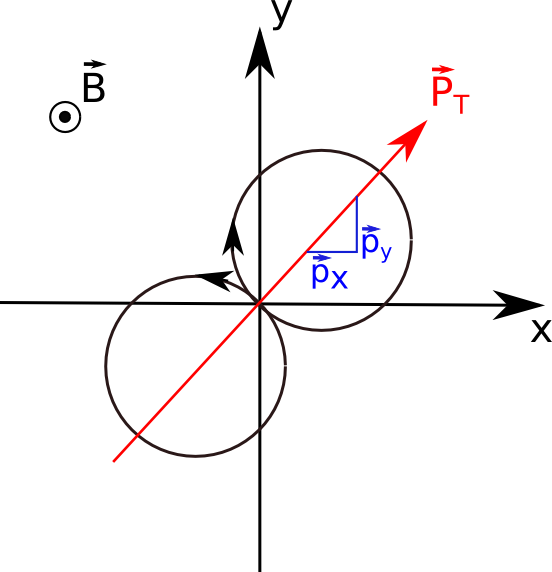
\includegraphics[width=0.65\textwidth]{figures/Helix_explanation.png}
\end{center}
\end{frame}

\section{Muons from the BDS}
\begin{frame}{The Muons in SiD - Spatial Distribution}
\proceedigBDS
 \includegraphics[width=0.9\textwidth]{figures/Explanation_Spatial_distribution_NEW.pdf}
\end{frame}

\begin{frame}{The Muon Occupancy in SiD}
\proceedigBDS
 \includegraphics[width=0.6\textwidth]{figures/Hits_in_SiD_subdetectors_MuonSpoilerStudy.pdf}
  \includegraphics[width=0.45\textwidth]{figures/Explanation_Hits_Subdetectors.pdf}\\
The number of hits in the different SiD subdetectors for both shielding scenarios (\textcolor{Red}{``5 Spoilers''} and \textcolor{Blue}{``5 Spoilers + Wall''}) is not evenly distributed.\\
The number of hits depends on the effective area of the subdetector system.
 \end{frame}
 
 \begin{frame}{Muon Occupancy in SiD HCAL endcaps}
 \proceedigBDS
  \includegraphics[width=0.53\textwidth]{figures/muon_occupancy_deadcells_all_layers_HcalBarrel.pdf}
  \includegraphics[width=0.53\textwidth]{figures/muon_occupancy_deadcells_all_layers_HcalEndcap.pdf}\\
The current SiD electronics design has a \textcolor{Green}{buffer depth of 4}:\\
$\sim$\textcolor{Blue}{1$\times$10\textsuperscript{-6}} - \textcolor{Red}{4$\times$10\textsuperscript{-6}} of all hits are dead in the \textbf{HCAL barrel}\\
$\sim$\textcolor{Blue}{2$\times$10\textsuperscript{-4}} - \textcolor{Red}{1$\times$10\textsuperscript{-3}} of all hits are dead in the \textbf{HCAL endcaps}
\end{frame}

\begin{frame}{Muon Occupancy in SiD Tracker endcaps}
\proceedigBDS
\begin{center}
  \includegraphics[width=0.65\textwidth]{figures/SiTrackerEndcap_DeadCells.png}
\end{center}
The current SiD electronics design has a \textcolor{Green}{buffer depth of 4}, i.e. \textcolor{Blue}{10\textsuperscript{-8}} - \textcolor{Red}{10\textsuperscript{-7}} of all hits are dead in the Tracker endcaps.
\end{frame}
 
\begin{frame}{The Muon Energy}
\proceedigBDS
\begin{center}
  \includegraphics[width=0.65\textwidth]{figures/muon_energy.pdf}
\end{center}
The energy distribution of the muons from the ``5 Spoilers + Wall'' scenario does not reach the same maximum energy. The muons are decelerated and stopped within the magnetized wall.
\end{frame}

\end{document}
\end{appendix}

\cleardoublepage
%\include{Misc/notation}            %%% list of all Your used notation
%\chapter*{Bibliography}
\addcontentsline{toc}{chapter}{Bibliography}
%\bibliography{Misc/bibliography}              %%% include the bibliography 
\printbibliography
%TODO : change the bibtex style 'misc' to 'techreport' for the SiDBkgNote as soon as it is published in a magazine        %%% list of all Your used sources
%%% the acknowledgements
%%% put them on a page on their own, but show them without number in the toc
\chapter*{Acknowledgements}
\addcontentsline{toc}{chapter}{Acknowledgments} 


\backmatter                                    %%% put here whatever You choose

\end{document}


%%%%%%%%%%%%%%%%%%%%%%%%%%%%%%%%%%%%%%%%%%%%%%%%%%%%%%%%%%%%
%%% TODO: Collimator jaw sizes, ATF beam parameters
%%%%%%%%%%%%%%%%%%%%%%%%%%%%%%%%%%%%%%%%%%%%%%%%%%%%%%%%%%%%
